\documentclass[preprint,12pt,sort&compress]{elsarticle}
\usepackage[utf8]{inputenc}
\usepackage{color}
\usepackage{graphicx}
\usepackage{placeins}
\usepackage[margin=1in]{geometry}
\usepackage{appendix}
\usepackage{amsmath, amssymb, bm}
\usepackage{multirow}
\usepackage{placeins}
\usepackage{xfrac}
\usepackage[colorlinks=true, linkcolor=blue, citecolor=blue]{hyperref}
\usepackage[nameinlink, capitalize]{cleveref}
\usepackage[font=footnotesize, labelfont=bf]{caption}
\usepackage{subcaption}
\usepackage[version=4]{mhchem}
\usepackage{lineno}
\usepackage{bm}
\usepackage{comment}
\usepackage[T1]{fontenc}
\usepackage{anyfontsize}
% \usepackage{newtxtext, newtxmath}
\newcommand{\?}{\stackrel{?}{=}}
\usepackage{tablefootnote}
\usepackage{float}
\usepackage{enumitem}
\setlist{itemsep=0pt, topsep=0pt}

% \usepackage{nomencl}
% \makenomenclature
% \setlength{\nomlabelwidth}{2.5cm}  % align descriptions

\journal{Journal of Nuclear Materials}

\begin{document}

\begin{frontmatter}

\title{Modeling oxygen-void interactions in uranium nitride}

\author[ncsu]{Mohamed AbdulHameed}
\author[lanl]{Anton J. Schneider}
\author[ncsu,inl]{Benjamin Beeler\corref{a}}
\ead{bwbeeler@ncsu.edu}
\author[lanl]{Michael W.D. Cooper\corref{b}}
\ead{cooper_m@lanl.gov}
\cortext[a]{Corresponding author}
\cortext[b]{Corresponding author}

\address[ncsu]{Department of Nuclear Engineering, North Carolina State University, Raleigh, NC 27695}
\address[lanl]{Los Alamos National Laboratory, Los Alamos, NM 87545}
\address[inl]{Idaho National Laboratory, Idaho Falls, ID 83415}

\begin{abstract}

Oxygen impurities in uranium nitride (UN) are reported to influence its swelling behavior under irradiation, yet the underlying mechanism remains unknown. In this work, we develop a first-principles model that quantifies the interaction of oxygen with voids and fission gas bubbles in UN, leading to a reduction in surface energy that can promote swelling. The analysis reveals that segregation of substitutional oxygen at surface nitrogen sites is the primary driver of surface energy reduction, $|\Delta \sigma|$, while oxygen in surface hollow sites plays a minor and sometimes counteracting role. $|\Delta \sigma|$ is most pronounced for small cavities ($R_v$ = 1--10 nm) at intermediate temperatures that coincide with the onset of breakaway swelling in UN. Larger voids require higher temperatures for oxygen adsorption to significantly lower their surface energy. The temperature dependence of $|\Delta \sigma|$ exhibits three regimes: negligible reduction at low temperatures due to sluggish oxygen diffusion, a maximum at intermediate temperatures where oxygen incorporation is optimal, and a decline at high temperatures due to enhanced bulk solubility. A parametric analysis reveals that $|\Delta \sigma|$ depends strongly on both oxygen concentration and cavity size, but is largely insensitive to porosity. Our results suggest that oxygen-induced surface energy reduction is essential for reconciling the mechanistic swelling model of UN with experimental observations.

\end{abstract}

\begin{keyword}
Uranium nitride \sep Oxygen segregation \sep Surface energy reduction \sep Void nucleation \sep Fission gas swelling
\end{keyword}

\end{frontmatter}

\newpage

\linenumbers

\section{Introduction}
\label{intro}

Uranium nitride (UN) is considered a highly promising fuel for fast nuclear reactors, space reactors, and potentially commercial light water reactors, due to its high uranium density and high thermal conductivity relative to UO$_2$ \cite{Wallenius2020, Uno2020}. However, early use of UN was limited by issues such as rapid oxidation in air, poor tolerance to water and steam, difficulty in sintering, and the need for nitrogen enrichment with N-15 due to the high neutron absorption of N-14 \cite{Wallenius2020, Uno2020}. Furthermore, many aspects of its behavior at high temperatures and under irradiation remain poorly understood, with scarce experimental data and incomplete mechanistic pictures \cite{Wallenius2020, Uno2020}. Several studies have sought to address this knowledge gap by, for instance, offering an atomistic-level understanding of the deformation mechanisms in UN \cite{AbdulHameed2024b, AbdulHameed2024c}, which play a critical role in pellet–clad mechanical interactions. Additionally, a mechanistic multiscale model has been developed to describe its swelling behavior \cite{Rizk2025}.

UN experiences pronounced swelling driven by the growth of fission gas bubbles to sizes larger than those observed in UO$_2$ \cite{Ronchi1975, Ronchi1978, Rizk2025}, making dimensional stability a key concern for this fuel. The mechanistic model by Rizk \textit{et al.} \cite{Rizk2025} gives a multiscale description of fission-gas swelling and release in UN, coupling atomistic defect data to the BISON finite-element framework via the Simple Integrated Fission Gas Release and Swelling (SIFGRS) model. Their calculations, however, employed a constant void/bubble surface energy derived for oxygen-free UN.

A major challenge in utilizing UN as a nuclear fuel is the presence of oxygen impurities, which can markedly affect its swelling characteristics. Rogozkin \textit{et al.} \cite{Rogozkin2003} demonstrated that fuel swelling becomes substantially more pronounced when the oxygen concentration in UN surpasses the range of 1000 to 1500 parts per million (ppm). Consequently, Schuler \textit{et al.} \cite{Schuler2017} recommended limiting the maximum permissible oxygen content to 1000--1500 ppm to maintain dependable performance of fuel elements. Nevertheless, achieving UN powders with oxygen levels below 1500 ppm has thus far only been accomplished under controlled laboratory conditions \cite{Schuler2017}. This highlights the importance of investigating how oxygen interacts with UN's microstructural features, like voids and bubbles. 

Additionally, mechanistic models that aim to predict fission gas swelling in UN require knowledge of surface energies. Surface energy is a core input to the SIFGRS model utilized by Rizk \textit{et al.} \cite{Rizk2025} as it sets both the equilibrium pressure inside a bubble as a function of its radius, and the contact angle of intergranular bubbles. Therefore, understanding whether oxygen significantly alters the surface energy of voids or gas bubbles is essential for accurately modeling swelling behavior.

The effect of light impurities, such as oxygen, on vacancy cluster morphology has been extensively studied in metals like copper, nickel, and stainless steel \cite{Zinkle1987a, Zinkle1987b, Zinkle1990, Igata1998}. These studies have utilized elastic continuum models \cite{Zinkle1987a, Zinkle1987b}, thermodynamic models \cite{Zinkle1990}, and reaction rate theory \cite{Igata1998} to understand the interaction between impurities and void embryos among other vacancy cluster types. Usually, oxygen impurities impact swelling in metals and alloys by segregating around void surfaces, lowering their surface energy, thereby reducing the critical void radius in the void nucleation stage \cite{Zinkle1987a, Igata1998}. Experimental evidence from metal studies supports the notion that oxygen reduces the surface energy of small voids, typically around 50 vacancies \cite{Zinkle1990}. This reduction in surface energy is a key factor in stabilizing voids and fission-gas bubbles and may similarly affect the swelling behavior in UN. More strikingly, the theoretical studies by Zinkle \textit{et al.} \cite{Zinkle1987a, Zinkle1987b} predict that void formation in high-purity metals is energetically unfavorable, and impurities like oxygen are essential for voids to form. That is, void formation is greatly reduced or even suppressed in low-oxygen metals and alloys. It has been further suggested that oxygen might stabilize void embryos by preventing their collapse into dislocation loops, even if it does not directly reduce surface energy \cite{Zinkle1987b, Zinkle1990}.

Several first-principles studies have explored the properties of oxygen impurities in bulk UN and on its surfaces, calculating the oxygen incorporation, migration, and adsorption energies \cite{Kotomin2008, Kotomin2009, Zhukovskii2009JNM, Zhukovskii2009SS, Bocharov2011JNM, Bocharov2011SS, Bocharov2013, Lopes2016, Schuler2017, Zergoug2018, Sikorski2021}. These studies have demonstrated that oxygen atoms prefer to incorporate into pre-existing nitrogen vacancies, both in bulk UN and on the surface, rather than occupying tetrahedral interstitial sites \cite{Kotomin2008, Bocharov2013}. Oxygen impurities also reduce the migration energy of nearby nitrogen vacancies \cite{Kotomin2009}, indicating that oxygen can influence behaviors that depend on defect dynamics, such as creep. Additionally, it has been observed that O$_2$ molecules parallel to the (001) surface can spontaneously dissociate when centered over a hollow site or a nitrogen atom \cite{Zhukovskii2009JNM}.



A particularly relevant study on the effect of oxygen on swelling in UN is that by Schuler \textit{et al.} \cite{Schuler2017}, who investigated the thermodynamic and transport properties of oxygen in UN using a self-consistent mean-field (SCMF) model. The input energies for their model were derived from density functional theory with the addition of a Hubbard $U$ term (DFT+$U$). Schuler \textit{et al.} found that oxygen is thermodynamically more favorable in the bulk of UN rather than on the (001) surface, leading them to conclude that oxygen segregation on surfaces would be driven by kinetic factors rather than by thermodynamics. However, Kocevski \textit{et al.} \cite{Kocevski2022I} later demonstrated that UN modeled using DFT+$U$ exhibits imaginary phonon frequencies, indicating a dynamically unstable crystal structure. Consequently, the defect energetics used in the SCMF model by Schuler \textit{et al.} might need reconsideration. % as they were based on a dynamically unstable structure.

Oxygen occurs in fresh UN fuel in solution or as a separate UO$_2$ phase, dependent on O concentration and temperature \cite{Lyubimov2014}. UO$_2$ precipitates have been observed experimentally in regions of UN samples where the local oxygen concentration apparently exceeded the solubility limit \cite{Mishchenko2021}. Additionally, DFT studies indicate that oxygen interaction with UN surfaces can lead to the formation of oxynitrides (UO$_x$N$_y$) or pseudo-UO$_2$ structures \cite{Bocharov2013, Lopes2016}.

In this work, we use DFT data to parametrize a thermodynamic model based on defect reactions to study how oxygen impurities interact with voids and fission-gas bubbles in UN. Our model focuses on oxygen adsorption onto void surfaces, where it may reduce surface energy and potentially influence swelling. Throughout this work, we assume that inert gas atoms have no impact on surface energy; therefore, the surface energies of voids and fission-gas bubbles are considered identical. To the best of our knowledge, this is the first study that attempts to quantify the extent to which oxygen interaction with void surfaces affects the void nucleation behavior in UN. We assume that oxygen is the only impurity present, and do not account for the formation of UO$_2$. These simplifications allow us to concentrate on the primary thermodynamic factors that govern the interaction of oxygen with voids, providing an initial step toward understanding the role of oxygen in UN swelling.

\section{Methodology}

\subsection{DFT calculations}

DFT calculations performed in this work utilize the Vienna Ab-initio Simulation Package (VASP) \cite{Kresse1993, Kresse1996a, Kresse1996b} using the Perdew-Burke-Ernzerhof (PBE) \cite{Perdew1996} generalized gradient approximation (GGA) to the exchange-correlation (XC) functional. The pseudopotential models of uranium, nitrogen, and oxygen are based on the projector augmented wave (PAW) method \cite{Kresse1999} where the valence electron configuration of U is $6s^2$ $6p^6$ $6d^2$ $5f^2$ $7s^2$ (14 electrons), that of N is $2s^2$ $2p^3$ (5 electrons), and that of O is $2s^2$ $2p^4$ (6 electrons). Methfessel and Paxton’s smearing method \cite{Methfessel1989} of the first order is used with a width of 0.1 eV to determine the partial occupancies for each wavefunction. $3 \times 3 \times 3$ supercells of ferromagnetic (FM) UN are used to model bulk UN and to study the properties of defects and impurities. To study surface properties, 6-layer and 8-layer symmetric slabs of FM UN are used, where the vacuum gap in each is twice the length of the slab along the $z$-direction. It was shown by Kocevski \textit{et al.} \cite{Kocevski2022I} that the FM ordering provides a suitable model of UN at 0 K. Brillouin zone sampling is performed using Monkhorst-Pack \cite{Monkhorst1976} $3 \times 3 \times 3$ and $3 \times 3 \times 1$ \textit{k}-point meshes for the $3 \times 3 \times 3$ supercells and the symmetric slabs, respectively. In all energy minimization calculations, we set the cutoff energy of the plane-wave basis as 520 eV, the electronic relaxation convergence criterion as $10^{-4}$ eV, and the ionic relaxation convergence criterion as $10^{-2}$ eV/\AA. The nudged elastic band (NEB) method \cite{Henkelman2000a} with the climbing image algorithm \cite{Henkelman2000b} is used to calculate the migration energies of O$_i$ and $\{\text{O}_\text{N} \! : \! v_\text{N}\}$. The structures and ionic minimization trajectories are visualized using OVITO \cite{Stukowski2010} and VESTA \cite{Momma2008}.

% Equations

Point defect formation energies are calculated from:
\begin{equation}
E_f = E_d - E_p - \sum_i n_i \mu_i,
\end{equation}
where $E_d$ and $E_p$ are the energies of the supercell with and without the defect, respectively, $n_i$ is the number of atoms of type $i$ removed ($n_i < 0$) or added ($n_i > 0$) to form the defect, and $\mu_i$ is the chemical potential of the \textit{i}th species.

The U and N chemical potentials are calculated from \cite{AbdulHameed2024}:
\begin{equation}
E_c(\text{U}_{x}\text{N}_{y}) = x \mu_{\ce{U}} + y \mu_{\ce{N}},
\label{Eq:ChemPot}
\end{equation}
where $E_c(\ce{U$_{x}$N$_{y}$})$ is the cohesive energy (energy per formula unit) of compound U$_x$N$_y$. \cref{Eq:ChemPot} is solved for UN and $\alpha$-U to get the U-rich chemical potentials, and for UN and $\alpha$-\ce{U2N3} to get the N-rich chemical potentials \cite{Huang2020, Yang2021}. The chemical potentials at the intermediate near-stoichiometric conditions are the averages of these two bounds \cite{Woodward1998}.

The binding energy of a defect cluster $\{\text{A}_\text{X} \! : \! \text{B}_\text{Y}\}$ is calculated from:
\begin{equation}
E_b = E(\{\text{A}_\text{X} \! : \! \text{B}_\text{Y}\}) + E_p - E(\text{A}_\text{X}) - E(\text{B}_\text{Y}),
\end{equation}
where $E(\cdot)$ is the energy of the supercell containing the relevant defect. Based on this formulation, a negative $E_b$ means binding is favorable.

The incorporation energy of an impurity B in a defect $v_\text{X}$ to form B$_\text{X}$ is calculated from:
\begin{equation}
E_\text{inc} = E( \text{B}_\text{X} ) - E( v_\text{X} ) - \mu_\text{B},
\end{equation}
where $\mu_\text{B}$ is the chemical potential of the impurity in its reference state. The oxygen chemical potential is discussed in \cref{Sec:uO}. Note that $E( v_i ) = E_p$, where $v_i$ denotes a vacant interstitial site. % The solution energy of the same impurity is $E_s = E_i + E_f$ where $E_f$ is the formation energy of $v_\text{X}$. Note also that for an impurity in $v_i$, $E_\text{sol} = E_\text{inc}$ because $v_i$ has no formation energy.

The surface energy is calculated from \cite{Finnis2005}:
\begin{equation}
\sigma = \frac{1}{A} \left( E^* - \sum_{i} N_i \mu_i \right),
\label{Eq:Sigma}
\end{equation}
where $E^*$ is the total DFT energy of the supercell containing the surface, $A$ is the total surface area, $N_i$ is the number of atoms of species $i$ in the supercell containing the surface, and $\mu_i$ is the corresponding chemical potential. Note that $i$ $\in$ \{U, N, O\}.

The adsorption energy is calculated from:
\begin{equation}
E_\text{ad} = \frac{1}{N_\text{ad}} \left( E_\text{surf+ad} - E_\text{surf} \right) - \mu_\text{ad},
\label{Eq:Ead}
\end{equation}
where $E_\text{surf+ad}$ and $E_\text{surf}$ are the energies of the symmetric slabs with and without the adsorbed atom(s), $N_\text{ad}$ is the number of adsorbed atoms, and $\mu_\text{ad}$ is their chemical potential. 

Finally, it is of interest to estimate the change in the surface energy upon oxygen adsorption or surface defect formation. This is accomplished by using the following expression, which is derived in \ref{App2}:
\begin{equation}
\Delta \sigma = \frac{8}{3} \frac{1-p}{p} \frac{R_v}{a^3} c_\text{O} \left[ \alpha_1 \frac{ [ \text{O}_\text{N}^{\text{(s)}} ] }{ [ \text{O}_\text{N}^{\text{(b)}} ] }  E_\text{ad}( \text{O}_\text{N}^{\text{(s)}} ) + \alpha_2 \frac{ [ \text{O}_i^{\text{(s)}} ] }{ [ \text{O}_\text{N}^{\text{(b)}} ] }  E_\text{ad}( \text{O}_i^{\text{(s)}} ) \right] + \frac{2}{a^2} [ v_\text{N}^{\text{(s)}} ] E_f ( v_\text{N}^{\text{(s)}} ),
\label{Eq:DeltaSigma1}
\end{equation}
where $p$ is the porosity, $R_v$ is the average void radius, $a$ is the lattice constant, $c_\text{O}$ is the atomic oxygen concentration, and $\alpha_1$ and $\alpha_2$ are the kinetic corrections for the defects $\text{O}_\text{N}^\text{(s)}$ and $\text{O}_i^{\text{(s)}}$, respectively. For a defect $i$, $\alpha_i$ is defined as \cite{Zinkle1990}:
\begin{equation}
\alpha_i =
\begin{cases}
    \sqrt{D_i t}/\lambda_v & \text{if } \sqrt{D_i t}/\lambda_v < 1, \\
    1 & \text{if } \sqrt{D_i t}/\lambda_v \geq 1,
\end{cases}
\label{Eq:alpha}
\end{equation}
where $D_i$ is the diffusivity of the relevant defect, $t$ is the void nucleation time, and $\lambda_v$ is the mean free path between voids, defined as $\lambda_v = n_v^{-1/3}$, where $n_v = p / ( \frac{4}{3} \pi R_v^3 )$ is the void number density. We assume a void nucleation time $t$ = 42 hours. This estimate is justified by taking a typical dose rate, $\dot{G}$, in a fast reactor core as on the order of $10^{-6}$~dpa/s~\cite{Mansur1983, Saha2018}. In stainless steels, stable voids are fully formed by a dose, $G$, in the range of 0.1--0.2~dpa~\cite{Surh2004}. Using the relation $t = G / \dot{G}$, this corresponds to a void nucleation time between 28 and 56 hours, with an average of 42 hours. Due to the lack of experimental data on early-stage void nucleation in UN fuels, this estimated time serves as a reasonable placeholder, but with unknown uncertainty. Note that \cref{Eq:DeltaSigma1} predicts that the surface energy reduction scales linearly with oxygen concentration.

\subsection{Oxygen chemical potential}
\label{Sec:uO}

DFT calculations with GGA exchange-correlation functionals are known for being inaccurate for gases like \ce{O2} \cite{Bocharov2013}. This is usually remedied by using hybrid functionals or applying semi-empirical corrections \cite{Sargeant2021}. Alternatively, Finnis \textit{et al.} \cite{Finnis2005} suggested using common oxides as the oxygen reference state. For an oxide M$_a$O$_b$, the formation reaction is:
\begin{equation}
a \text{M(s)} + \frac{b}{2} \text{O$_2$(g)} \rightleftharpoons \text{M$_a$O$_b$(s)}.
\end{equation}
The Gibbs free energy balance for this reaction is:
\begin{equation}
\Delta_f G^0 (\text{M$_a$O$_b$}) = g^0(\text{M$_a$O$_b$}) - a \mu_\text{M}^0 - b \mu_\text{O}^0,
\label{Eq:OChemPot}
\end{equation}
where $\Delta_f G^0 (\text{M$_a$O$_b$})$ is the standard Gibbs free energy of formation for the oxide, which is available in thermochemical tables \cite{Linstrom2024}, $g^0$(M$_a$O$_b$) is approximated by the DFT energy per formula unit of the oxide, $\mu_\text{M}^0$ is approximated by the DFT energy per atom of the metal, and $\mu_\text{O}^0$ is the oxygen chemical potential. The superscript 0 on any quantity denotes its value at the standard pressure, $P^0$ = 1 bar, and standard temperature, $T^0$ = 298.15 K. Approximating $T^0$ with 0 K in the context of DFT calculations introduces little error \cite{Finnis2005}. Rearranging \cref{Eq:OChemPot}, the oxygen chemical potential is:
\begin{equation}
\mu_\text{O}^0 = \frac{1}{b} \left[ g^0(\text{M$_a$O$_b$}) - a \mu_\text{M}^0 - \Delta_f G^0 (\text{M$_a$O$_b$}) \right].
\label{Eq:OxidePot}
\end{equation}

Finnis \textit{et al.} state that the chemical potential of oxygen should be independent of the specific oxide used. Using \ce{MgO} and \ce{Al2O3} as the initial oxide, we found that the chemical potential for both is $\mu_\text{O} = - 4.18$ eV. This value is used as the reference chemical potential to report all the oxygen incorporation and adsorption energies in \cref{Sec:Results}. However, we are concerned with studying how oxygen interacts with voids in UN, where oxygen atoms are introduced as impurities during manufacturing. For this setting, the oxygen reference state is not the oxide, but rather the most dominant oxygen impurity type, which is $\text{O}_\text{N}^\text{(b)}$ as will be shown in \cref{Sec:Results}. Note that we use the Kröger-Vink notation \cite{Kroger1956} to describe point defects, but with charges omitted because UN exhibits metallic properties and defects have no associated charge \cite{Cooper2023}. Superscripts (b) and (s) are added to the Kröger-Vink notation to differentiate bulk and surface defects, respectively.

The reference state of oxygen impurities in UN is based on the following defect reaction:
\begin{equation}
v_\text{N}^\text{(b)} + \frac{1}{2} \text{O}_2 \text{(g)} \rightleftharpoons \text{O}_\text{N}^\text{(b)},
\end{equation}
which has the following mass-action law:
\begin{equation}
K_1 = \frac{ [ \text{O}_\text{N}^\text{(b)} ] }{ [ v_\text{N}^\text{(b)} ] P_{\text{O}_2}^{1/2} } = \text{exp}\! \left[ - \frac{E( \text{O}_\text{N} ) - E( v_\text{N} )}{kT} \right],
\label{Eq:Kmu}
\end{equation}
where $E( \text{O}_\text{N} )$ and $E( v_\text{N} )$ are the DFT energies of the supercells containing $\text{O}_\text{N}$ and $v_\text{N}$, respectively. This difference is termed the ``raw incorporation energy'' \cite{AbdulHameed2024}, i.e., the incorporation energy without considering the impurity's reference state. The dependence of the oxygen chemical potential on oxygen partial pressure, $P_{\text{O}_2}$, and temperature, $T$, is given by \cite{Finnis2005}:
\begin{equation}
\mu_\text{O}(P_{\text{O}_2}, T) = g(T) + \frac{1}{2} kT \, \text{ln} \!\left( P_{\text{O}_2} / P^0 \right),
\label{Eq:muTPO2}
\end{equation}
where the temperature dependence, $g(T)$, is extracted from thermochemical tables \cite{Linstrom2024}. Focusing on the dependence on the oxygen partial pressure:
\begin{equation}
\mu_\text{O}(P_{\text{O}_2}) = \frac{1}{2} kT \, \text{ln} \!\left( P_{\text{O}_2} / P^0 \right),
\label{Eq:muPO2}
\end{equation}
and rearranging \cref{Eq:muPO2,Eq:Kmu}, it can be easily shown that the oxygen chemical potential is:
\begin{equation}
\mu_\text{O} = E( \text{O}_\text{N} ) - E( v_\text{N} ) + kT \, \text{ln} \! \left( [ \text{O}_\text{N}^\text{(b)} ] / [ v_\text{N}^\text{(b)} ] \right).
\label{Eq:OxygenTruePot}
\end{equation}

\subsection{Oxygen diffusivity}

The diffusivity of oxygen impurities is also explored in this work. The diffusivity of a defect $d$ is calculated from:
\begin{equation}
D_d = \frac{1}{6} z \lambda^2 \nu \, \text{exp}\! \left( - \frac{E_m}{ k T } \right),
\label{Eq:Diffusion}
\end{equation}
\noindent where $d$ $\in$ \{O$_i$, $\{\text{O}_\text{N} \! : \! v_\text{N}\}$\}, $z$ is the number of equivalent sites the atom can jump to, and $\lambda$ is the jump distance. Both $z$ and $\lambda$ are determined from the crystal structure. For O$_i$, $z$ = 6 and $\lambda$ = $a/2$, with $a$ being the lattice constant. For $\{\text{O}_\text{N} \! : \! v_\text{N}\}$, $z$ = 12 and $\lambda$ = $a/\sqrt{2}$. $E_m$ is the effective migration energy. For O$_i$, $E_m$ = 2.41 eV. For $\{\text{O}_\text{N} \! : \! v_\text{N}\}$, net bulk diffusion requires two steps \cite{Kocevski2022II}: (\textit{a}) O$_\text{N}$ and $v_\text{N}$ exchange, and (\textit{b}) $v_\text{N}$ rotation around O$_\text{N}$. Note the $\text{O}_\text{N}$ is immobile by itself and can only move via this two-step process with the assistance of a nearby $v_\text{N}$. The saddle point energy of the exchange step is 2.87 eV, whereas that of the rotation step is 3.06 eV. Based on the highest barrier approximation \cite{Claisse2016}, the effective migration energy is 3.06 eV. % All migration energies calculated in this work are shown in \cref{Tab:Mig}. 

In \cref{Eq:Diffusion}, $\nu$ is the attempt frequency, which can be estimated from phonon calculations. Because these calculations are computationally expensive, we use a semi-classical approach to estimate $\nu$ as \cite{Olander2017}:
\begin{equation}
\nu = \left( \frac{E_m}{2m\lambda^2} \right)^{1/2},
\label{Eq:nu}
\end{equation}
where $m$ is the mass of the diffusing atom. For $\{\text{O}_\text{N} \! : \! v_\text{N}\}$, the limiting step is the rotation of $v_\text{N}$  around O$_\text{N}$ and the mass of the nitrogen atom is used. For O$_i$, the mass of the oxygen atom is used. For the diffusion of $\{\text{O}_\text{N} \! : \! v_\text{N}\}$, $\nu = 9.45~\times~10^{12}$ Hz, whereas for $\text{O}_i$, $\nu = 1.11~\times~10^{13}$ Hz.

% \Cref{Eq:nu} is based on two simplifications: First, at the equilibrium position, the energy of the diffusing impurity is closely represented by the harmonic approximation \cite{Olander2017}:
% \begin{equation}
% U(r) = U(r_0) + \frac{1}{2}  \left( \frac{d^2U}{dr^2} \right)_{r_0} (r - r_0)^2.
% \end{equation}

% \noindent Then, $\nu$ has the form:
% \begin{equation}
% \nu = \frac{1}{2 \pi} \left[ \frac{1}{m} \left( \frac{d^2U}{dr^2} \right)_{r_0} \right]^{1/2}.
% \end{equation}

% \noindent Second, between two equilibrium positions, the energy barrier that the impurity encounters has the following form:
% \begin{equation}
% U(r) = U(r_0) + E_m \, \text{sin}^2 \! \left[ \frac{ \pi (r - r_0) }{ \lambda } \right].
% \end{equation}


The diffusivity of an impurity X by a mechanism that depends on defect $d$ is calculated from \cite{Cooper2023}:
\begin{equation}
D_{X, d} = f \frac{c_d}{c_\text{X}} D_d,
\end{equation}
where $f$ is the correlation factor. For $\{\text{O}_\text{N} \! : \! v_\text{N}\}$, $f$ = 0.7815 \cite{Laughlin2014}, which is the value for vacancy-mediated migration in the FCC nitrogen sublattice. For O$_i$, $f$ = 1 \cite{Laughlin2014}. $c_d$ is the atomic concentration of the defect $d$ and $c_\text{X}$ is the total atomic concentration of impurity X. As an approximation, we assume that $c_\text{O} = [\text{O}_\text{N}]$ which will be justified in \cref{Sec:Oxygen} of the results.

\subsection{Defect reactions}

In this section, we outline the defect reactions used to estimate the relative concentrations of various oxygen defect types. In general, there are three categories of defect reactions: (\textit{a}) reactions that relate defects in the bulk, (\textit{b}) reactions that relate defects on the void surfaces, and (\textit{c}) reactions that thermodynamically dictate defect transitions from the bulk to the void surfaces, and vice versa. A limitation of the latter category of reactions is that it neglects the kinetic aspects of the defect transitions. That is, the kinetics of reactions in (\textit{c}) category are assumed to be faster than those in the (\textit{a}) and (\textit{b}) categories. % and only gives concentrations in the limit of infinite time.

The first bulk defect reaction is:
\begin{equation}
\text{O}_\text{N}^\text{(b)} \rightleftharpoons v_\text{N}^\text{(b)} + \text{O}_i^\text{(b)},
\end{equation}
and its mass-action law is:
\begin{equation}
K_2 = \frac{ [ \text{O}_i^\text{(b)} ]  [ v_\text{N}^\text{(b)} ] } { [ \text{O}_\text{N}^\text{(b)} ] } = \text{exp}\! \left[ - \frac{ E_\text{inc}( \text{O}_i^\text{(b)} ) - E_\text{inc}( \text{O}_\text{N}^\text{(b)} ) } { k T } \right].
\end{equation}

The second bulk defect reaction is:
\begin{equation}
v_\text{N}^\text{(b)} + \text{O}_\text{N}^\text{(b)} \rightleftharpoons \{\text{O}_\text{N} \! : \! v_\text{N}\}^\text{(b)},
\end{equation}
and its mass-action law is:
\begin{equation}
K_3 = \frac{ [ \{\text{O}_\text{N} \! : \! v_\text{N}\}^\text{(b)} ] } { [ v_\text{N}^\text{(b)} ] [ \text{O}_\text{N}^\text{(b)} ] } = \text{exp}\! \left[ - \frac{ E_b( \{\text{O}_\text{N} \! : \! v_\text{N}\}^\text{(b)} ) } { k T } \right].
\end{equation}

The defect reaction at void surfaces is:
\begin{equation}
v_i^\text{(s)} + \text{O}_\text{N}^\text{(s)}  \rightleftharpoons  v_\text{N}^\text{(s)} + \text{O}_i^\text{(s)},
\end{equation}
and its mass-action law is:
\begin{equation}
K_4 = \frac{ [ v_\text{N}^\text{(s)} ]  [ \text{O}_i^\text{(s)} ] } { [ v_i^\text{(s)} ] [ \text{O}_\text{N}^\text{(s)} ] } = \text{exp}\! \left[ - \frac{ E_\text{ad}( \text{O}_i^\text{(s)} ) - E_\text{ad}( \text{O}_\text{N}^\text{(s)} ) } { k T } \right].
\end{equation}

The first reaction that relates bulk UN and the void surface is:
\begin{equation}
v_\text{N}^\text{(b)} + \text{N}_\text{N}^\text{(s)}  \rightleftharpoons v_\text{N}^\text{(s)} + \text{N}_\text{N}^\text{(b)},
\end{equation}
and its mass-action law is:
\begin{equation}
K_5 = \frac{ [ v_\text{N}^\text{(s)} ]  [ \text{N}_\text{N}^\text{(b)} ] } { [ v_\text{N}^\text{(b)} ] [ 
\text{N}_\text{N}^\text{(s)} ] } = \text{exp}\! \left[ - \frac{ E_f ( v_\text{N}^\text{(s)} ) - E_f ( v_\text{N}^\text{(b)} ) } { k T } \right].
\label{Eq:VN-VNs}
\end{equation}
$[ \text{N}_\text{N}^\text{(s)} ]$, the atomic concentration of the nitrogen sites on the surface, can be estimated from knowledge of the porosity, $p$, and the average void radius, $R_v$ by the following expression which is derived in \ref{App1}:
\begin{equation}
[ \text{N}_\text{N}^\text{(s)} ] = \frac{3}{2} \frac{p}{1-p} \frac{a}{R_v},
\label{Eq:NNs1}
\end{equation}
where $a$ is the lattice constant. Note that $[ \text{N}_\text{N}^\text{(b)} ] = 1 - [ \text{N}_\text{N}^\text{(s)} ]$. 

The second reaction is:
\begin{equation}
v_\text{N}^\text{(b)} + \text{O}_i^\text{(s)}  \rightleftharpoons v_i^\text{(s)} + \text{O}_\text{N}^\text{(b)},
\end{equation}
and its mass-action law is:
\begin{equation}
K_6 = \frac{ [ v_i^\text{(s)} ]  [ \text{O}_\text{N}^\text{(b)} ] } { [ v_\text{N}^\text{(b)} ] [ \text{O}_i^\text{(s)} ] } = \text{exp}\! \left[ - \frac{ E_\text{inc}( \text{O}_\text{N}^\text{(b)} ) - E_\text{ad}( \text{O}_i^\text{(s)} ) } { k T } \right].
\end{equation}
As derived in \ref{App1}, $[ v_i^\text{(s)} ]$ is given by:
\begin{equation}
[ v_i^\text{(s)} ] = \frac{3p}{1-p} \frac{a}{R_v}.
\label{Eq:v_i^s}
\end{equation}

To find the relative concentration $[ \text{O}_\text{N}^\text{(s)} ] / [ \text{O}_\text{N}^\text{(b)} ]$, it is not necessary to resort to a defect reaction. Instead, the ratio is calculated from: 
\begin{equation}
\frac{ [ \text{O}_\text{N}^\text{(s)} ] }{ [ \text{O}_\text{N}^\text{(b)} ] } = \frac{ [ \text{O}_i^\text{(s)} ] }{ [ \text{O}_\text{N}^\text{(b)} ] } \div \frac{ [ \text{O}_i^\text{(s)} ] }{ [ \text{O}_\text{N}^\text{(s)} ] } = \frac{ [v_\text{N}^\text{(s)}] }{ [v_\text{N}^\text{(b)}] } \, \text{exp}\! \left[ - \frac{ E_\text{ad}( \text{O}_\text{N}^\text{(s)} ) - E_\text{inc}( \text{O}_\text{N}^\text{(b)} ) } { k T } \right].
\label{Eq:ONs_ONb}
\end{equation}

\section{Results}
\label{Sec:Results}

\subsection{Defect energetics}
\label{Sec:DefE}

The formation energies of U and N vacancies in UN are shown in \cref{Tab:EfVN}. The bulk formation energies compare very well with those calculated by Yang and Kaltsoyannis \cite{Yang2021} and Kocevski \textit{et al.} \cite{Kocevski2022I}. It is noticed that there is a consistent difference of about 0.76 eV between N vacancy formation on the surface and in the bulk, independent of stoichiometry. This difference is termed the segregation energy of the N vacancy. It is easier to form an N vacancy on the surface than in the bulk, and the number of $v_\text{N}^\text{(s)}$ sites is limited by the available surface area.

\begin{table}[h!]
\scriptsize
\centering
\caption{Formation energies (eV) of U and N vacancies in UN. Reference energies are DFT values calculated by Yang and Kaltsoyannis \cite{Yang2021} and Kocevski \textit{et al.} \cite{Kocevski2022I}.}
\begin{tabular}{l|cc|cc|cc}
\hline
 & \multicolumn{2}{c|}{U-rich} & \multicolumn{2}{c|}{Intermediate} & \multicolumn{2}{c}{N-rich} \\
& Calc. & Ref. & Calc. & Ref. & Calc. & Ref. \\
\hline
$v_\text{U}^\text{(b)}$ & 3.28 & 3.17--3.43 \cite{Yang2021}, 3.27--3.86 \cite{Kocevski2022I} & 2.79 & 2.75--3.01 \cite{Yang2021} & 2.30 & 2.34--2.60 \cite{Yang2021}, 2.09--2.58 \cite{Kocevski2022I} \\
$v_\text{N}^\text{(b)}$ & 1.64 & 1.76--1.90 \cite{Yang2021}, 0.62--1.86 \cite{Kocevski2022I} & 2.13 & 2.18--2.31 \cite{Yang2021} & 2.62 & 2.59--2.72 \cite{Yang2021}, 1.42-2.82 \cite{Kocevski2022I} \\
$v_\text{N}^\text{(s)}$ & 0.88 & --   & 1.37 & -- & 1.86 & --   \\
\hline
\end{tabular}
\label{Tab:EfVN}
\end{table}

The incorporation energies of oxygen in UN are shown in \cref{Tab:Einc}, all given relative to $\mu_\text{O} = - 4.18$ eV. The most favorable oxygen defect in the bulk is $\text{O}_\text{N}$ followed by $\text{O}_i$. We also attempted to calculate the incorporation energy of the $\langle 111 \rangle$ and $\langle 110 \rangle$ O-N dumbbells. The $\langle 111 \rangle$ O-N dumbbell has a larger incorporation energy ($-1.11$ eV) than the tetrahedral site, whereas the $\langle 110 \rangle$ O-N dumbbell is unstable and relaxes to the $\langle 111 \rangle$ configuration. The largest incorporation energy is that of $\text{O}_\text{U}$, which indicates that O impurities exist almost exclusively in the N-sublattice.
% as confirmed by visual inspection of the ionic minimization trajectory using OVITO.

\begin{table}[h!]
\centering
\caption{Incorporation energies of oxygen in UN for $\mu_\text{O} = - 4.18$ eV. This value of $\mu_\text{O}$ is calculated according to the Finnis \textit{et al.} \cite{Finnis2005} oxide method.}
\footnotesize
\begin{tabular}{lc}
\hline
Defect & Incorporation energy [eV] \\
\hline
O$_\text{N}$ & $-7.23$ \\
O$_i$          & $-2.94$ \\
$\langle 111 \rangle$ O-N dumbbell & $-1.11$ \\
$\langle 110 \rangle$ O-N dumbbell & Unstable \\
O$_\text{U}$ & $-0.40$ \\
\hline
\end{tabular}
\label{Tab:Einc}
\end{table}

The binding energies of the explored defect clusters are shown in \cref{Tab:Eb}, where negative values indicate favorable binding. The most relevant defect cluster to our study, i.e., $\{\text{O}_\text{N} \! : \! v_\text{N}\}$, has a binding energy of 0.03 eV, which is practically zero. That is, binding is neither favorable nor unfavorable, and the N vacancy can roam around independently of $\text{O}_\text{N}$. On the other hand, we found a strong tendency for binding between $\text{O}_\text{N}$ and $v_\text{U}$, $\text{Kr}_\text{U}$, and $\text{Xe}_\text{U}$, all with an average binding energy of about $-0.4$ eV. We propose that this binding may promote the initial aggregation of defects into void or bubble embryos. This finding is consistent with experimental observations by Turos \textit{et al.} \cite{Turos1990}, who reported that Kr and Xe atoms form impurity-defect complexes in UN, serving as precursors for gas bubble formation. A comparable phenomenon is observed with helium in copper \cite{Zinkle1987b}, where helium does not reduce the void surface energy but stabilizes void embryos by binding with vacancies and vacancy clusters. A similar role may be played by oxygen in UN, potentially contributing to the stabilization of voids and bubbles. Due to the low concentrations of $\text{Kr}_\text{U}$ and $\text{Xe}_\text{U}$, we anticipate that this effect is less significant than the direct reduction of surface energy through oxygen adsorption.

\begin{table}[h!]
\centering
\caption{Binding energies of defect clusters in UN. Negative values mean that binding is favorable and vice versa.}
\footnotesize
\begin{tabular}{lc}
\hline
Defect cluster & Binding energy [eV] \\
\hline
$\{\text{O}_\text{N} \! : \! v_\text{N}\}$  & $0.03$  \\
$\{\text{O}_\text{N} \! : \! v_\text{U}\}$  & $-0.40$ \\
$\{\text{O}_\text{N} \! : \! \text{Kr}_\text{U}\}$ & $-0.41$ \\
$\{\text{O}_\text{N} \! : \! \text{Xe}_\text{U}\}$ & $-0.39$ \\
\hline
\end{tabular}
\label{Tab:Eb}
\end{table}

The migration energies of defects relevant to this study are shown in \cref{Tab:Mig}. As can be expected, the migration energy of $\text{O}_i$ is smaller than that of $\{ \text{O}_\text{N} \! : \! v_\text{N} \}$, which is 3.06 eV based on the highest barrier approximation. It is predicted that the migration energy of $v_\text{N}$ is slightly reduced from 3.10 to 3.06 eV when an $\text{O}_\text{N}$ is in a first nearest neighbor position. A similar observation has been made by Kotomin \textit{et al.} \cite{Kotomin2009}.

\begin{table}[h!]
\centering
\caption{Migration energies of some defects and/or migration paths in UN.}
\footnotesize
\begin{tabular}{lc}
\hline 
Defect and/or migration path & Migration energy [eV] \\
\hline
$v_\text{N}$ & 3.10 \\
O$_i$          & 2.41 \\
O$_\text{N}$-$v_\text{N}$ exchange & 2.87 \\
$v_\text{N}$ rotation around O$_\text{N}$ & 3.06 \\
\hline
\end{tabular}
\label{Tab:Mig}
\end{table}

\subsection{UN surface properties}

% The N atoms are slightly above the U atoms by 0.09 \AA\ for the first outermost layer (i.e., the layer in contact with the vacuum gap), and by 0.03 \AA\ for the second layer. For the 3rd layer, however, the N atoms are below the U atoms by 0.01 \AA. This emphasizes the importance of investigating a system with a minimum of 6 layers to avoid surface-surface interactions in the supercell. The average distances between different layers are shown in \cref{Tab:d}, with the subscript defining the layer number with respect to the surface. The decrease of $d_{12}$ (relative to $d_{\infty}$) and the accompanying increase of $d_{23}$ can be explained by bond-order conservation \cite{Taylor2008}, i.e., stronger bonding of the second layer with the upper first layer will lead to weakened bonding with the lower third layer.

% \begin{figure}[h!]
%     \centering
%     \includegraphics[width=0.7\textwidth]{Surf8.png}
%     \caption{(Color online) A view along the [110] direction of the first 4 layers of the 8-layer surface showing slight surface reconstruction. Distances in \cref{Tab:d} are also outlined. U atoms are brown, and N atoms are gray.}
%     \label{Fig:Surf8}
% \end{figure}

% \begin{table}[h!]
% \centering
% \caption{Distances between the surface layers for the 8-layer (001) surface in UN. $d_{12}$ refers to the distance between the first and second layers, and so on. $d_\infty$ refers to the distance between the layers in bulk UN. The percent change of the distances relative to $d_\infty$ is shown in parentheses. Distances are also outlined in \cref{Fig:Surf8}.}
% \footnotesize
% \begin{tabular}{lc}
% \hline
% $d_{12}$ & 2.409 \AA\ ($-0.91$\%) \\
% $d_{23}$ & 2.434 \AA\ ($+0.15$\%) \\
% $d_{34}$ & 2.432 \AA\ ($+0.06$\%) \\
% $d_\infty$ & 2.431 \AA \\
% \hline
% \end{tabular}
% \label{Tab:d}
% \end{table}

Upon relaxation, the 8-layer UN (001) surface undergoes a slight adjustment of the interlayer spacing, with the maximum interlayer spacing change remaining below 1\%. The energy of the UN (001) surface under various stoichiometric conditions with and without defects is presented in \cref{Tab:SurfE}. It is evident that the surface energies of the 6-layer and 8-layer slabs are very similar, indicating that the 6-layer slab is sufficient to achieve a converged description of the UN (001) surface. Therefore, the 6-layer slab is used in all subsequent adsorption calculations. Several observations can be made regarding the impact of adsorption on surface energy. Introducing $\text{O}_i^{\text{(s)}}$ onto the pure 6-layer surface decreases its energy by 0.182 J/m$^2$, irrespective of the stoichiometry. Furthermore, the surface energy of the 6-layer surface with $\text{O}_\text{N}^{\text{(s)}}$ is reduced relative to that of the 6-layer surface with $v_\text{N}^{\text{(s)}}$ by 0.256 J/m$^2$, also independent of stoichiometry.

\begin{table}[h!]
\centering
\caption{Surface energies of the UN (001) surface in units of J/m$^2$ as calculated by \cref{Eq:Sigma}.}
\footnotesize
\begin{tabular}{lccc}
\hline
 & U-rich & Intermediate & N-rich \\
\hline
6-layer pure surface & 1.586 & 1.586 & 1.586 \\
8-layer pure surface  & 1.592 & 1.592 & 1.592 \\
6-layer surface with O$_i^\text{(s)}$ & 1.404 & 1.404 & 1.404 \\
6-layer surface with $v_\text{N}^\text{(s)}$ & 1.620 & 1.638 & 1.656 \\
6-layer surface with O$_\text{N}^\text{(s)}$ & 1.364 & 1.382 & 1.400 \\
\hline
\end{tabular}
\label{Tab:SurfE}
\end{table}

The oxygen adsorption sites explored in this work are shown in \cref{Fig:Oad-2} generated using VESTA. Oxygen adsorption energies in different sites on the 6-layer slab are given in \cref{Tab:Ead}. The most stable site is a N surface vacancy, followed by the hollow site, i.e., $\text{O}_i^\text{(s)}$, as was also found in previous studies \cite{Kotomin2008, Bocharov2013}. The adsorption energy of the oxygen in the hollow site does not change if the oxygen atoms are on one or both sides of the slab, which indicates the absence of any polarity effects. Thus, considering only one side of the slab is sufficient for obtaining accurate adsorption energies. Oxygen adsorption energy in a hollow site slightly decreases from $-4.84$ eV to $-4.85$ eV when an oxygen atom is introduced in a nearest neighbor hollow site and increases to $-4.72$ eV for 4 neighboring O atoms forming a square, which is due to the lateral repulsive interaction between closely packed oxygen adsorbate atoms. This suggests that the saturation coverage of oxygen is probably smaller than 1 ($\theta_s < 1$). However, in this model, oxygen-oxygen interactions are neglected, and a saturation coverage of 1 is assumed for all impurity sites. If the actual saturation coverage was, say, $\theta_s = 0.5$, the effect of this would be to divide $[ v_i^\text{(s)} ]$ by 2, which is negligible on a log scale.

Note that the adsorption energy of O atoms in above-U sites is the same as that of O in a hollow site (\cref{Tab:Ead}). To confirm that the above-U site is stable, we shifted the oxygen atom by 0.2 {\AA} toward the hollow site, and it relaxed back to the above-U site. One way to account for the above-U sites in our model is to multiply $[ v_i^\text{(s)} ]$ by 2, as outlined in \ref{App1}. The bridge site is marked as unstable since oxygen atoms in this configuration relax to the above-U position. The largest adsorption energy is that of the above-N site (equivalent to a site on the U sublattice). % which is expected as oxygen does not prefer to exist on the U sublattice, either in bulk (\cref{Tab:Einc}) or on the surface. % This effect is nearly canceled out by the fact that, based only on hollow-site considerations, $\theta_s \sim 0.5$. Thus, \cref{Eq:Vis} is used to account for $[ v_i^\text{(s)} ]$ with no modifications.

\begin{figure}[h!]
    \centering
    \includegraphics[width=0.45\textwidth]{Oad-3.png}
    \caption{(Color online) A view of the UN surface along the $z$-axis (i.e., surface normal) showing the different oxygen adsorption sites. U atoms are gray, N atoms are green, and O atoms are red.}
    \label{Fig:Oad-2}
\end{figure}

\begin{table}[h!]
\centering
\caption{Adsorption energy of oxygen into sites on the symmetric 6-layer slab model of the UN (001) surface. These values correspond to $\mu_\text{O} = - 4.18$ eV, which is calculated according to the Finnis \textit{et al.} \cite{Finnis2005} oxide method.}
\footnotesize
\begin{tabular}{lc}
\hline
Adsorption site & Adsorption energy [eV] \\
\hline
$v_\text{N}^\text{(s)}$                      & $-6.80$ \\
Hollow site (one side), i.e., O$_i^\text{(s)}$ & $-4.84$ \\
Hollow site (both sides)                         & $-4.84$ \\
2 nearest-neighbor hollow sites (dumbbell)       & $-4.85$ \\
4 nearest-neighbor hollow sites (square)         & $-4.72$ \\
Bridge site                                      & Unstable \\ % Relaxes to the above-U site 
Above-U site                                     & $-4.83$ \\
Above-N site                                     & $-2.77$ \\
\hline
\end{tabular}
\label{Tab:Ead}
\end{table}

The oxygen adsorption energies in \cref{Tab:Ead} are reported with the chemical potential of oxygen taken from the oxide as the reference state (i.e., \cref{Eq:OxidePot}). As explained earlier, however, the more appropriate oxygen reference state is oxygen pre-existing in UN as an impurity. In this case, the relevant chemical potential is that shown in \cref{Fig:uO}. The adsorption energies of oxygen relative to that chemical potential are shown in \cref{Fig:EadONs,Fig:EadOis} for $\text{O}_\text{N}^\text{(s)}$ and $\text{O}_i^\text{(s)}$, respectively. Comparing these adsorption energies to those in \cref{Tab:Ead}, we can differentiate between two cases: While oxygen adsorption on external surfaces reduces surface energy both as $\text{O}_\text{N}^\text{(s)}$ and $\text{O}_i^\text{(s)}$, pre-existing oxygen in UN adsorbing on internal void surfaces reduces the surface energy only when adsorbing as $\text{O}_\text{N}^\text{(s)}$. In contrast, $\text{O}_i^\text{(s)}$ increases the surface energy of internal void surfaces. This behavior is due to the different reference states of oxygen in both cases. 

\begin{figure}[h!]
\centering
\begin{subfigure}{0.48\textwidth}
    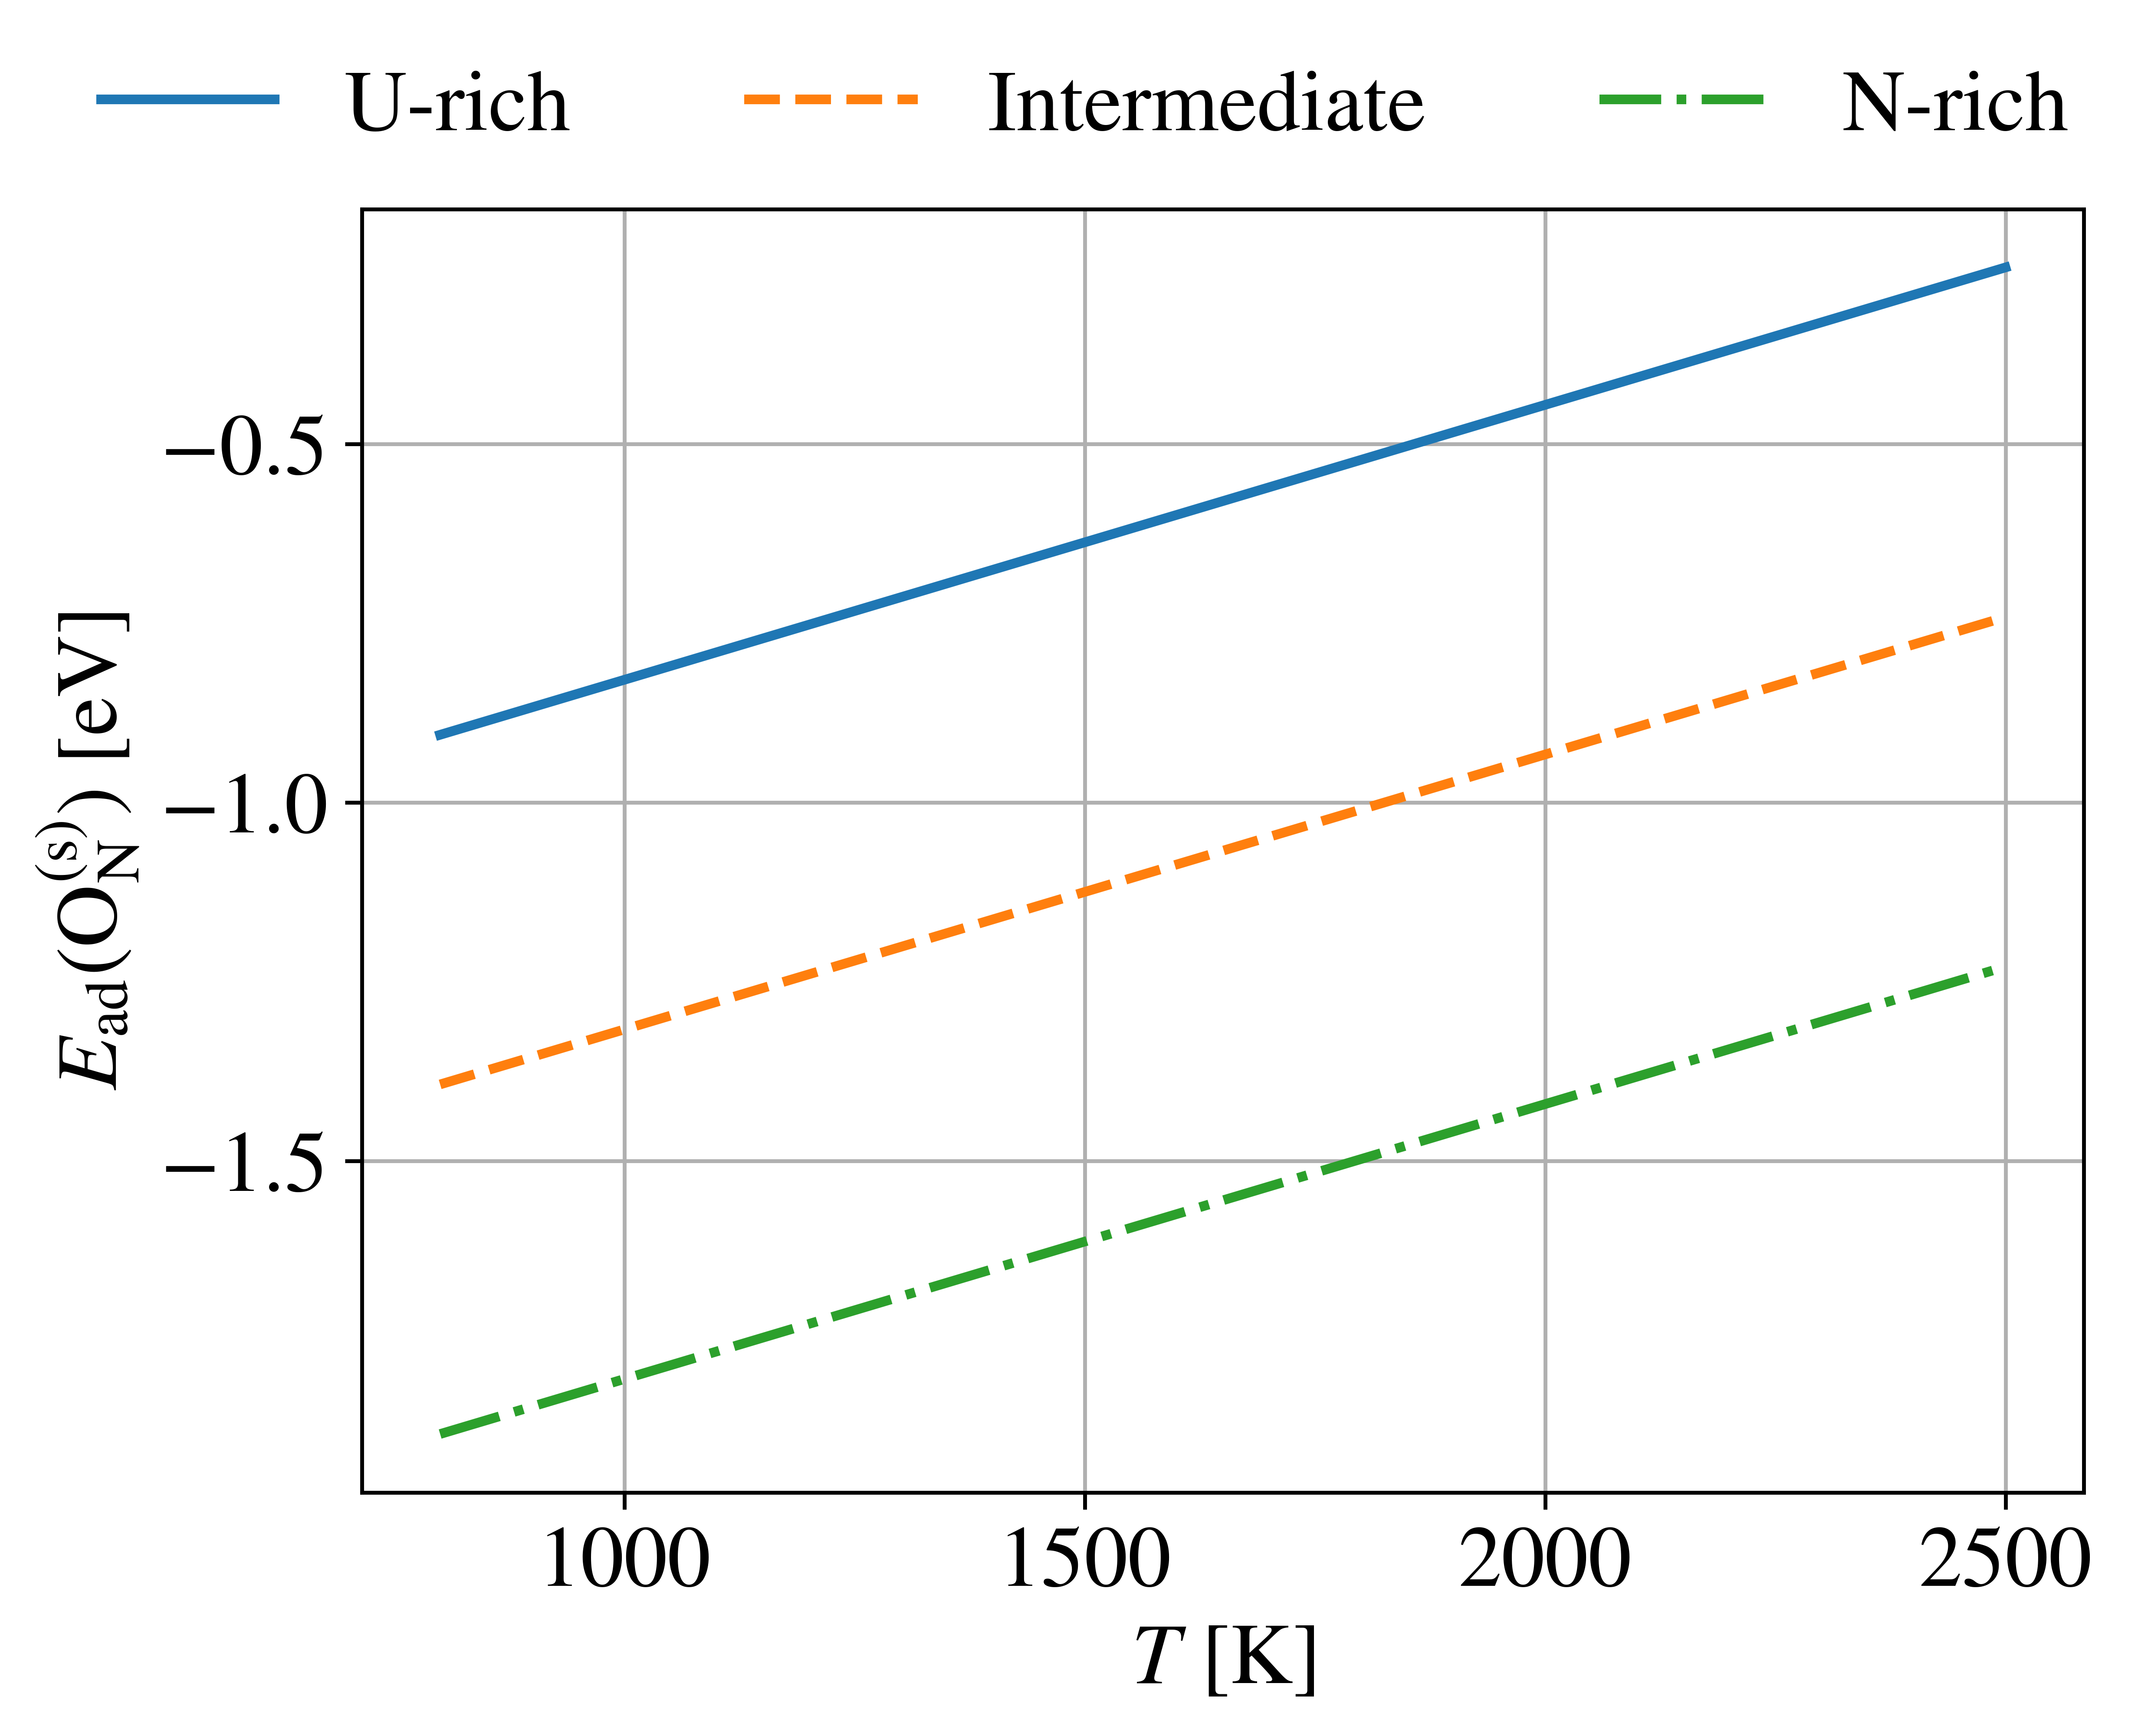
\includegraphics[width=\textwidth]{EadONs.png}
    \caption{}
    \label{Fig:EadONs}
\end{subfigure}
\hfill
\begin{subfigure}{0.48\textwidth}
    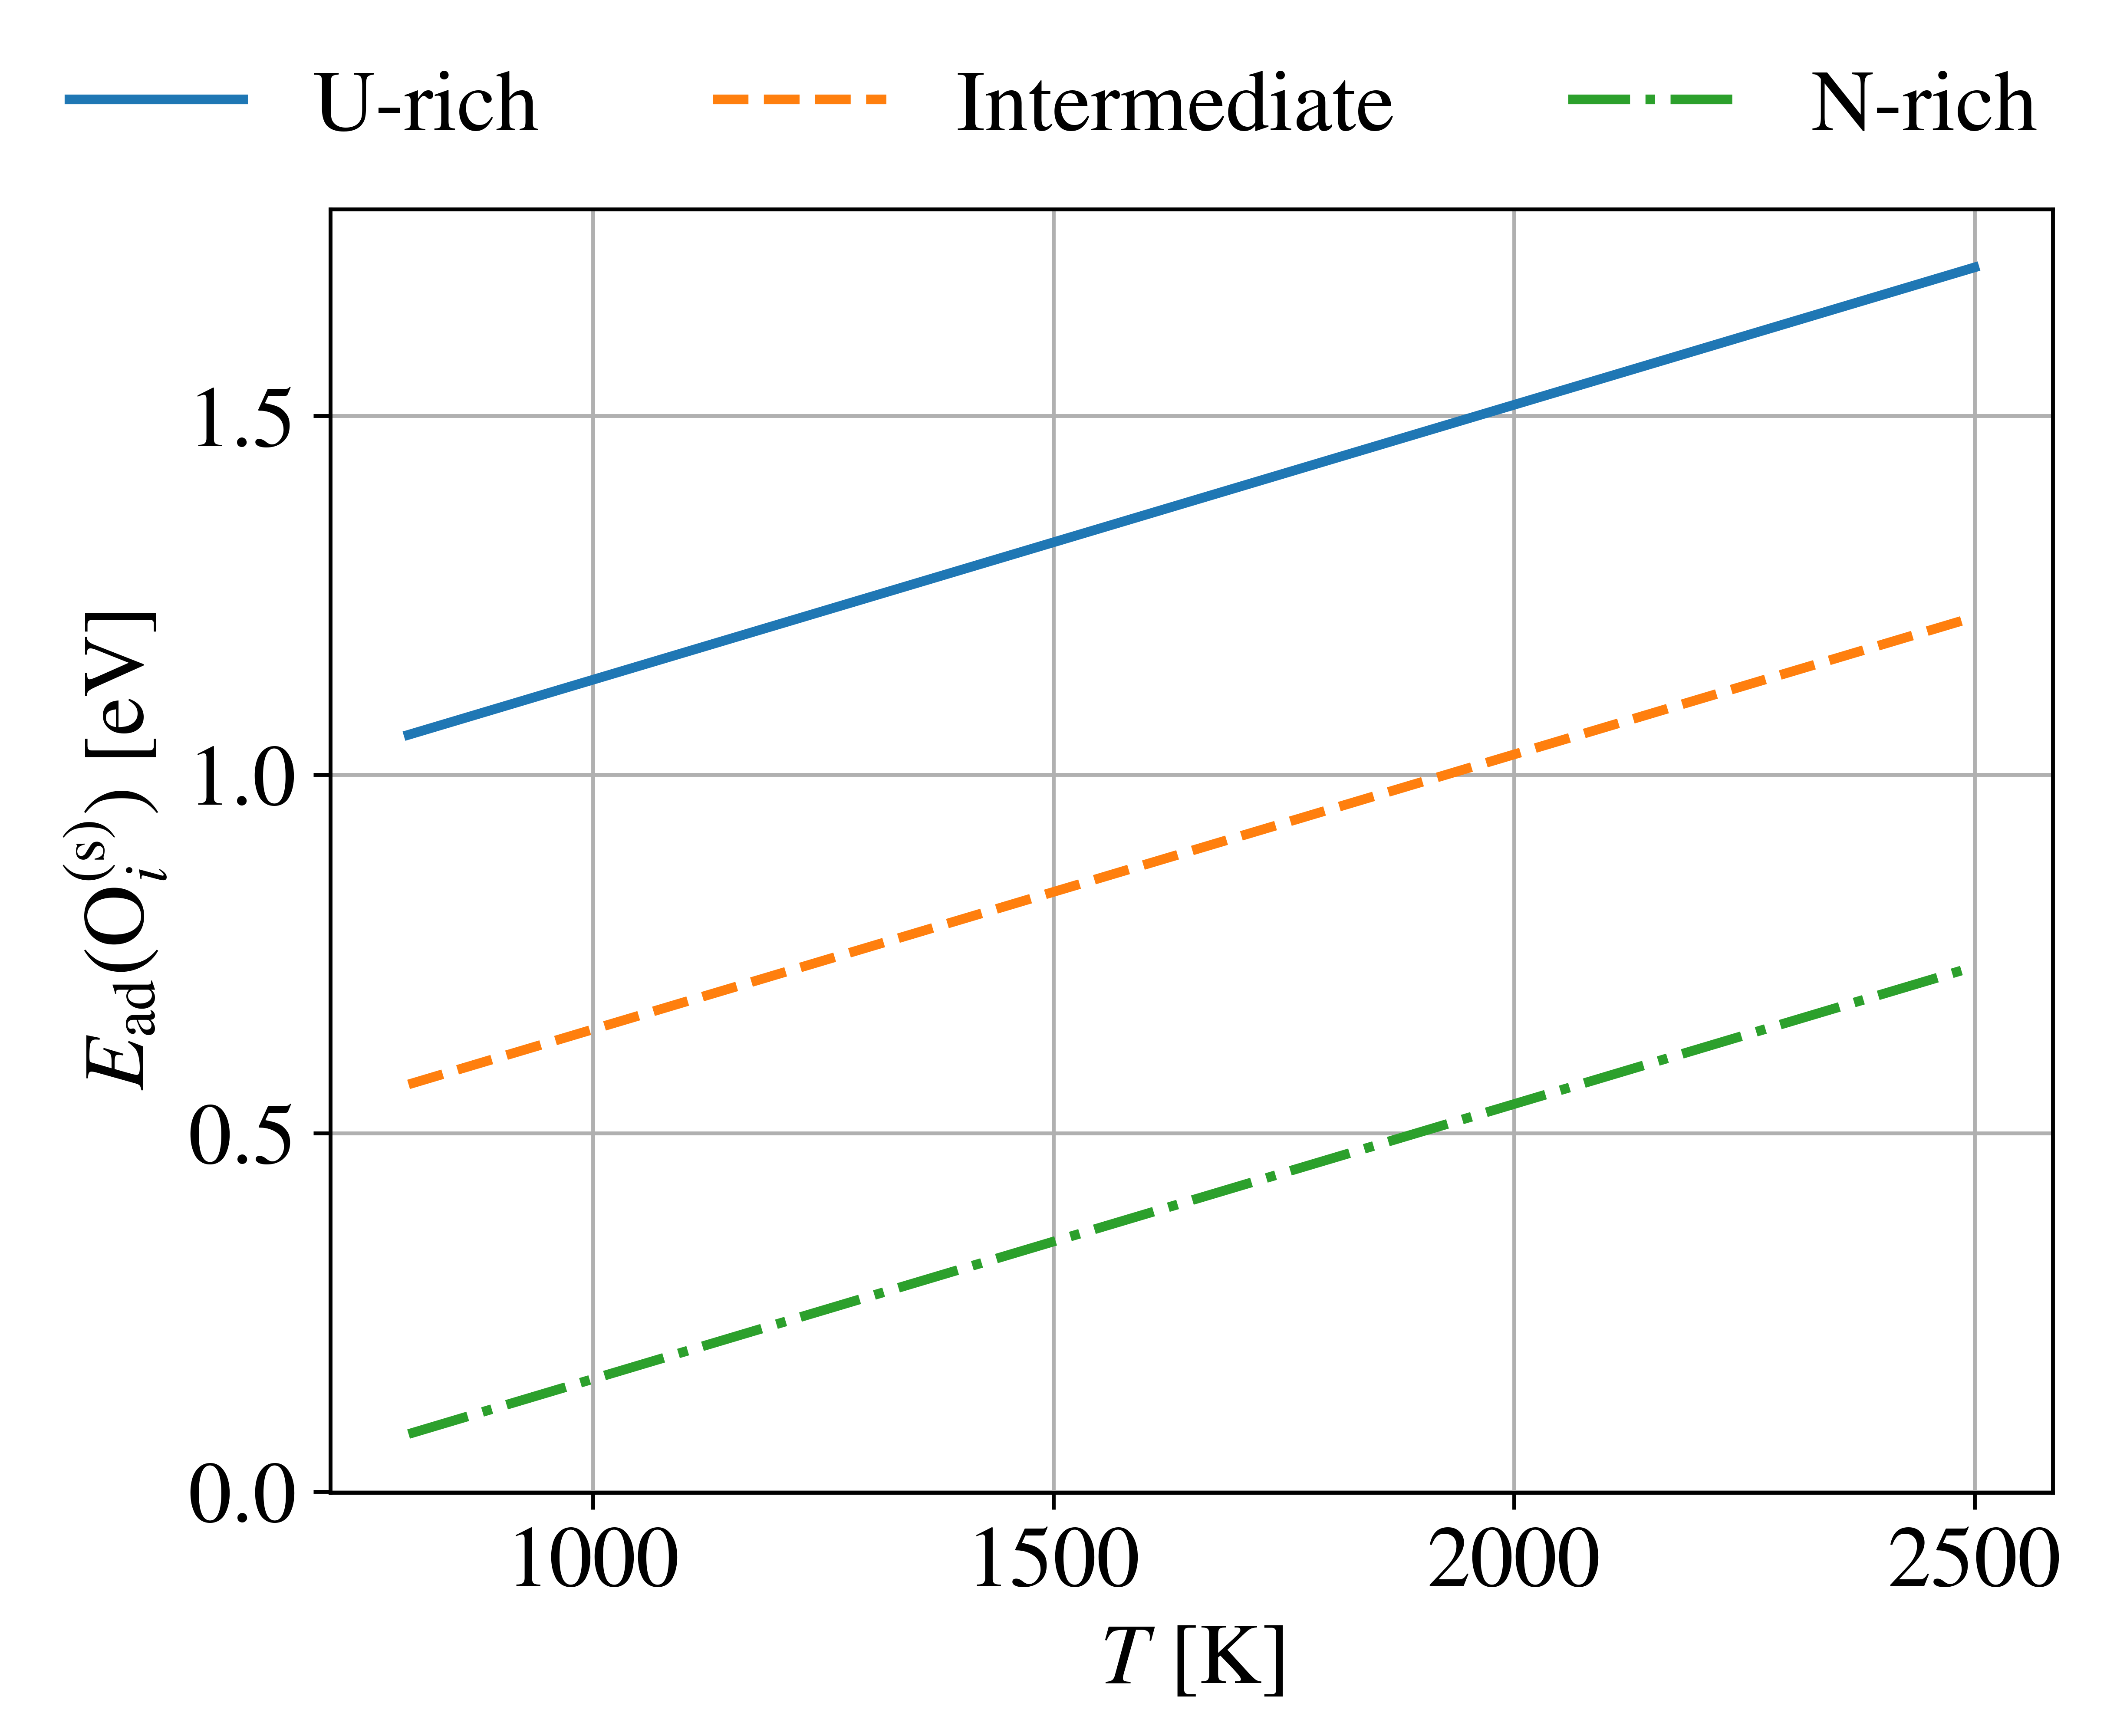
\includegraphics[width=\textwidth]{EadOis.png}
    \caption{}
    \label{Fig:EadOis}
\end{subfigure}
\caption{Temperature evolution of oxygen adsorption energy relative to the chemical potential shown in \cref{Fig:uO} for \textbf{(a)} $\text{O}_\text{N}^\text{(s)}$ and \textbf{(b)} $\text{O}_i^\text{(s)}$.}
\label{Fig:EduO}
\end{figure}

\subsection{Oxygen behavior}
\label{Sec:Oxygen}

Several parameters must be defined to study the behavior of oxygen using our model. We assume an initial oxygen concentration of $w_\text{O}$ = 1500 ppm, a porosity of $p$ = 5\%, and an average void radius of $R_v$ = 1 nm. The chosen $w_\text{O}$ = 1500 ppm is the upper limit of the tolerated oxygen impurity concentration in UN \cite{Rogozkin2003, Schuler2017}. The optimal initial (closed) porosity for UN fuels to both suppress oxidation and accommodate gaseous fission products is estimated to be 4\% \cite{Johnson2018}. Note that the porosity in irradiated fuels is typically as high as 15\% \cite{Nichenko2014}, which exceeds the 5\% porosity assumed here. Lastly, the lower limit of reported fission gas bubble sizes in nitride and carbide fuels is close to $R_v$ = 1 nm \cite{Matzke1986}, which is also the critical void radius in metals \cite{Zinkle1987b}.

The atomic concentrations of the N vacancy in the bulk and on the void surfaces are calculated with the aid of formation energies in \cref{Tab:EfVN} and \cref{Eq:VN-VNs} and are shown in \cref{Fig:VN,Fig:VNs}, respectively. The concentrations of $\text{O}_i^\text{(b)}$ and $\{\text{O}_\text{N} \! : \! v_\text{N}\}^\text{(b)}$, relative to $\text{O}_\text{N}^\text{(b)}$ are shown in \cref{Fig:Oi_ON,Fig:ONVN_ON}, respectively. It is clear that $\text{O}_\text{N}^\text{(b)}$ is the dominant defect type for oxygen impurities. Thus, it is justified to set $[ \text{O}_\text{N}^\text{(b)} ] \approx c_\text{O}$ where $c_\text{O}$ is the atomic fraction of oxygen impurities, given by \cref{Eq:cO}. $\text{O}_\text{N}^\text{(b)}$ is an immobile defect. Surface energy reduction requires O migration to void surfaces, which can only occur via the mobile defects $\text{O}_i^\text{(b)}$ and $\{\text{O}_\text{N} \! : \! v_\text{N}\}^\text{(b)}$. However, the immobile $\text{O}_\text{N}^\text{(b)}$ defects can stabilize void embryos via another mechanism by binding to $v_\text{U}$, $\text{Kr}_\text{U}$, and $\text{Xe}_\text{U}$, as explained earlier.
 
\begin{figure}[h!]
\centering
\begin{subfigure}{0.48\textwidth}
    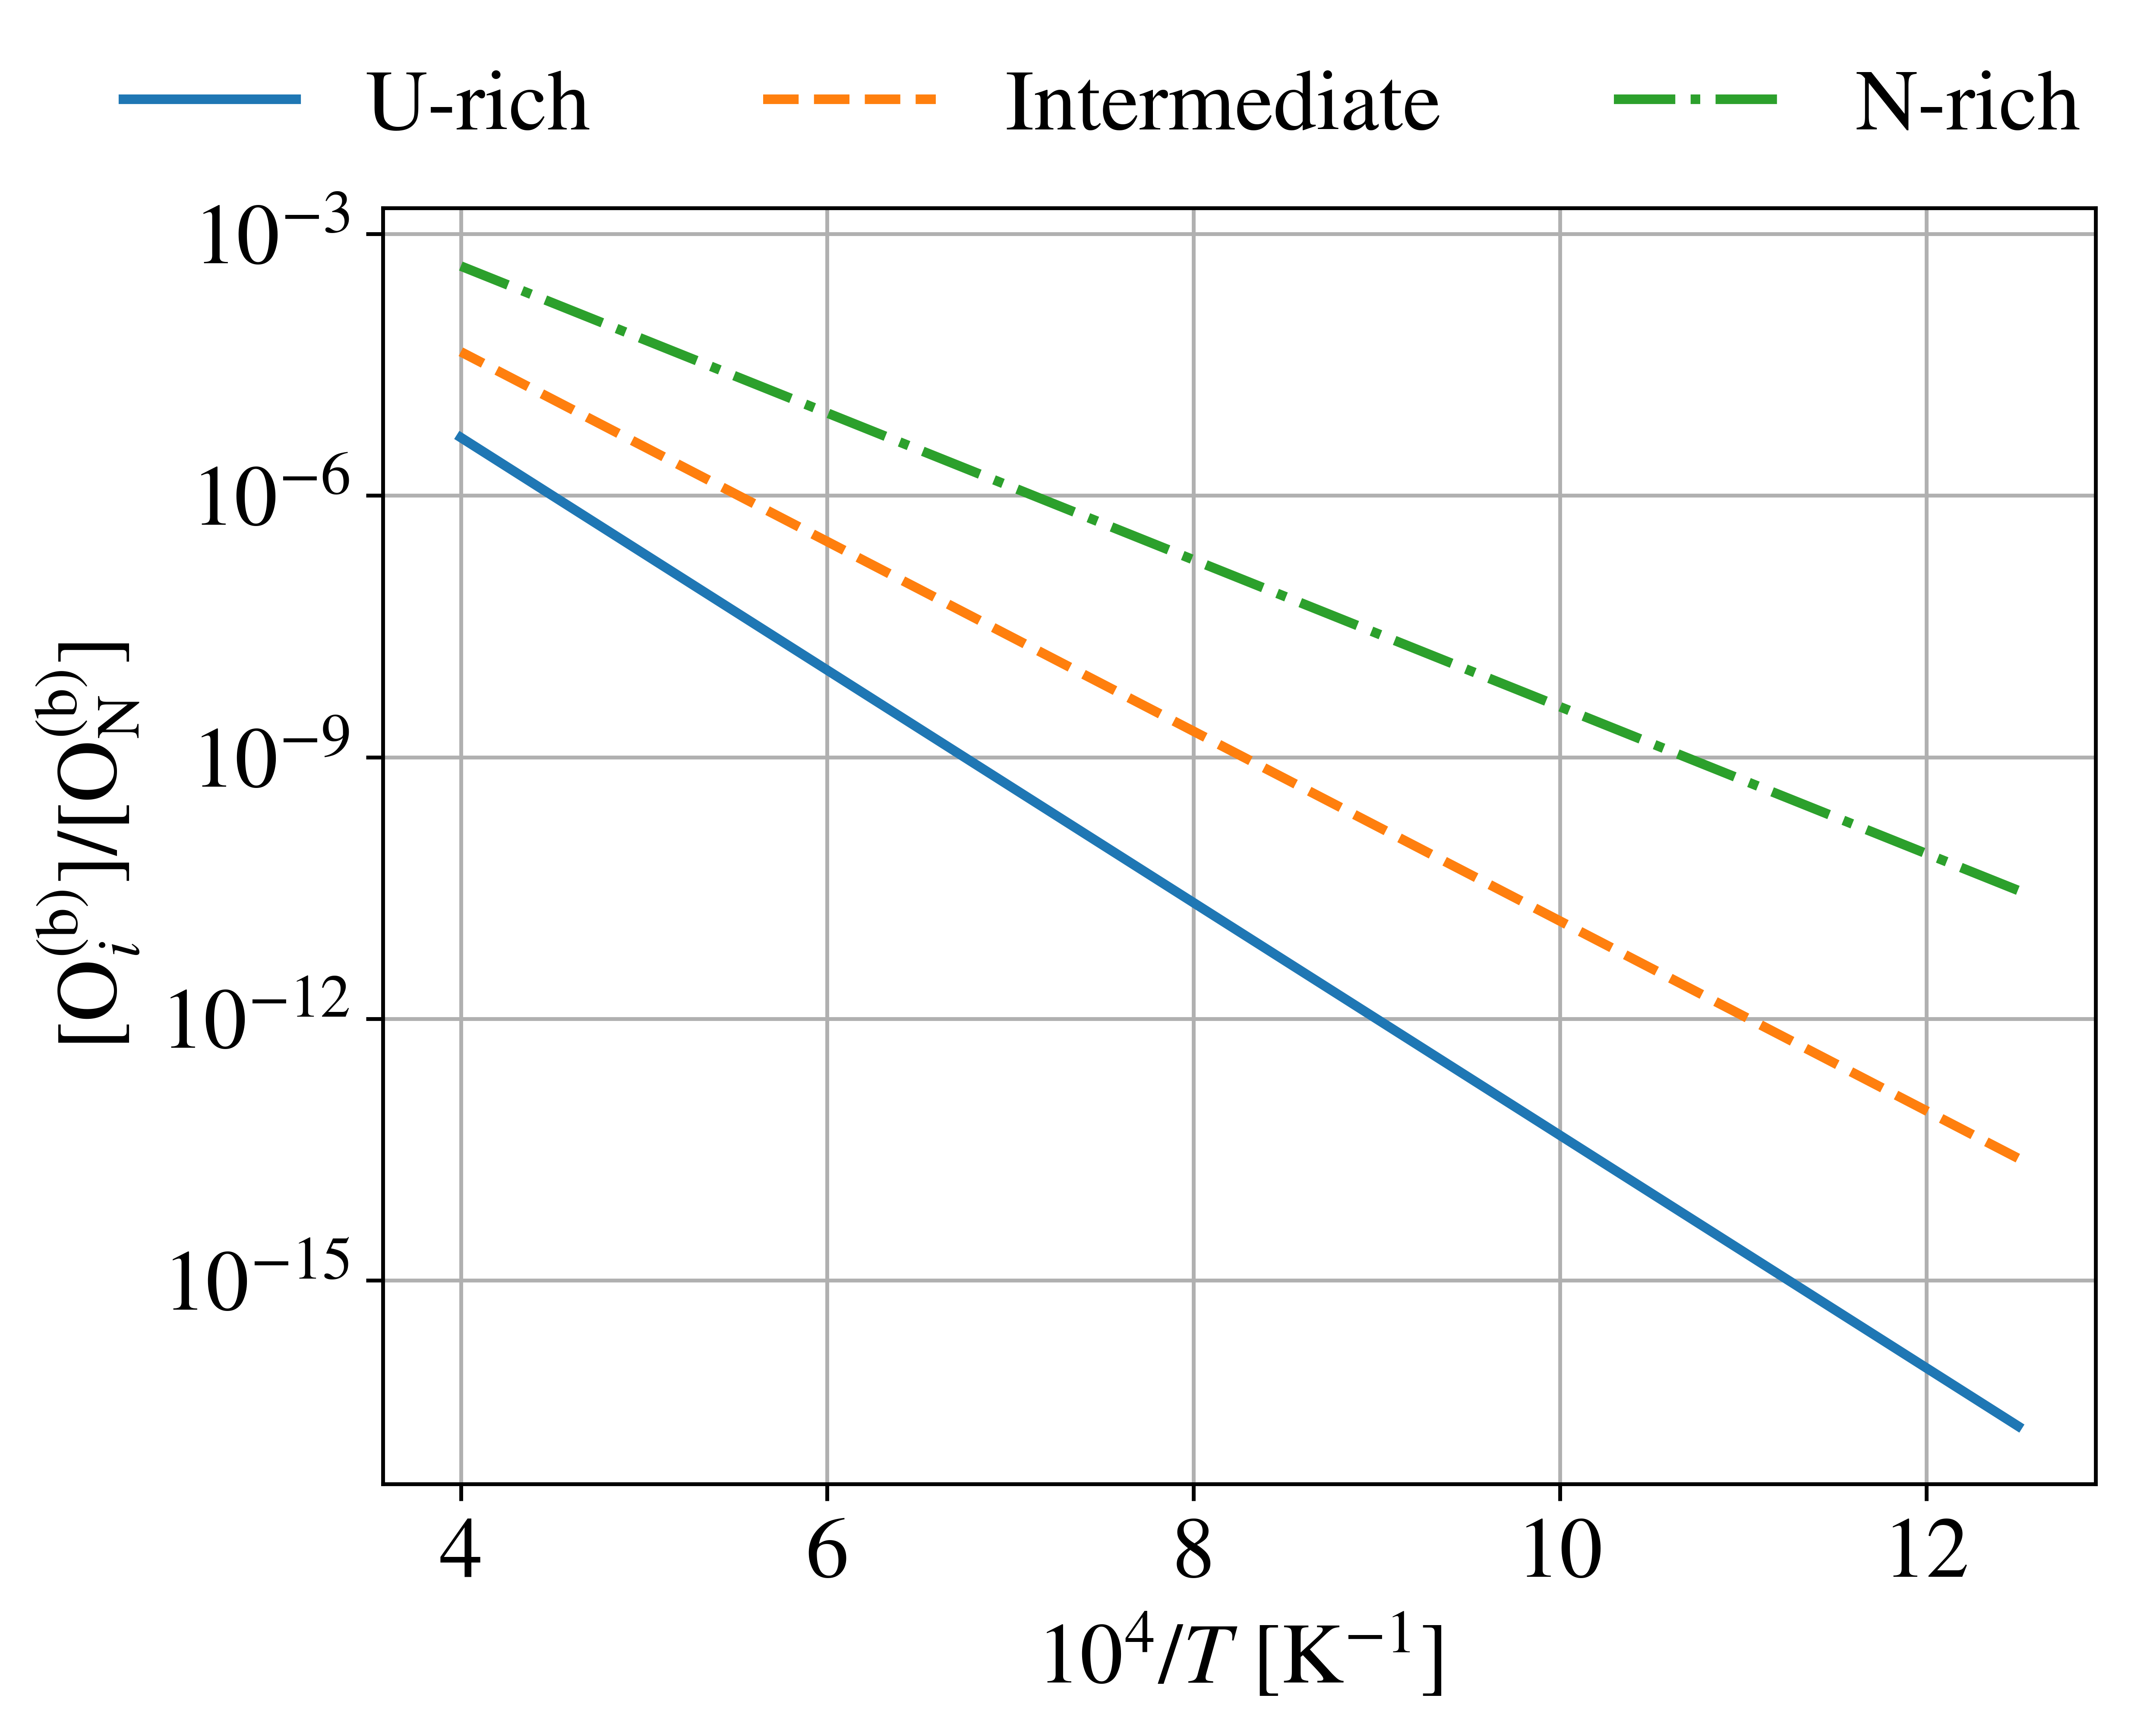
\includegraphics[width=\textwidth]{Oi_ON.png}
    \caption{}
    \label{Fig:Oi_ON}
\end{subfigure}
\hfill
\begin{subfigure}{0.48\textwidth}
    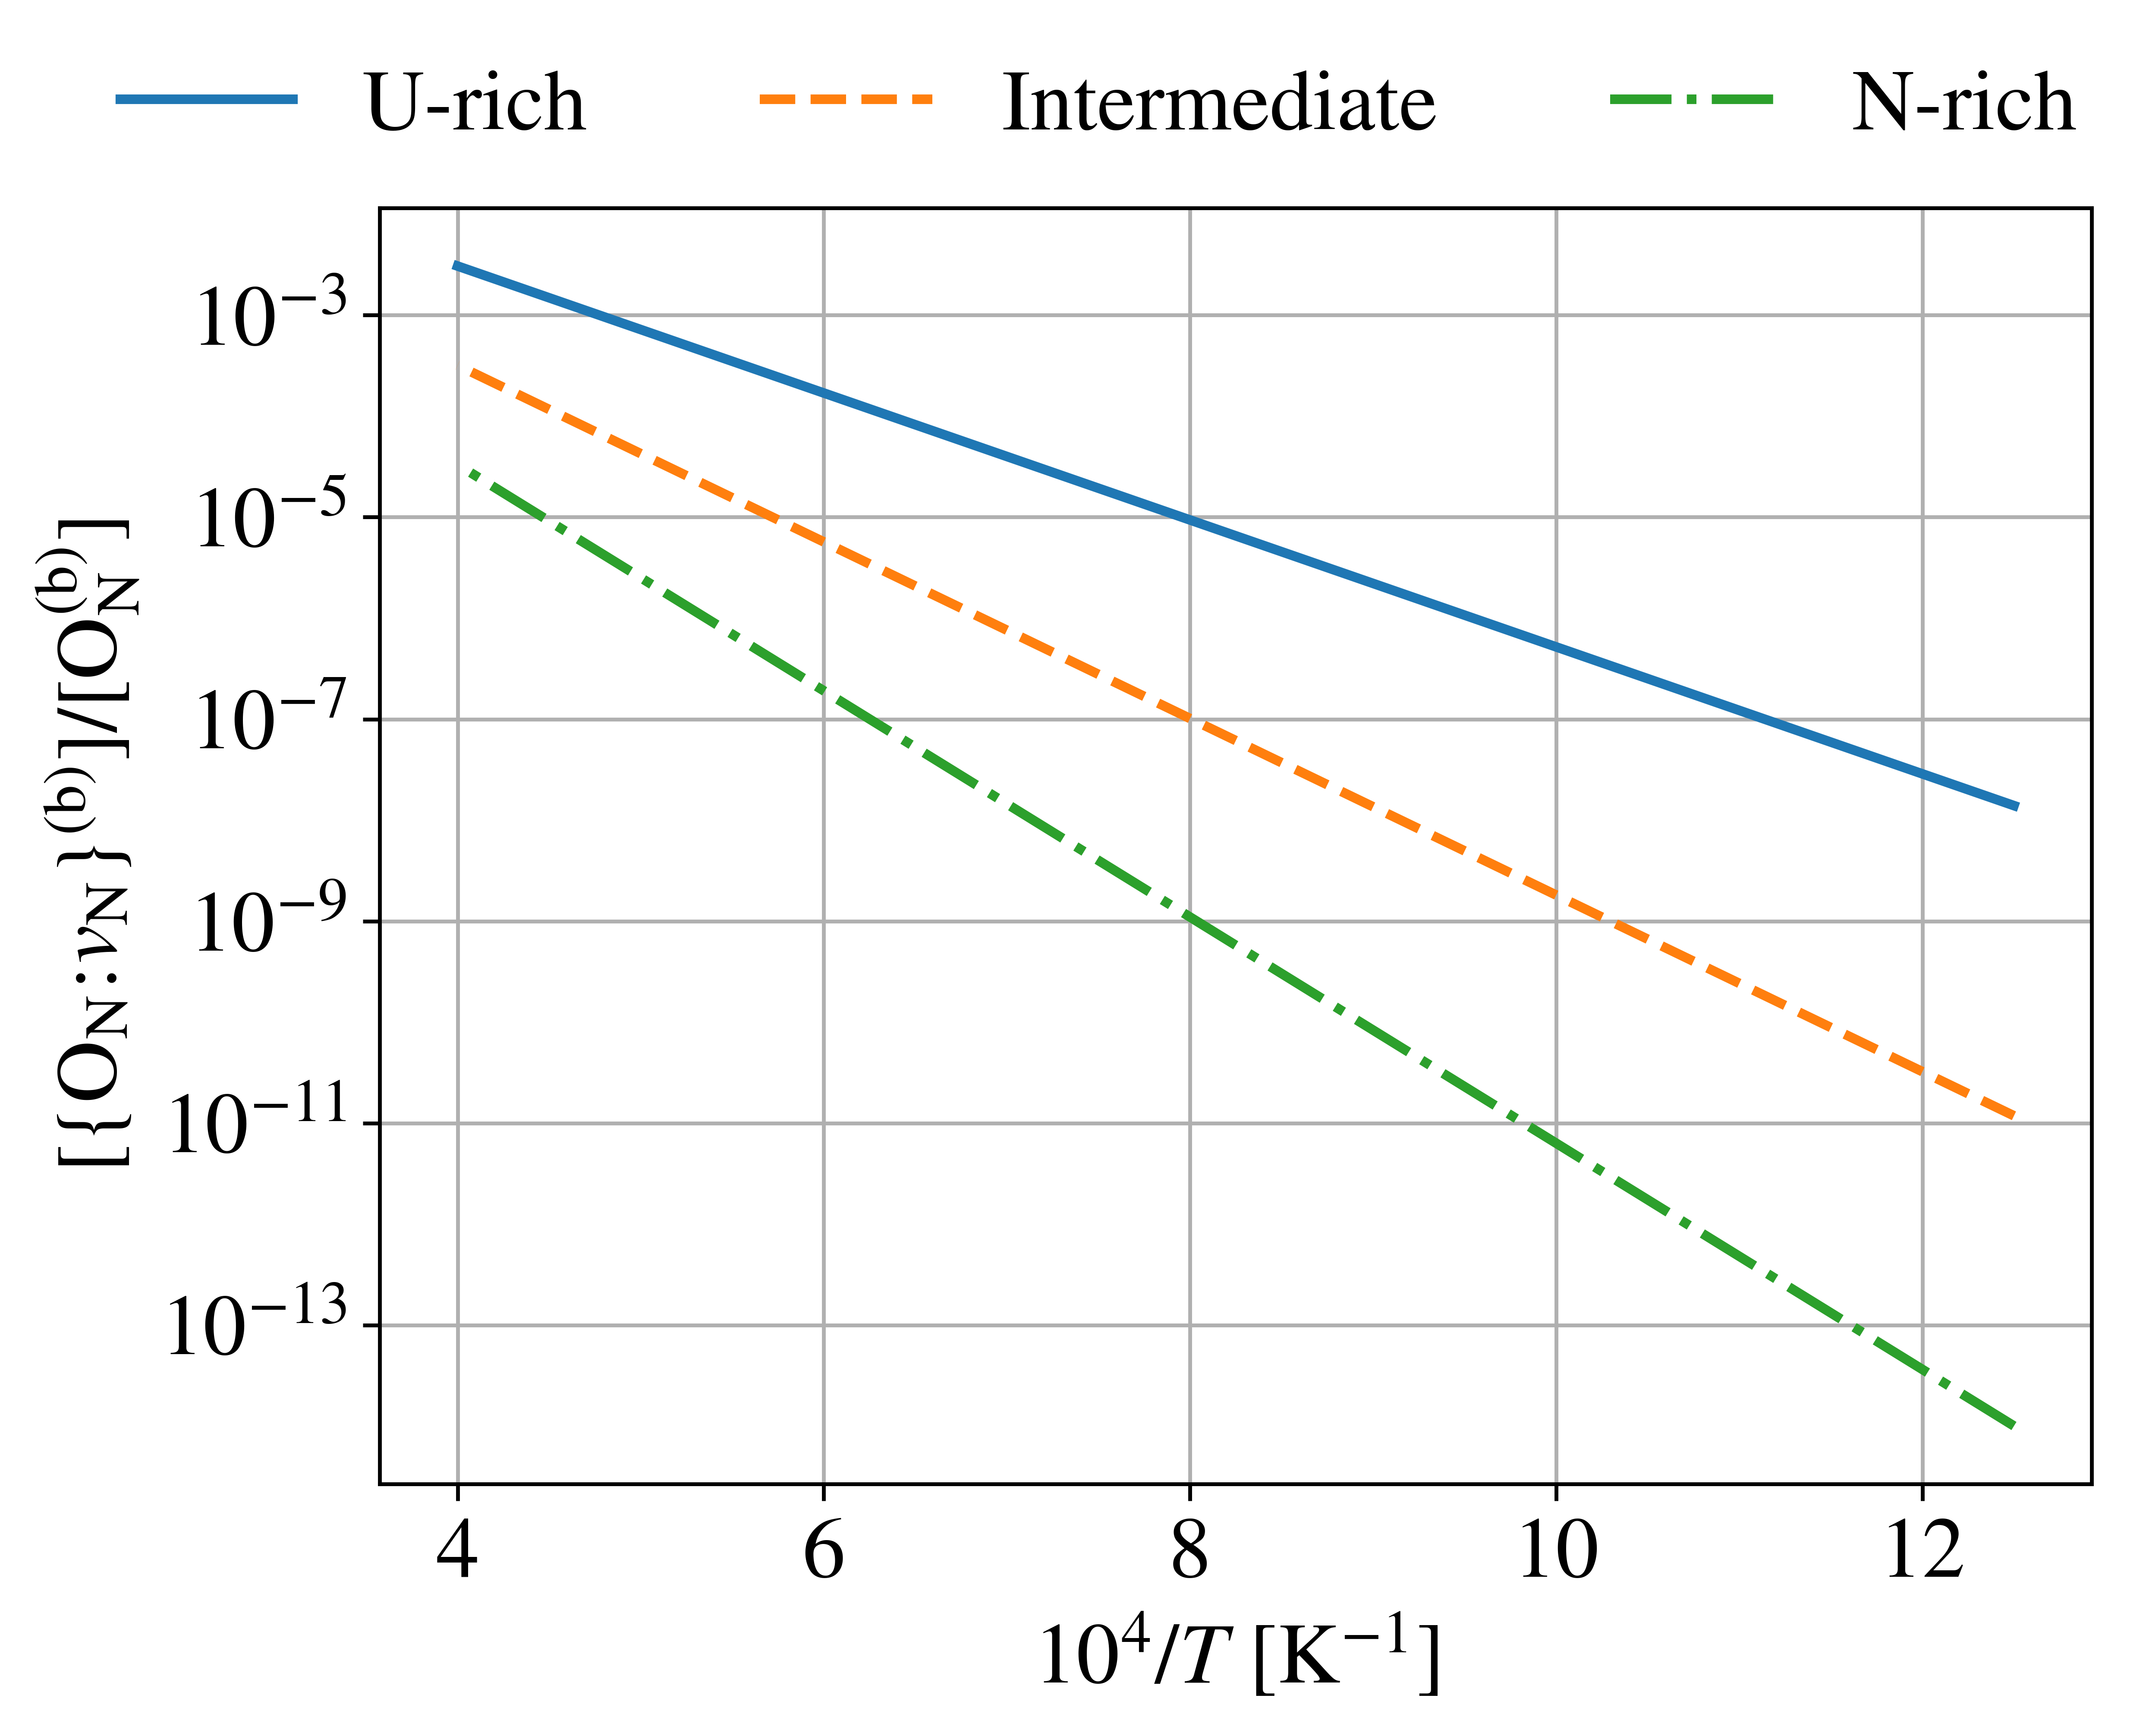
\includegraphics[width=\textwidth]{ONVN_ON.png}
    \caption{}
    \label{Fig:ONVN_ON}
\end{subfigure}
\caption{Relative concentrations of \textbf{(a)} $\text{O}_i^\text{(b)}$ and \textbf{(b)} $\{\text{O}_\text{N} \! : \! v_\text{N}\}^\text{(b)}$.}
\label{2}
\end{figure}

The relative concentration $ [ \text{O}_i^\text{(s)} ] / [ \text{O}_\text{N}^\text{(b)} ] $ is illustrated in \cref{Fig:Ois_ONb}. Under U-rich and intermediate conditions, this relative concentration exhibits Arrhenius behavior and remains relatively low. However, under N-rich conditions, which are more relevant in irradiation environments, the relative concentration is significantly higher and follows an anti-Arrhenius trend. Around 1600 K, for instance, for every ten oxygen atoms in the bulk, approximately one oxygen atom segregates to the surface as $ \text{O}_i^\text{(s)} $. This behavior arises because, in N-rich environments, there are fewer nitrogen vacancies available to form $ \text{O}_\text{N}^\text{(s)} $, leading to a preference for oxygen atoms to segregate to the surface. Similarly, in \cref{Fig:ONs_ONb}, an anti-Arrhenius trend is also observed for the relative concentration $ [ \text{O}_\text{N}^\text{(s)} ] / [ \text{O}_\text{N}^\text{(b)} ] $. This behavior is independent of stoichiometry, as it is solely governed by the segregation energy. As expected, this anti-Arrhenius behavior indicates that the solubility of oxygen in the bulk increases with increasing temperature. Lastly, \cref{Fig:Ois_ONs} depicts the relative concentration $ [ \text{O}_i^\text{(s)} ] / [ \text{O}_\text{N}^\text{(s)} ] $. As expected, $ \text{O}_\text{N}^\text{(s)} $ is the dominant oxygen impurity site on the void surfaces. Interestingly, despite the large difference in adsorption energies, this relative concentration exceeds 0.1 in N-rich conditions across all considered temperatures.

% At very low temperatures, this ratio exceeds 1, meaning that, if kinetic limitations were to be neglected, for every oxygen atom in the bulk, approximately two atoms would segregate to the surface as $ \text{O}_\text{N}^\text{(s)} $.

\begin{figure}[h!]
\centering
\begin{subfigure}{0.48\textwidth}
    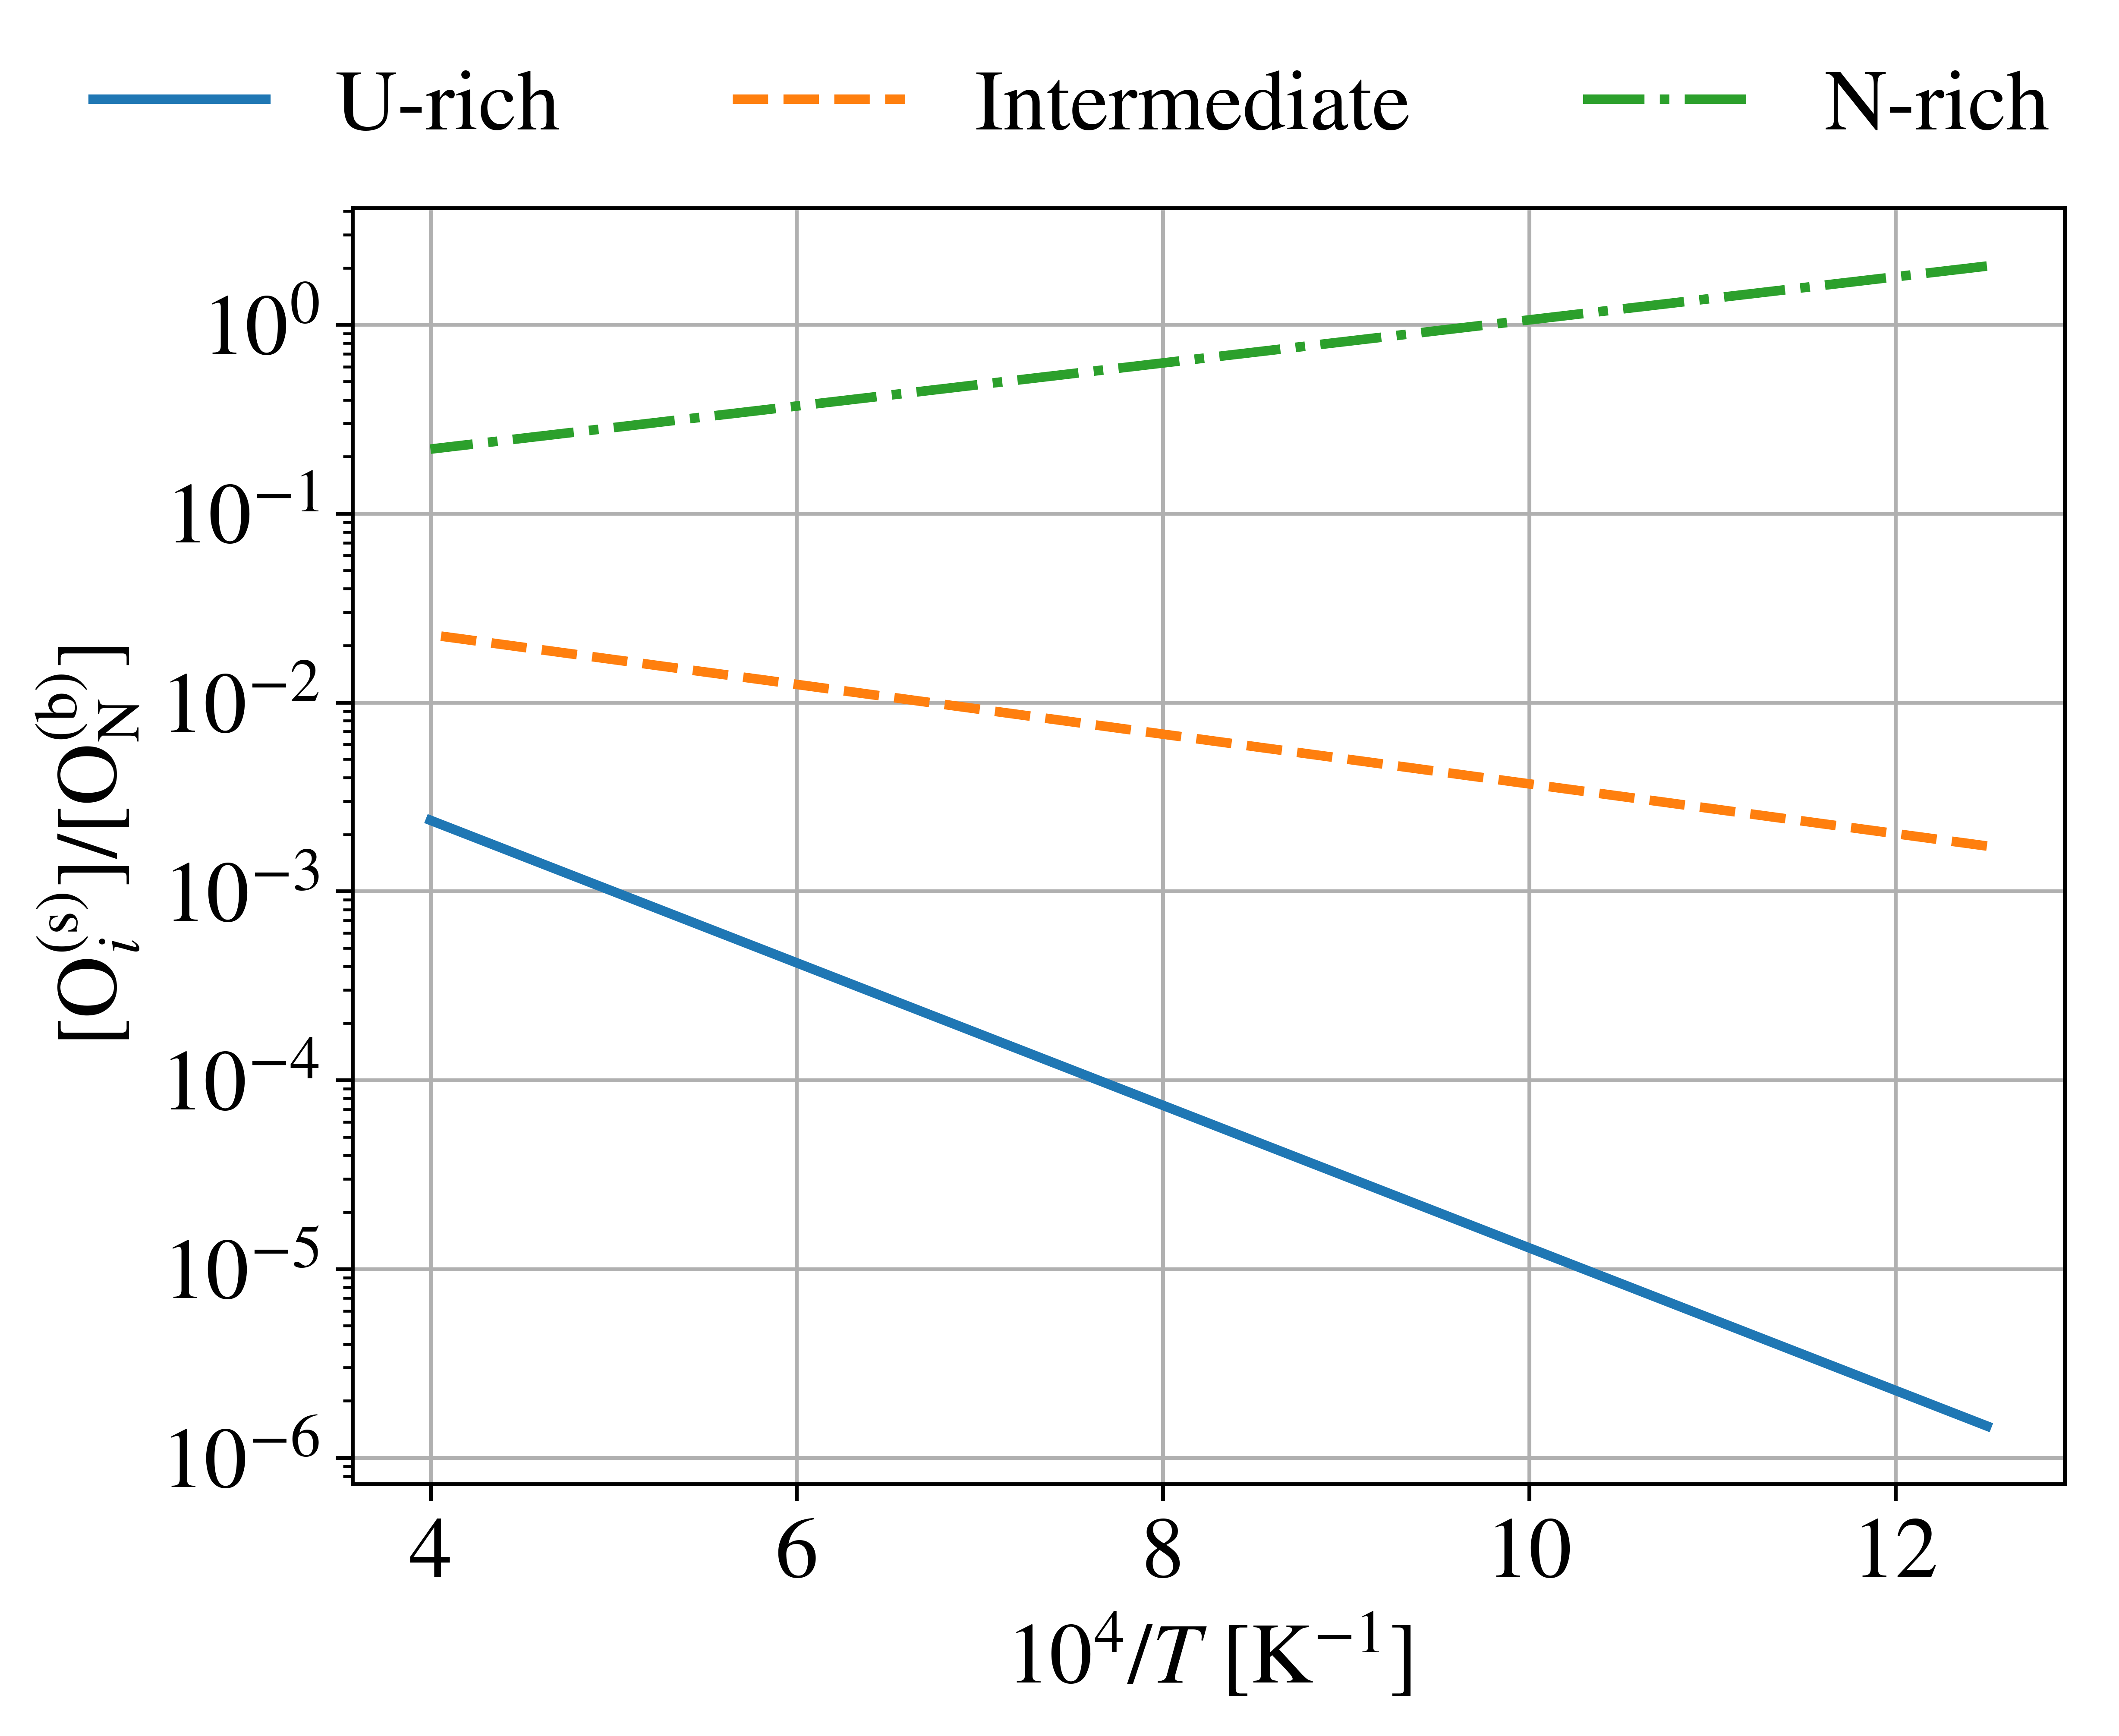
\includegraphics[width=\textwidth]{Ois_ONb.png}
    \caption{}
    \label{Fig:Ois_ONb}
\end{subfigure}
\hfill
\begin{subfigure}{0.48\textwidth}
    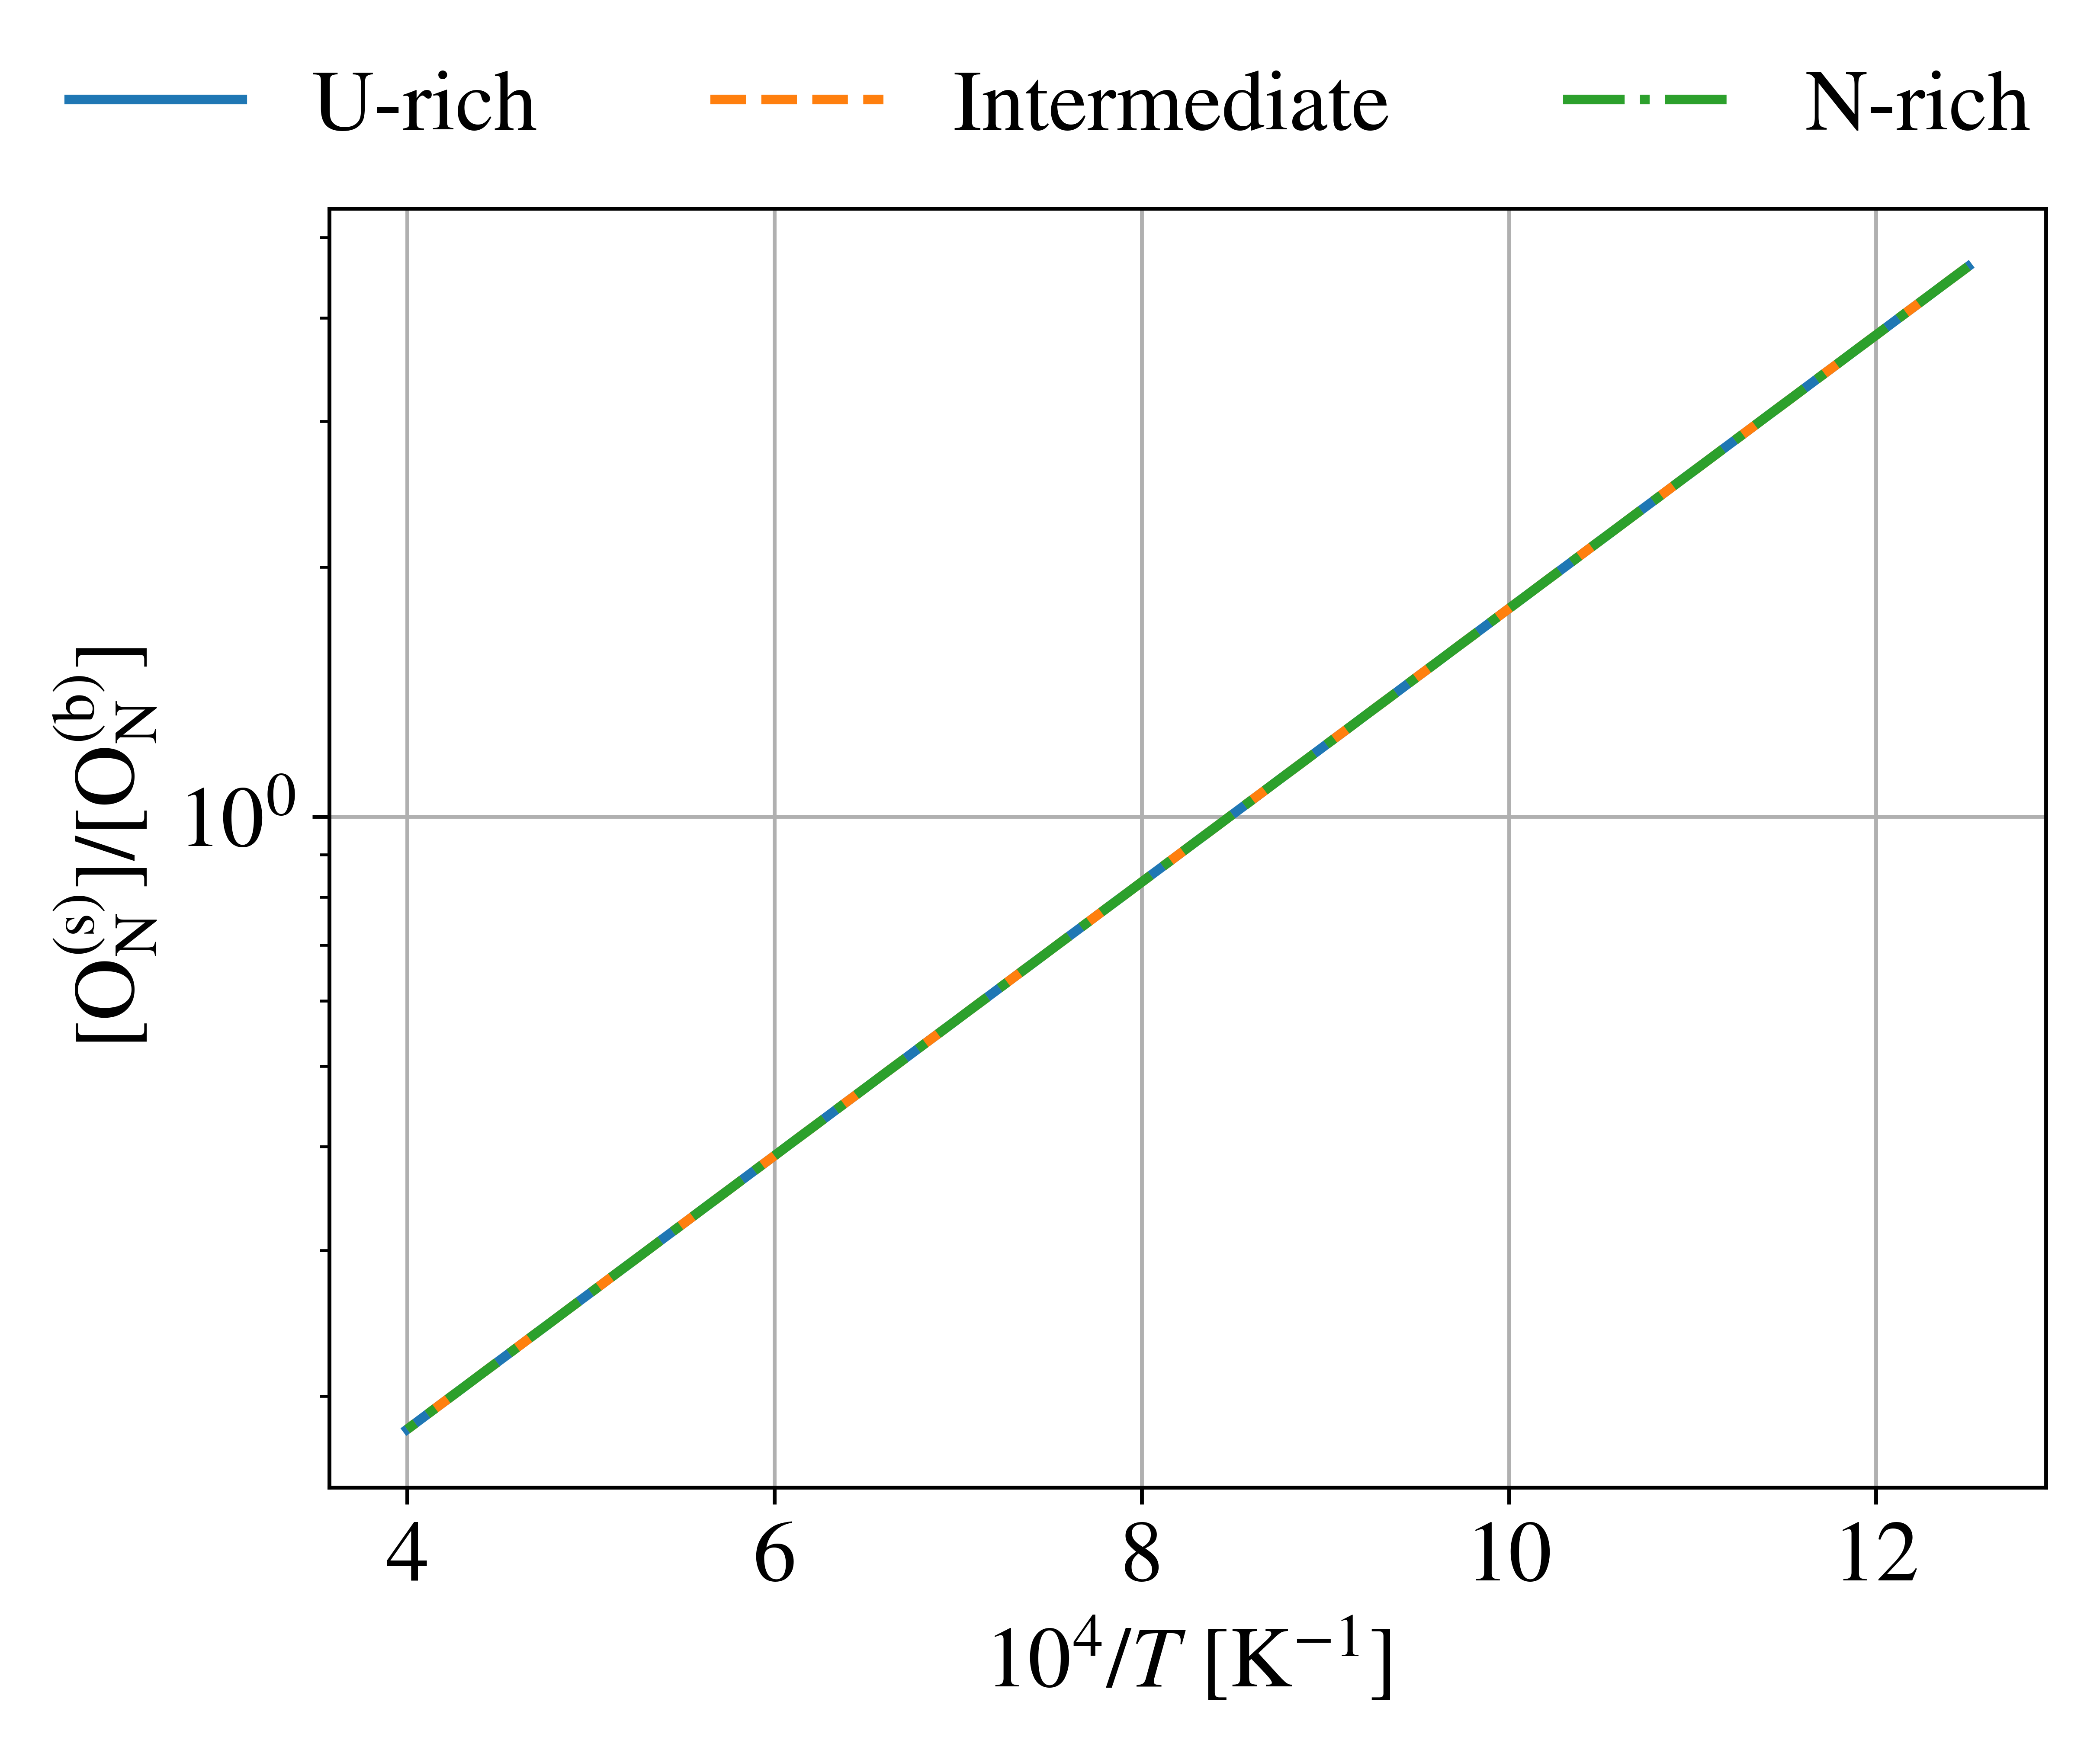
\includegraphics[width=\textwidth]{ONs_ONb.png}
    \caption{}
    \label{Fig:ONs_ONb}
\end{subfigure}
\hfill
\begin{subfigure}{0.48\textwidth}
    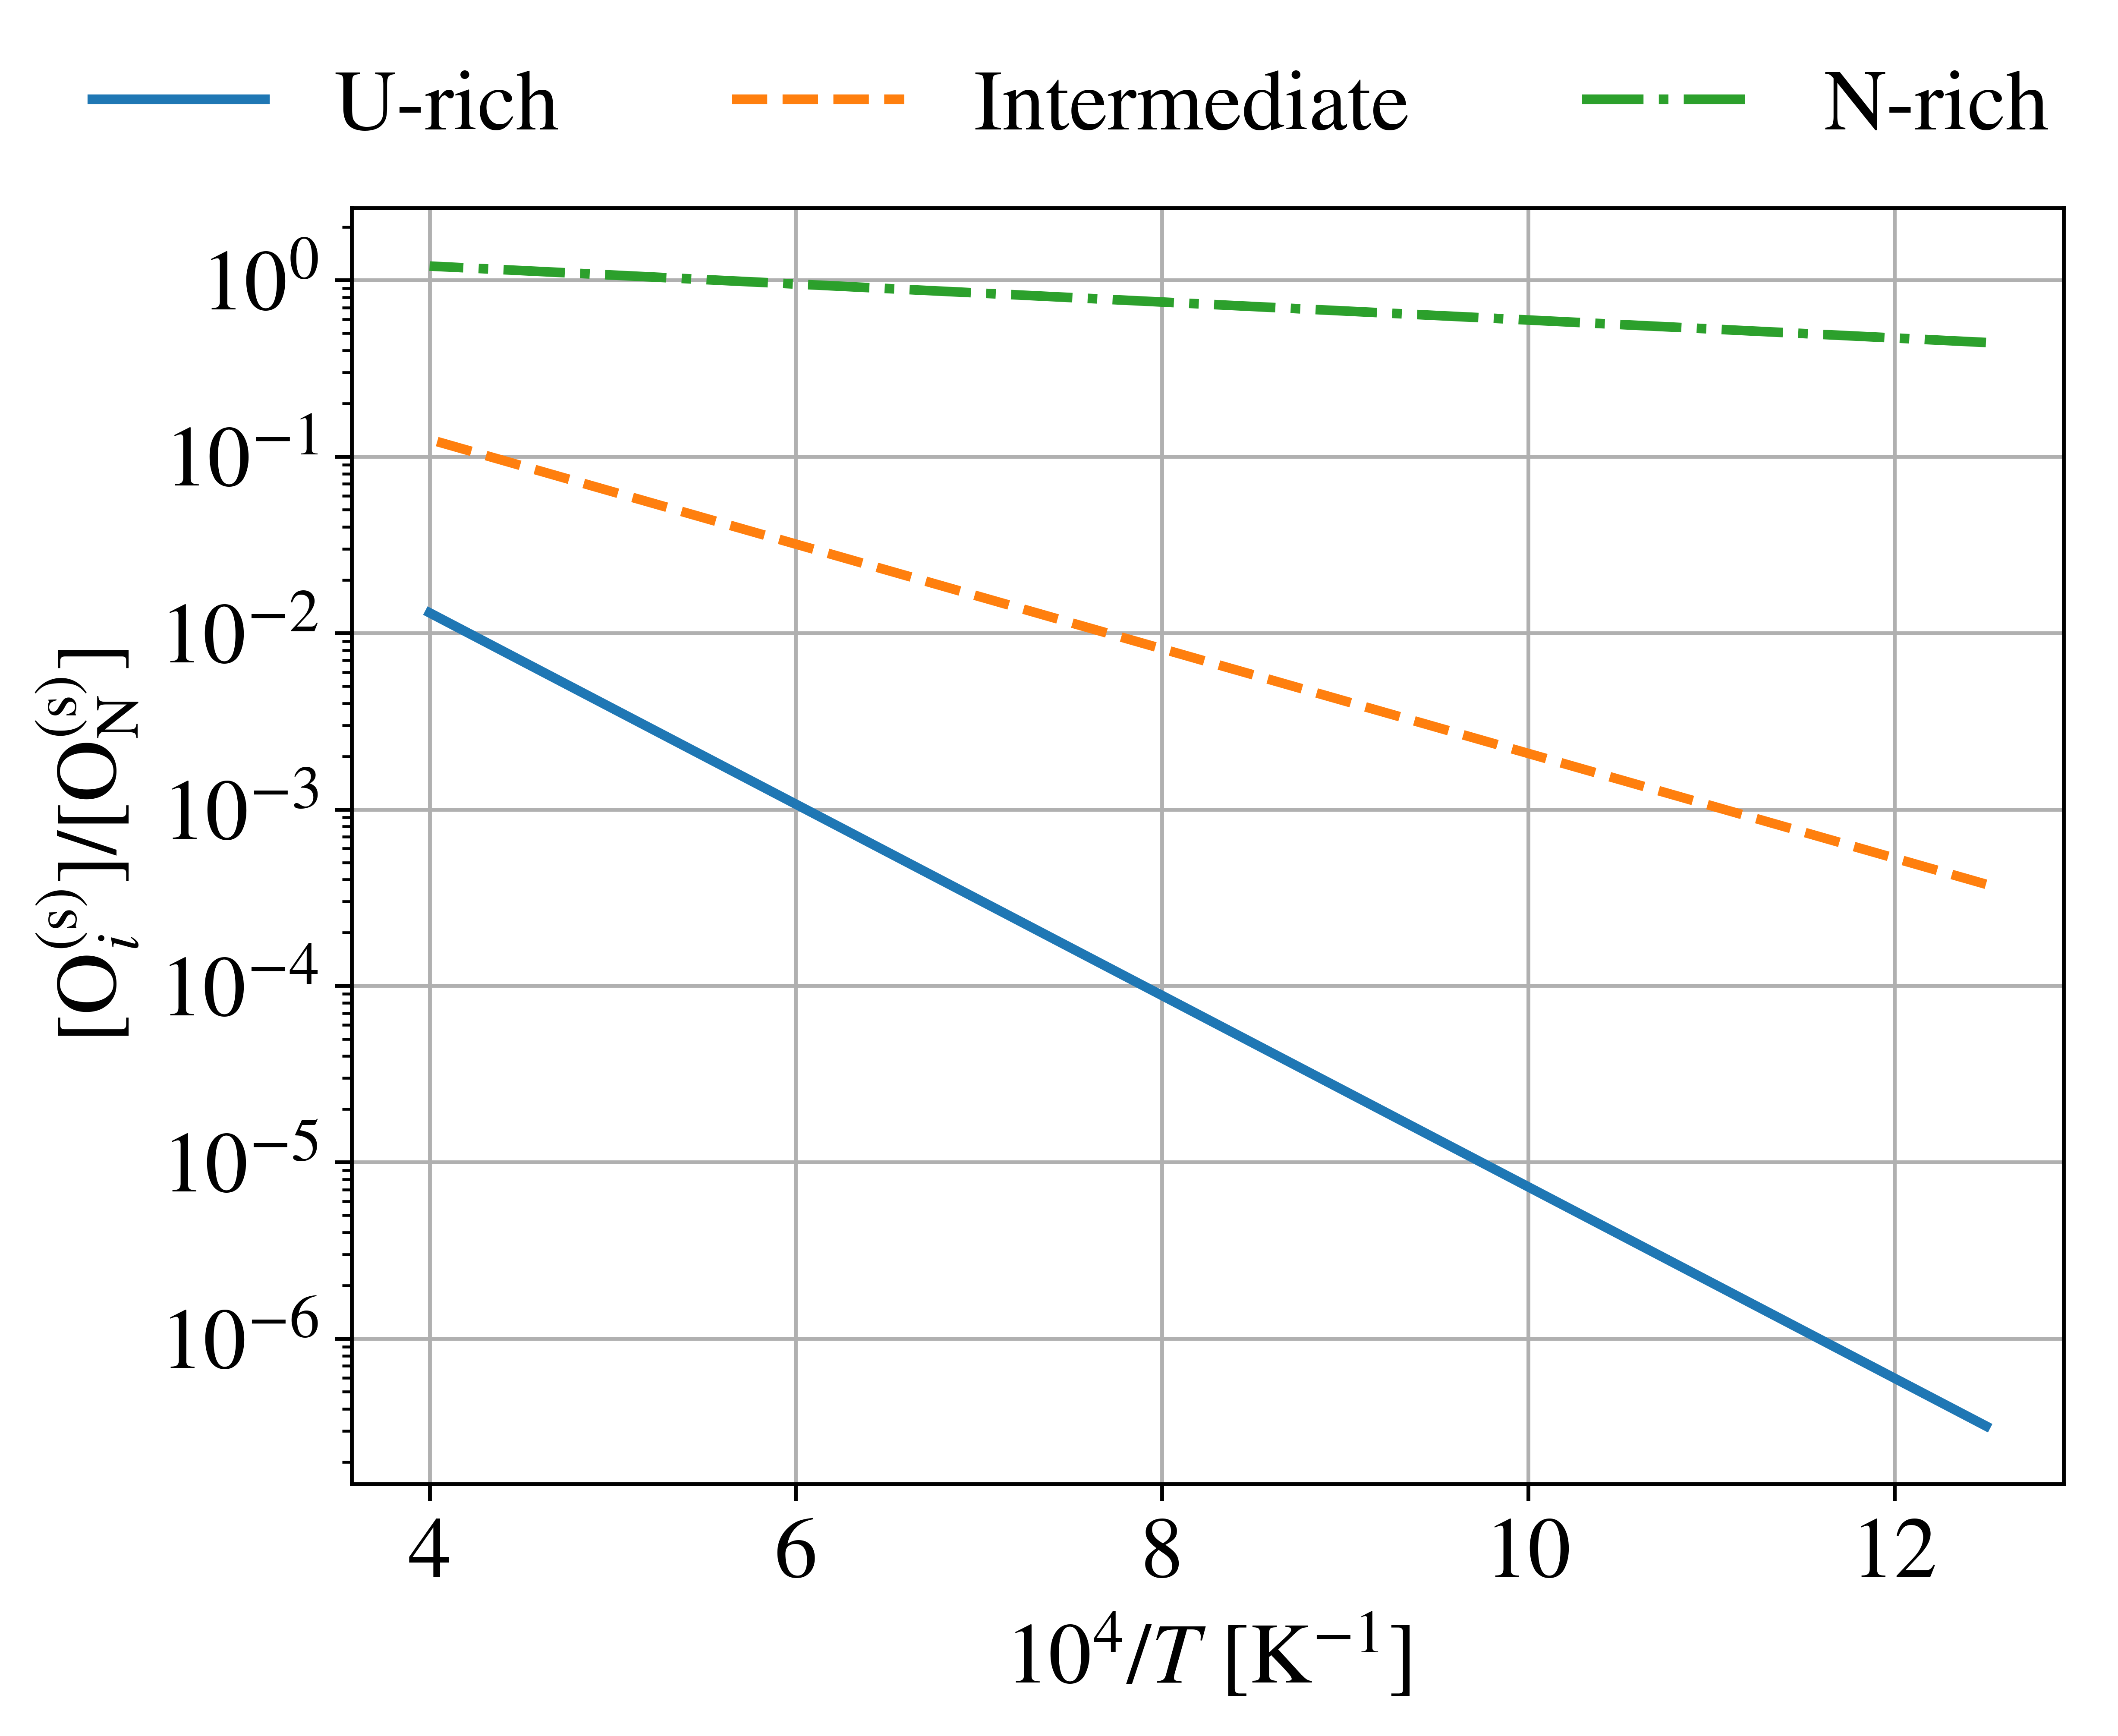
\includegraphics[width=\textwidth]{Ois_ONs.png}
    \caption{}
    \label{Fig:Ois_ONs}
\end{subfigure}
\caption{Relative concentrations of \textbf{(a)} $\text{O}_i^\text{(s)}$ and \textbf{(b)} $\text{O}_\text{N}^\text{(s)}$, as well as \textbf{(c)} the ratio of their concentrations.}
\label{3}
\end{figure}

The diffusivity of oxygen impurities in bulk UN through mechanisms dependent on the $\{\text{O}_\text{N} \! : \! v_\text{N}\}$ and $\text{O}_i$ defects is illustrated in \cref{Fig:DO}. Under U-rich conditions, the defect cluster $ \{\text{O}_\text{N} \! : \! v_\text{N}\} $ dominates oxygen diffusion. This can be explained by the fact that U-rich environments have a higher concentration of nitrogen vacancies, allowing oxygen to exist as $ \text{O}_\text{N} $ in the bulk. These nitrogen vacancies also facilitate the diffusion process. In intermediate conditions, both diffusion mechanisms are comparable, although $ \text{O}_i $ exhibits slightly higher diffusivity. In contrast, under N-rich conditions, the availability of nitrogen vacancies decreases, and oxygen predominantly exists as an interstitial $ \text{O}_i $. Consequently, the diffusion mechanism via $ \text{O}_i $ becomes dominant in this regime.

It is important to note that we assume $ \text{O}_\text{N}^\text{(s)} $ defects reach the surface predominantly through the diffusion of $ \{\text{O}_\text{N} \! : \! v_\text{N}\} $. This assumption is later utilized when calculating the reduction in surface energy due to surface adsorption. Specifically, the diffusivity used to calculate $\alpha_1$ in \cref{Eq:DeltaSigma1} is that of $ \{\text{O}_\text{N} \! : \! v_\text{N}\} $.

\begin{figure}[h!]
    \centering
    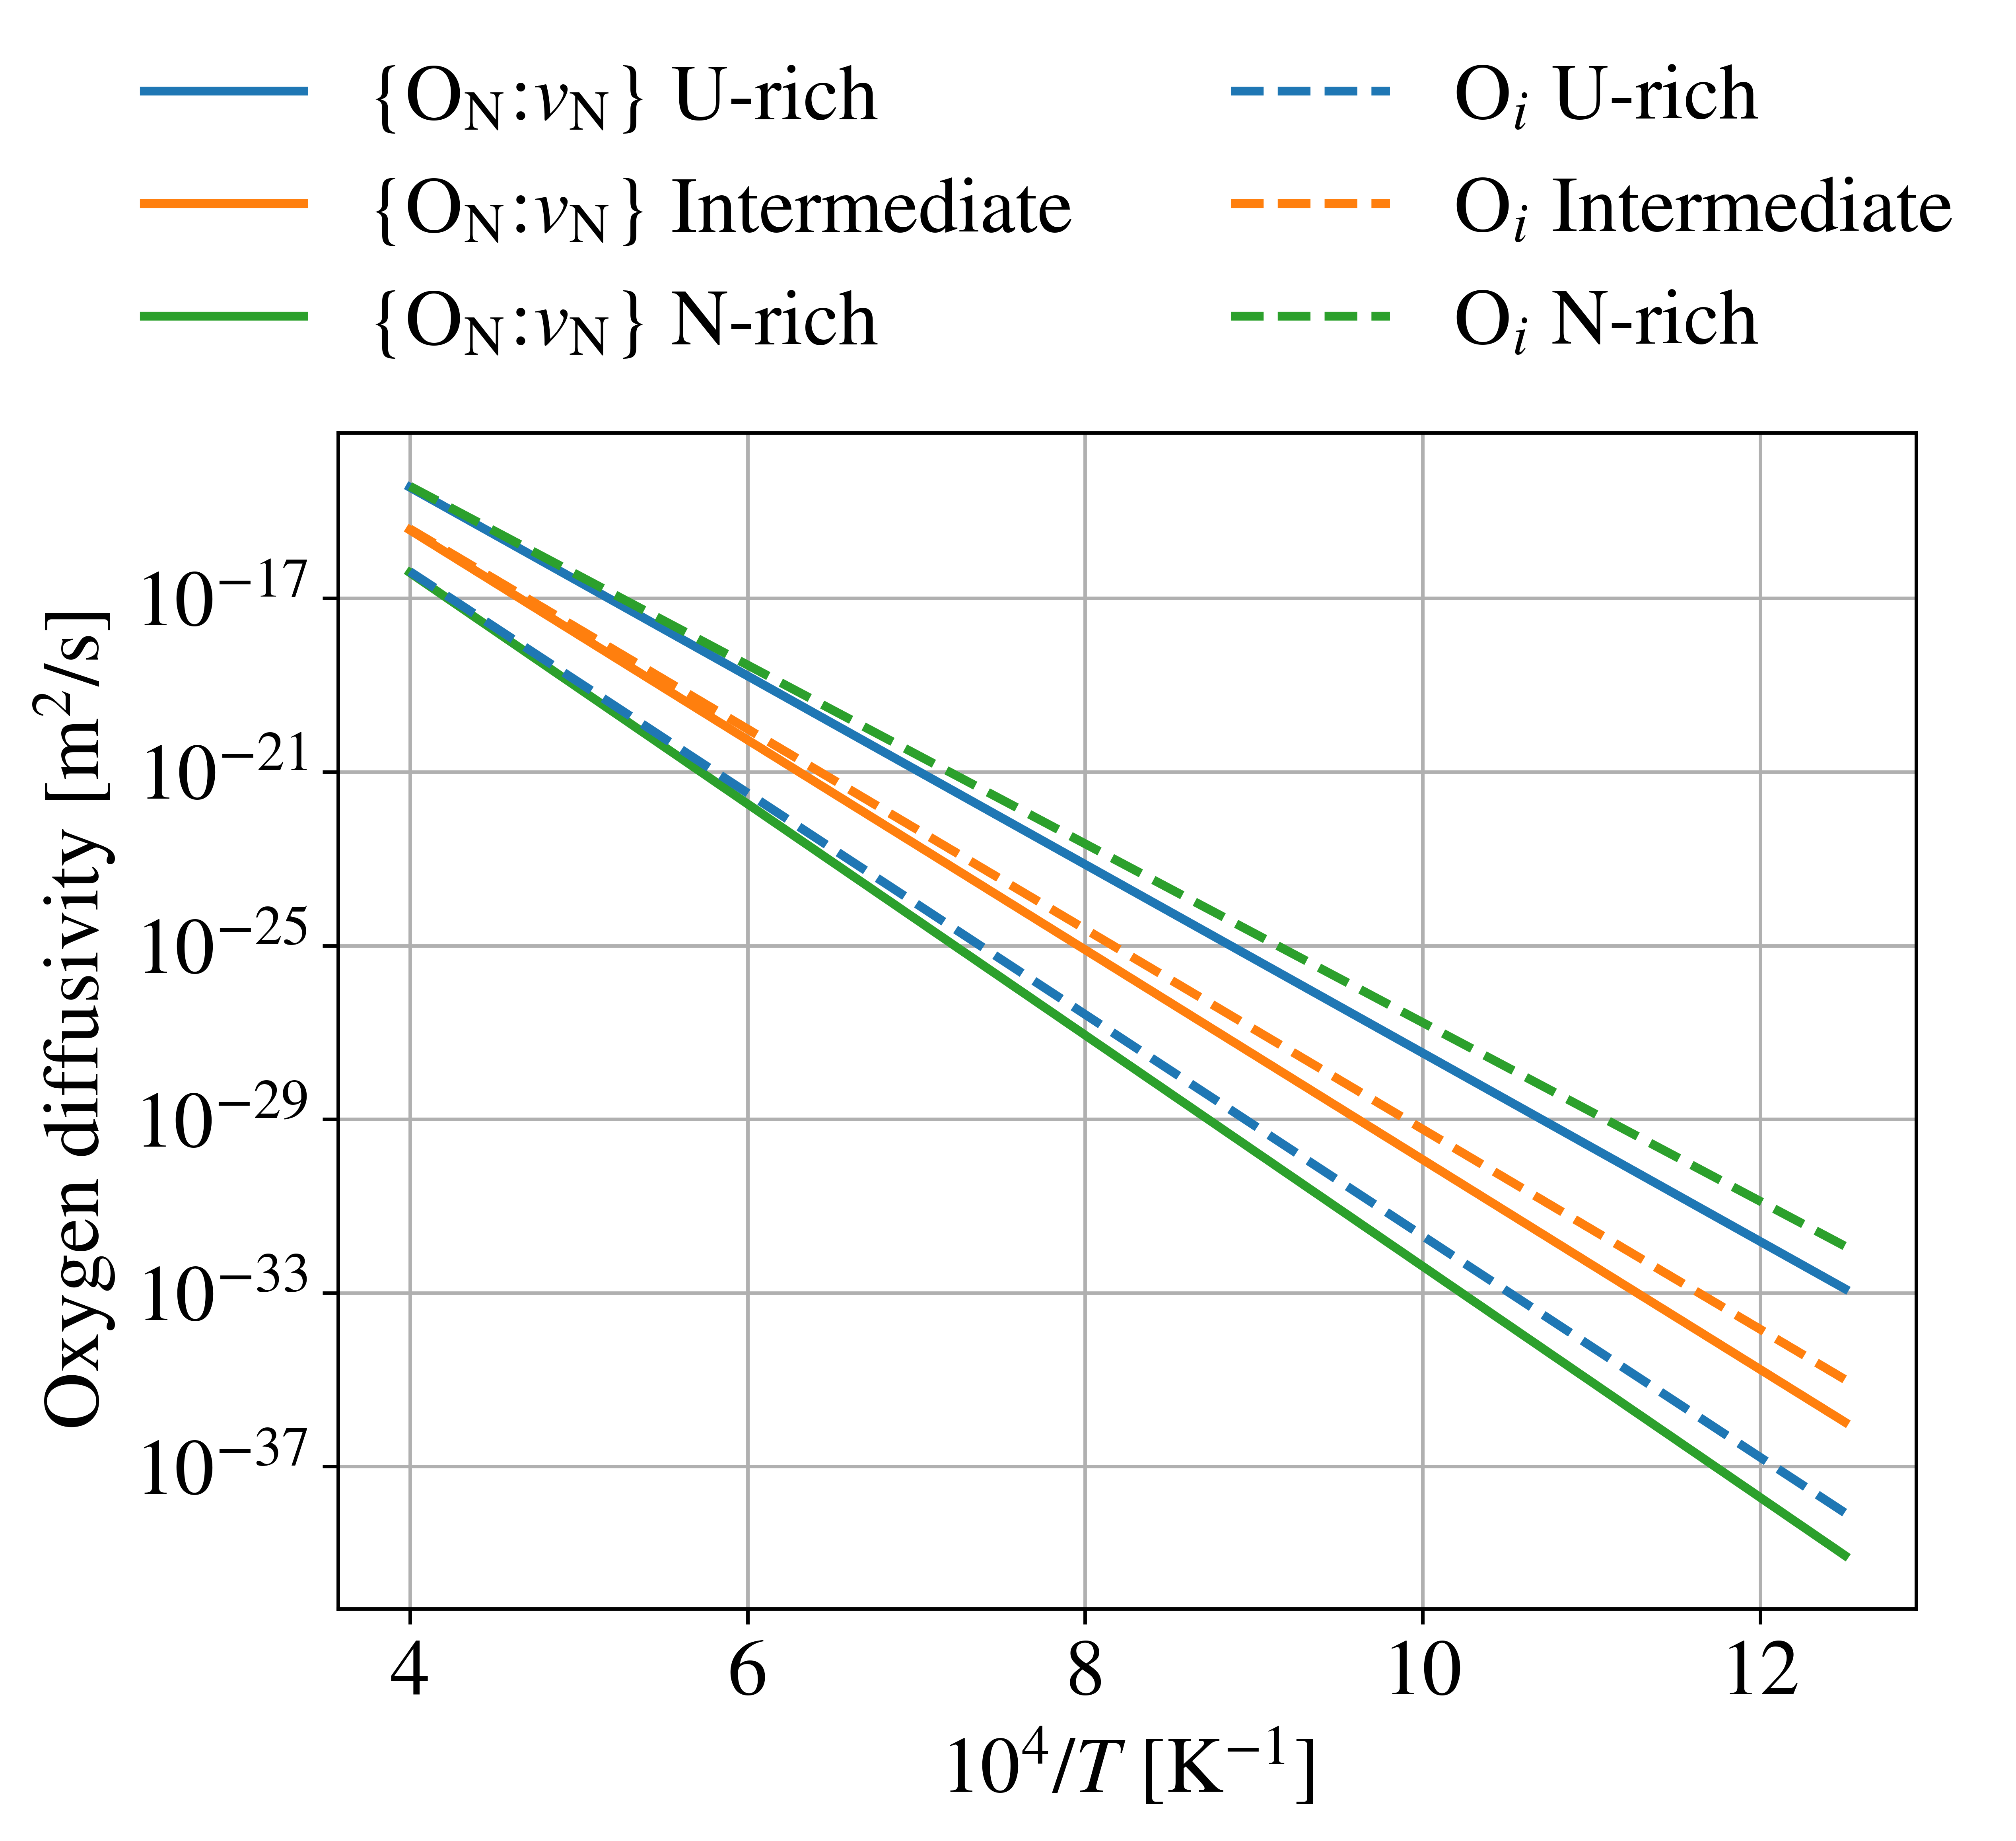
\includegraphics[width=0.5\textwidth]{DO.png}
    \caption{(Color online) Diffusivity of oxygen impurities in bulk UN by the defects $ \{\text{O}_\text{N} \! : \! v_\text{N}\} $ and $ \text{O}_i $ under U-rich (blue), Intermediate (orange), and N-rich (green) conditions.}
    \label{Fig:DO}
\end{figure}

The variation in surface energy due to oxygen adsorption and vacancy formation on void surfaces is depicted in \cref{Fig:Delta_sigma} for various porosities, oxygen concentrations, and average void radii. At low temperatures, the change in surface energy is negligible. This is because oxygen diffusivity, incorporated in the model via the kinetic correction, $\alpha_i$, is very slow at low temperatures. Within the void nucleation time, the mobility of oxygen impurities is insufficient for them to reach the void surfaces. For the reference case of $w_\text{O}$ = 1500 ppm, $p$ = 5\%, $R_v$ = 1 nm (\cref{Fig:1500_0.05_1}), the surface energy change is most significant at intermediate temperatures, around 1500 K, where breakaway swelling in UN is predicted to start \cite{Rizk2025}.

The oxygen effect on stabilizing voids is more significant at intermediate temperatures due to the balance between oxygen solubility and kinetics. At very high temperatures, the increased oxygen solubility in the bulk results in a preference for oxygen to remain in the bulk rather than adsorb onto the void surfaces. The temperature that corresponds to the maximum surface energy reduction is the same for each stoichiometric condition, independent of porosity and oxygen concentration (\cref{Fig:500_0.05_1,Fig:1500_0.05_1,Fig:3000_5_1}). This stems from the fact that the kinetic factors, $\alpha_i$, have no dependence on either porosity or oxygen concentration. The kinetic factors, however, depend on the average pore radius, i.e., $\alpha_i \sim 1/\lambda_v \sim 1/R_v$. As shown in \cref{Fig:1500_0.05_1,Fig:1500_0.05_10}, increasing $R_v$ from 1 nm to 10 nm shifts the temperature of maximum surface energy reduction by about 200 K to the right, and slightly decreases the overall magnitude of $\Delta \sigma$. This indicates that larger voids require higher temperatures for oxygen adsorption to meaningfully lower their surface energy. Nevertheless, even at elevated temperatures, the reduction in surface energy for larger voids remains smaller than that for smaller voids at the same porosity and oxygen concentration. Thus, oxygen-induced surface stabilization is most effective for small cavities, i.e., during the early stages of void nucleation and bubble growth.

% \begin{figure}[h!]
%     \centering
%     \includegraphics[width=0.5\textwidth]{Delta_sigma.png}
%     \caption{Temperature evolution of surface energy change due to oxygen adsorption and vacancy formation for oxygen weight concentration of $w_\text{O}$ = 1500 ppm, porosity of $p$ = 5\%, and average void radius of $R_v$ = 1 nm.}
%     \label{Fig:Delta_sigma}
% \end{figure}

\begin{figure}[h!]
\centering
\begin{subfigure}{0.48\textwidth}
    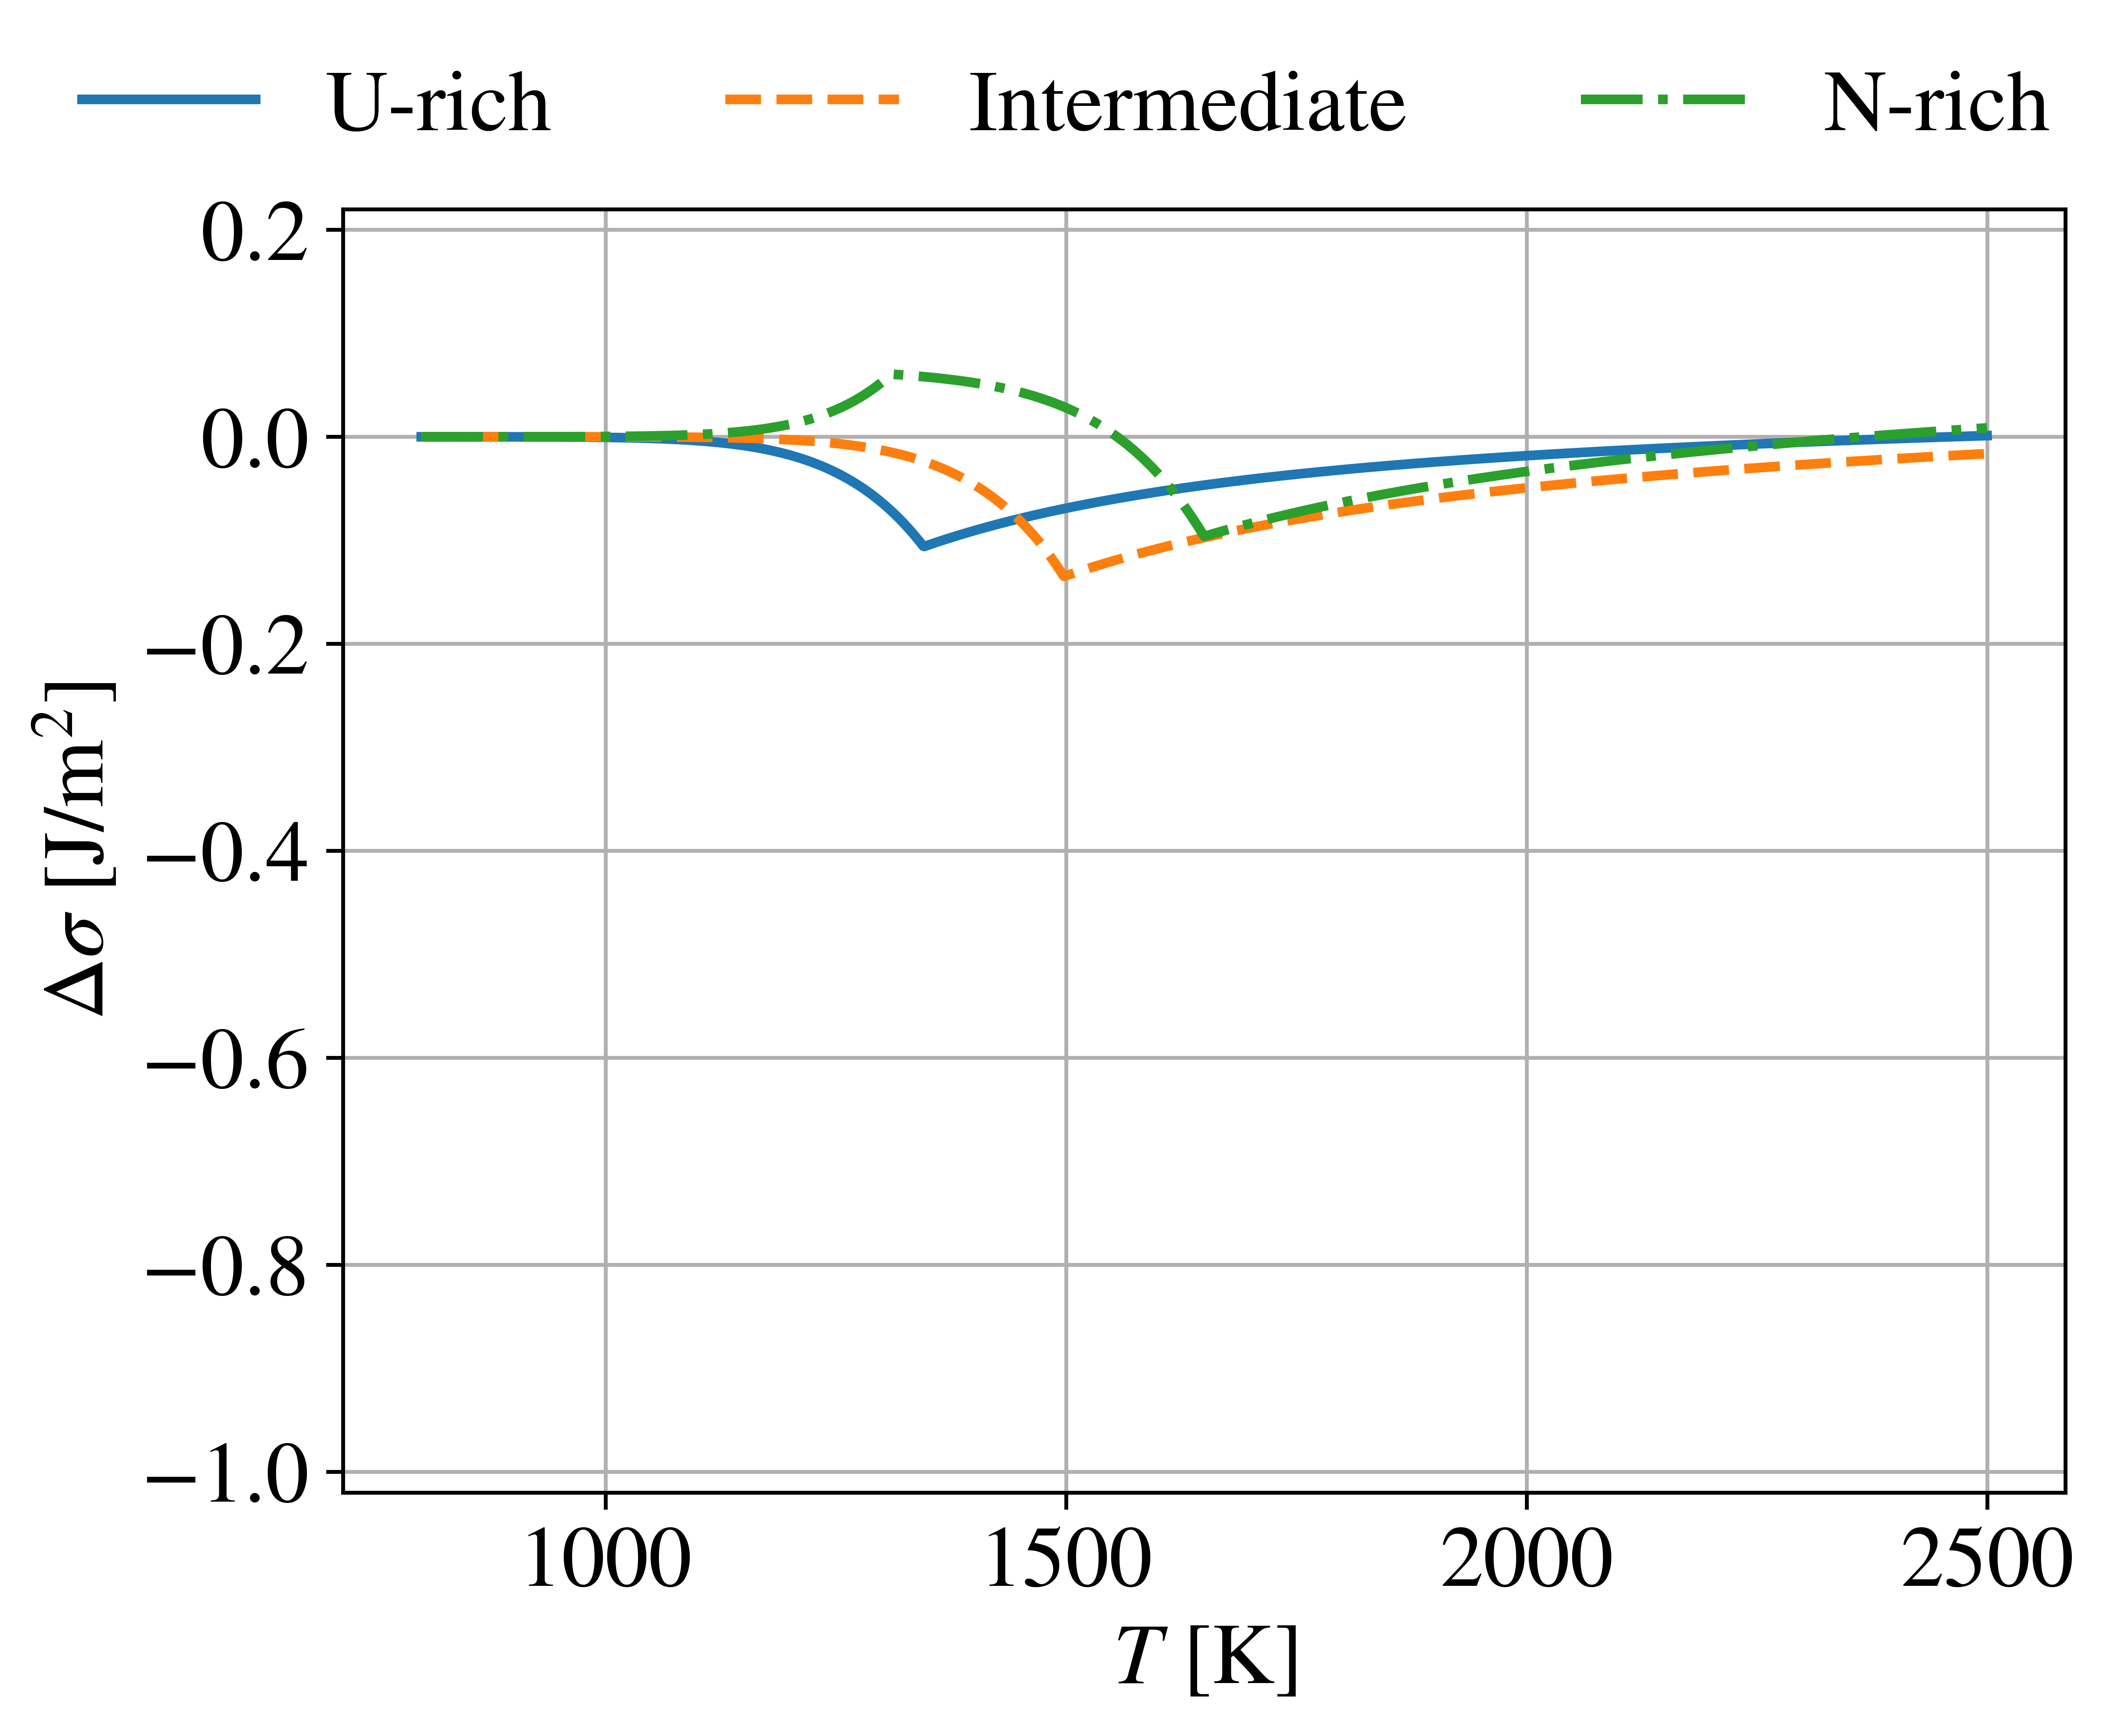
\includegraphics[width=\textwidth]{Delta_sigma_5_500_1e-09.png}
    \caption{$w_\text{O}$ = 500 ppm, $p$ = 5\%, $R_v$ = 1 nm}
    \label{Fig:500_0.05_1}
\end{subfigure}
\hfill
\begin{subfigure}{0.48\textwidth}
    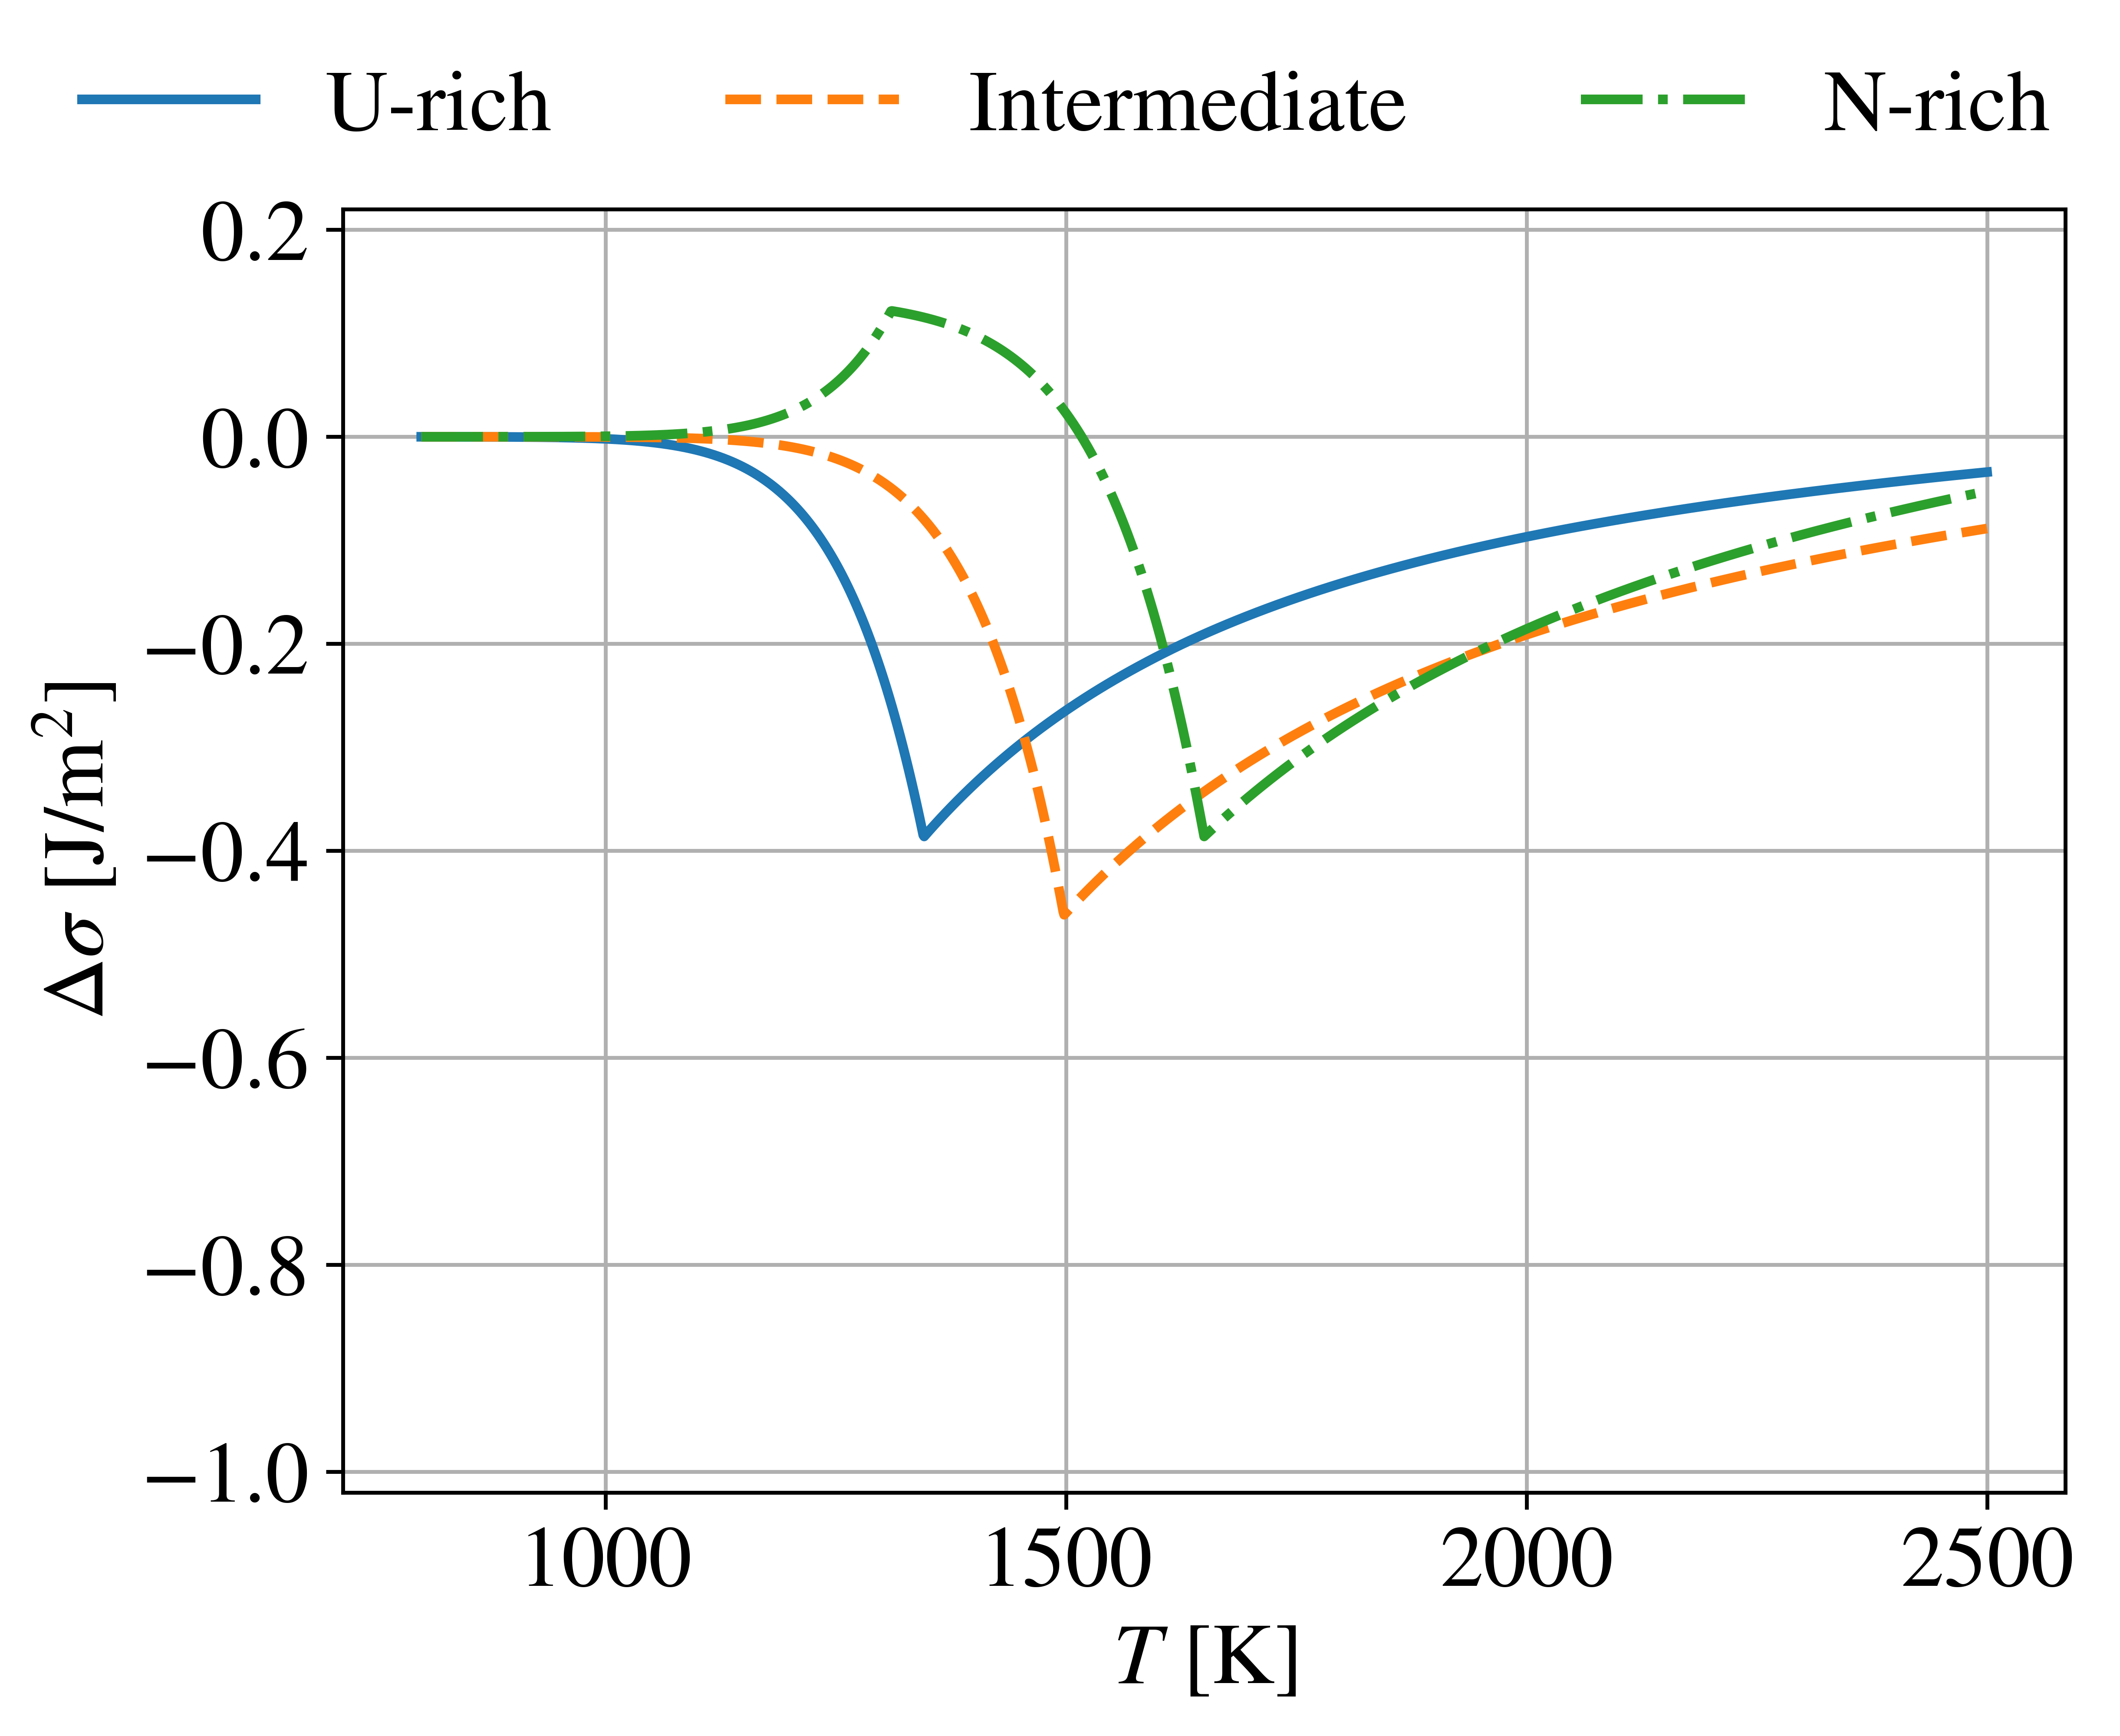
\includegraphics[width=\textwidth]{Delta_sigma_5_1500_1e-09.png}
    \caption{$w_\text{O}$ = 1500 ppm, $p$ = 5\%, $R_v$ = 1 nm}
    \label{Fig:1500_0.05_1}
\end{subfigure}
\hfill
\begin{subfigure}{0.48\textwidth}
    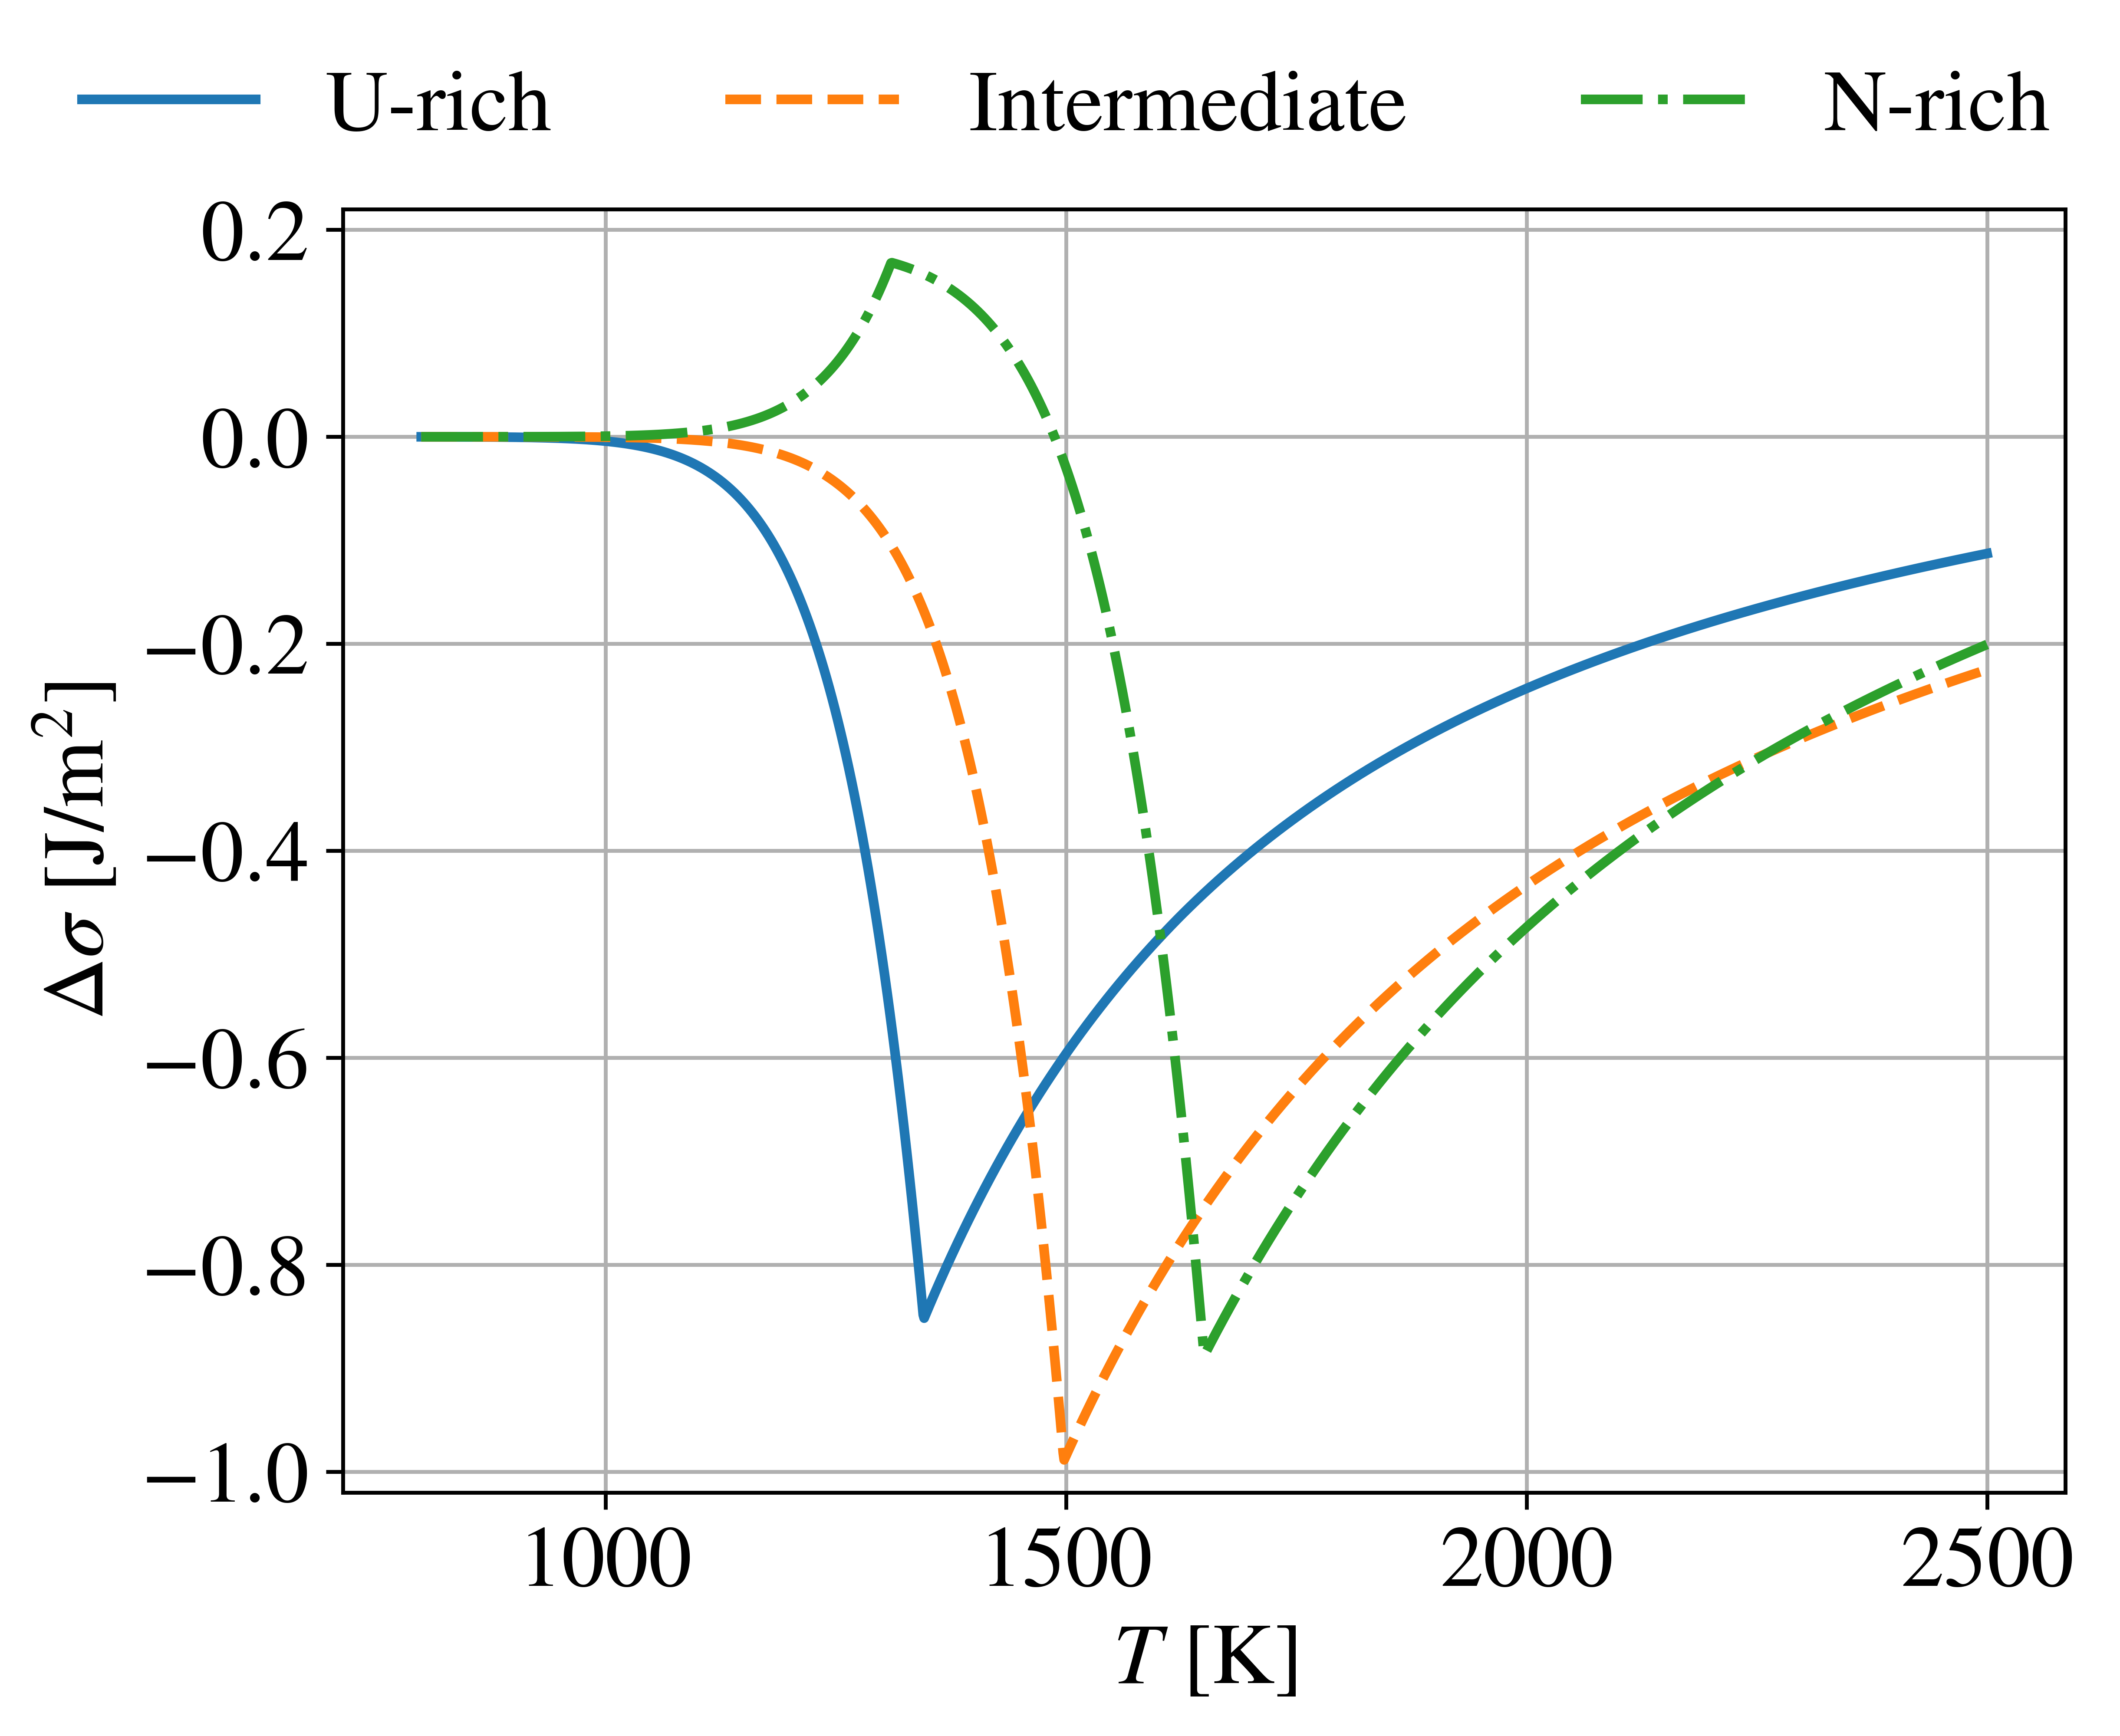
\includegraphics[width=\textwidth]{Delta_sigma_5_3000_1e-09.png}
    \caption{$w_\text{O}$ = 3000 ppm, $p$ = 5\%, $R_v$ = 1 nm}
    \label{Fig:3000_5_1}
\end{subfigure}
\begin{subfigure}{0.48\textwidth}
    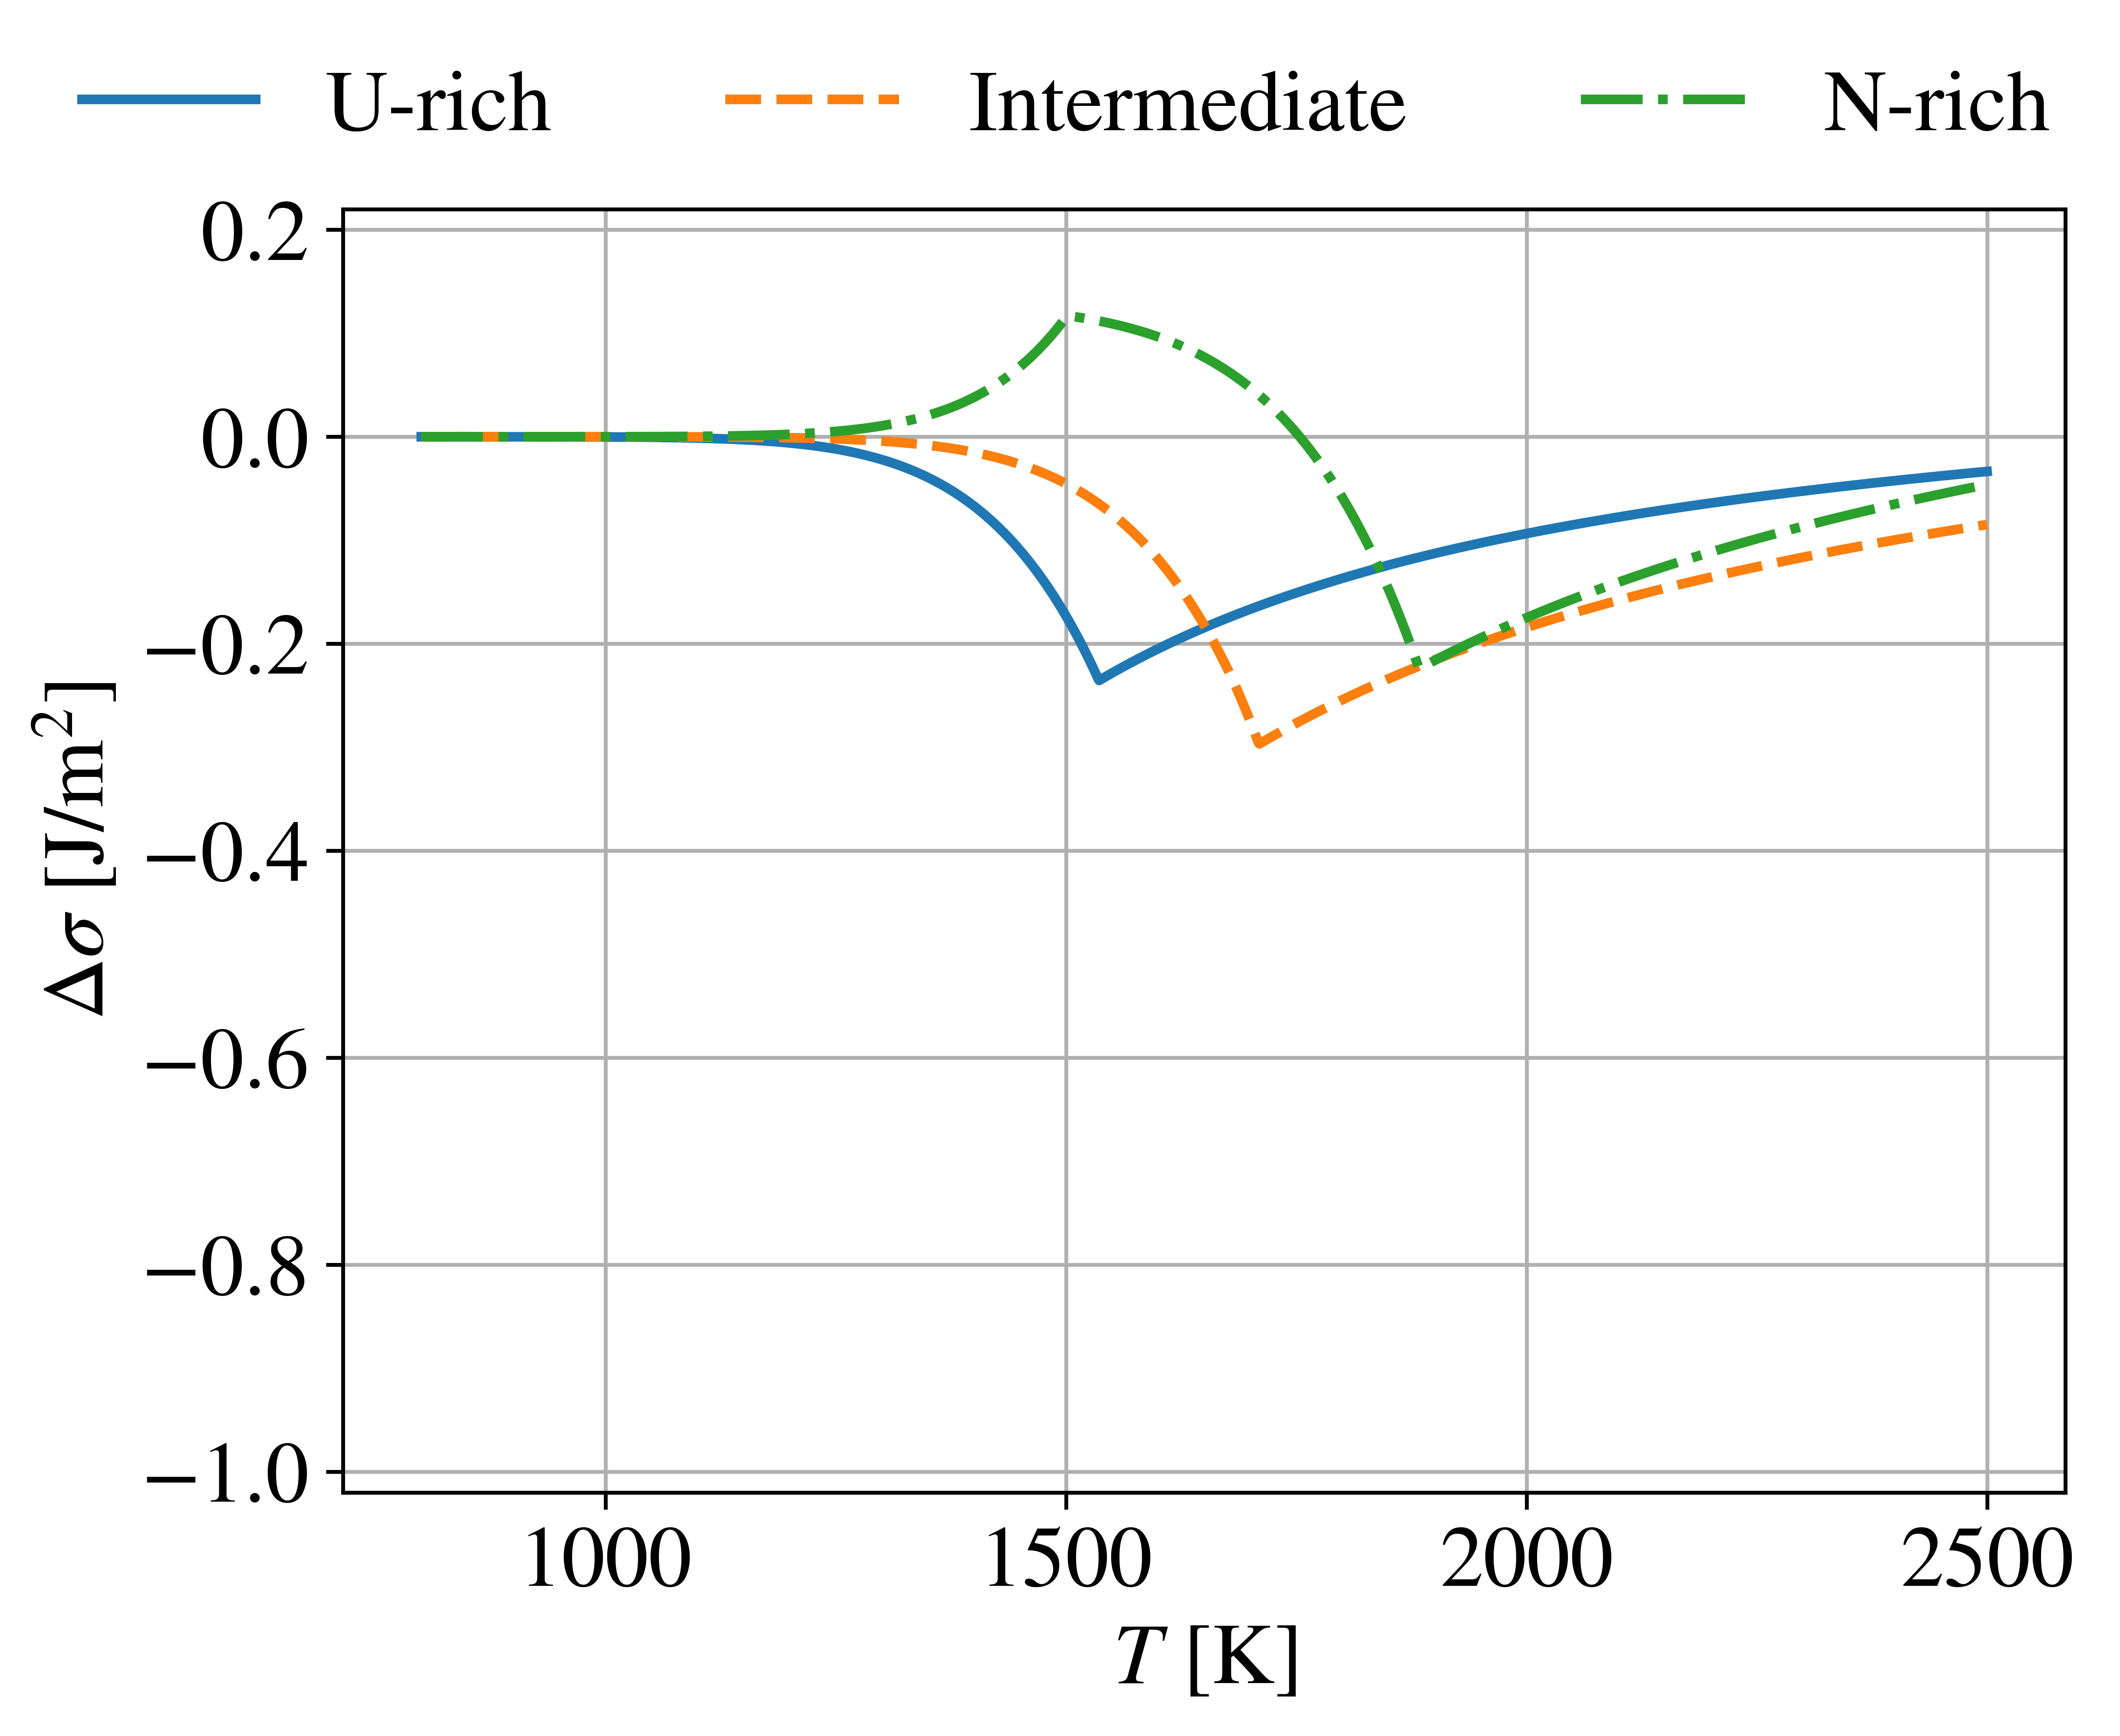
\includegraphics[width=\textwidth]{Delta_sigma_5_1500_1e-08.png}
    \caption{$w_\text{O}$ = 1500 ppm, $p$ = 5\%, $R_v$ = 10 nm}
    \label{Fig:1500_0.05_10}
\end{subfigure}
% \hfill
% \begin{subfigure}{0.3\textwidth}
%     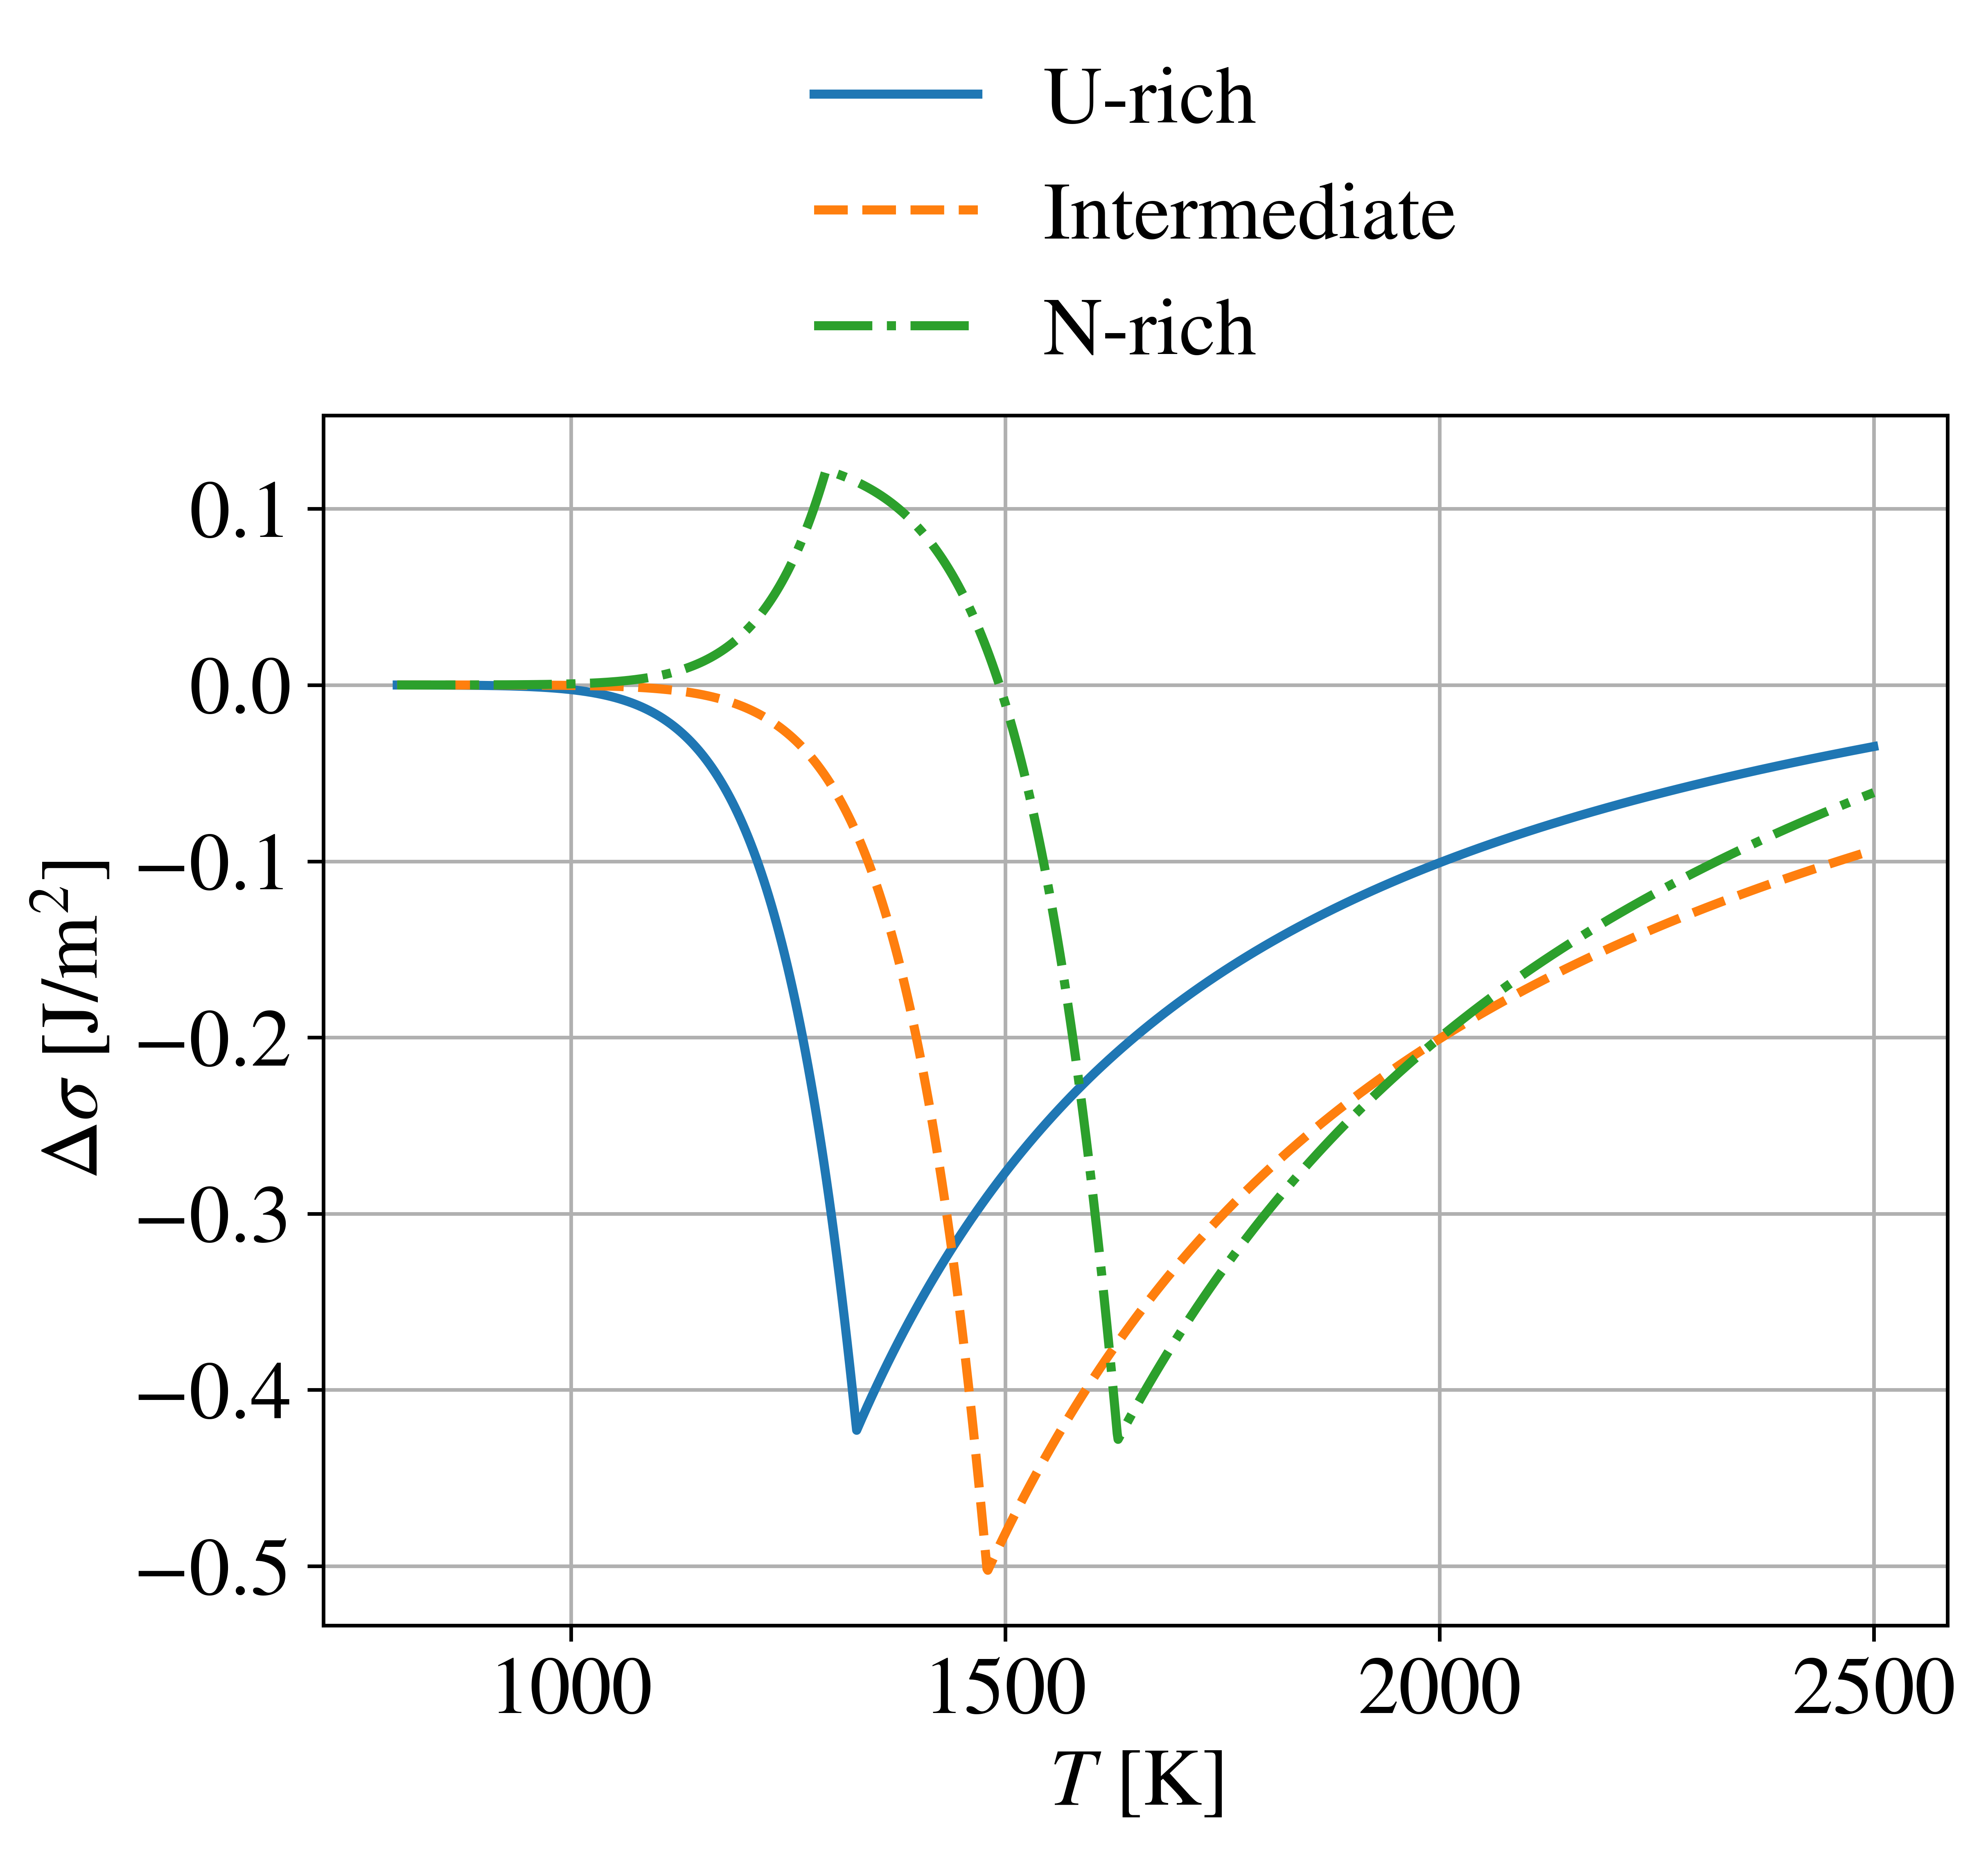
\includegraphics[width=\textwidth]{Delta_sigma_0.1_1500.0_1e-09.png}
%     \caption{$w_\text{O}$ = 1500 ppm, $p$ = 10\%, $R_v$ = 1 nm}
%     \label{Fig:1500_0.10_1}
% \end{subfigure}
% \hfill
% \begin{subfigure}{0.3\textwidth}
%     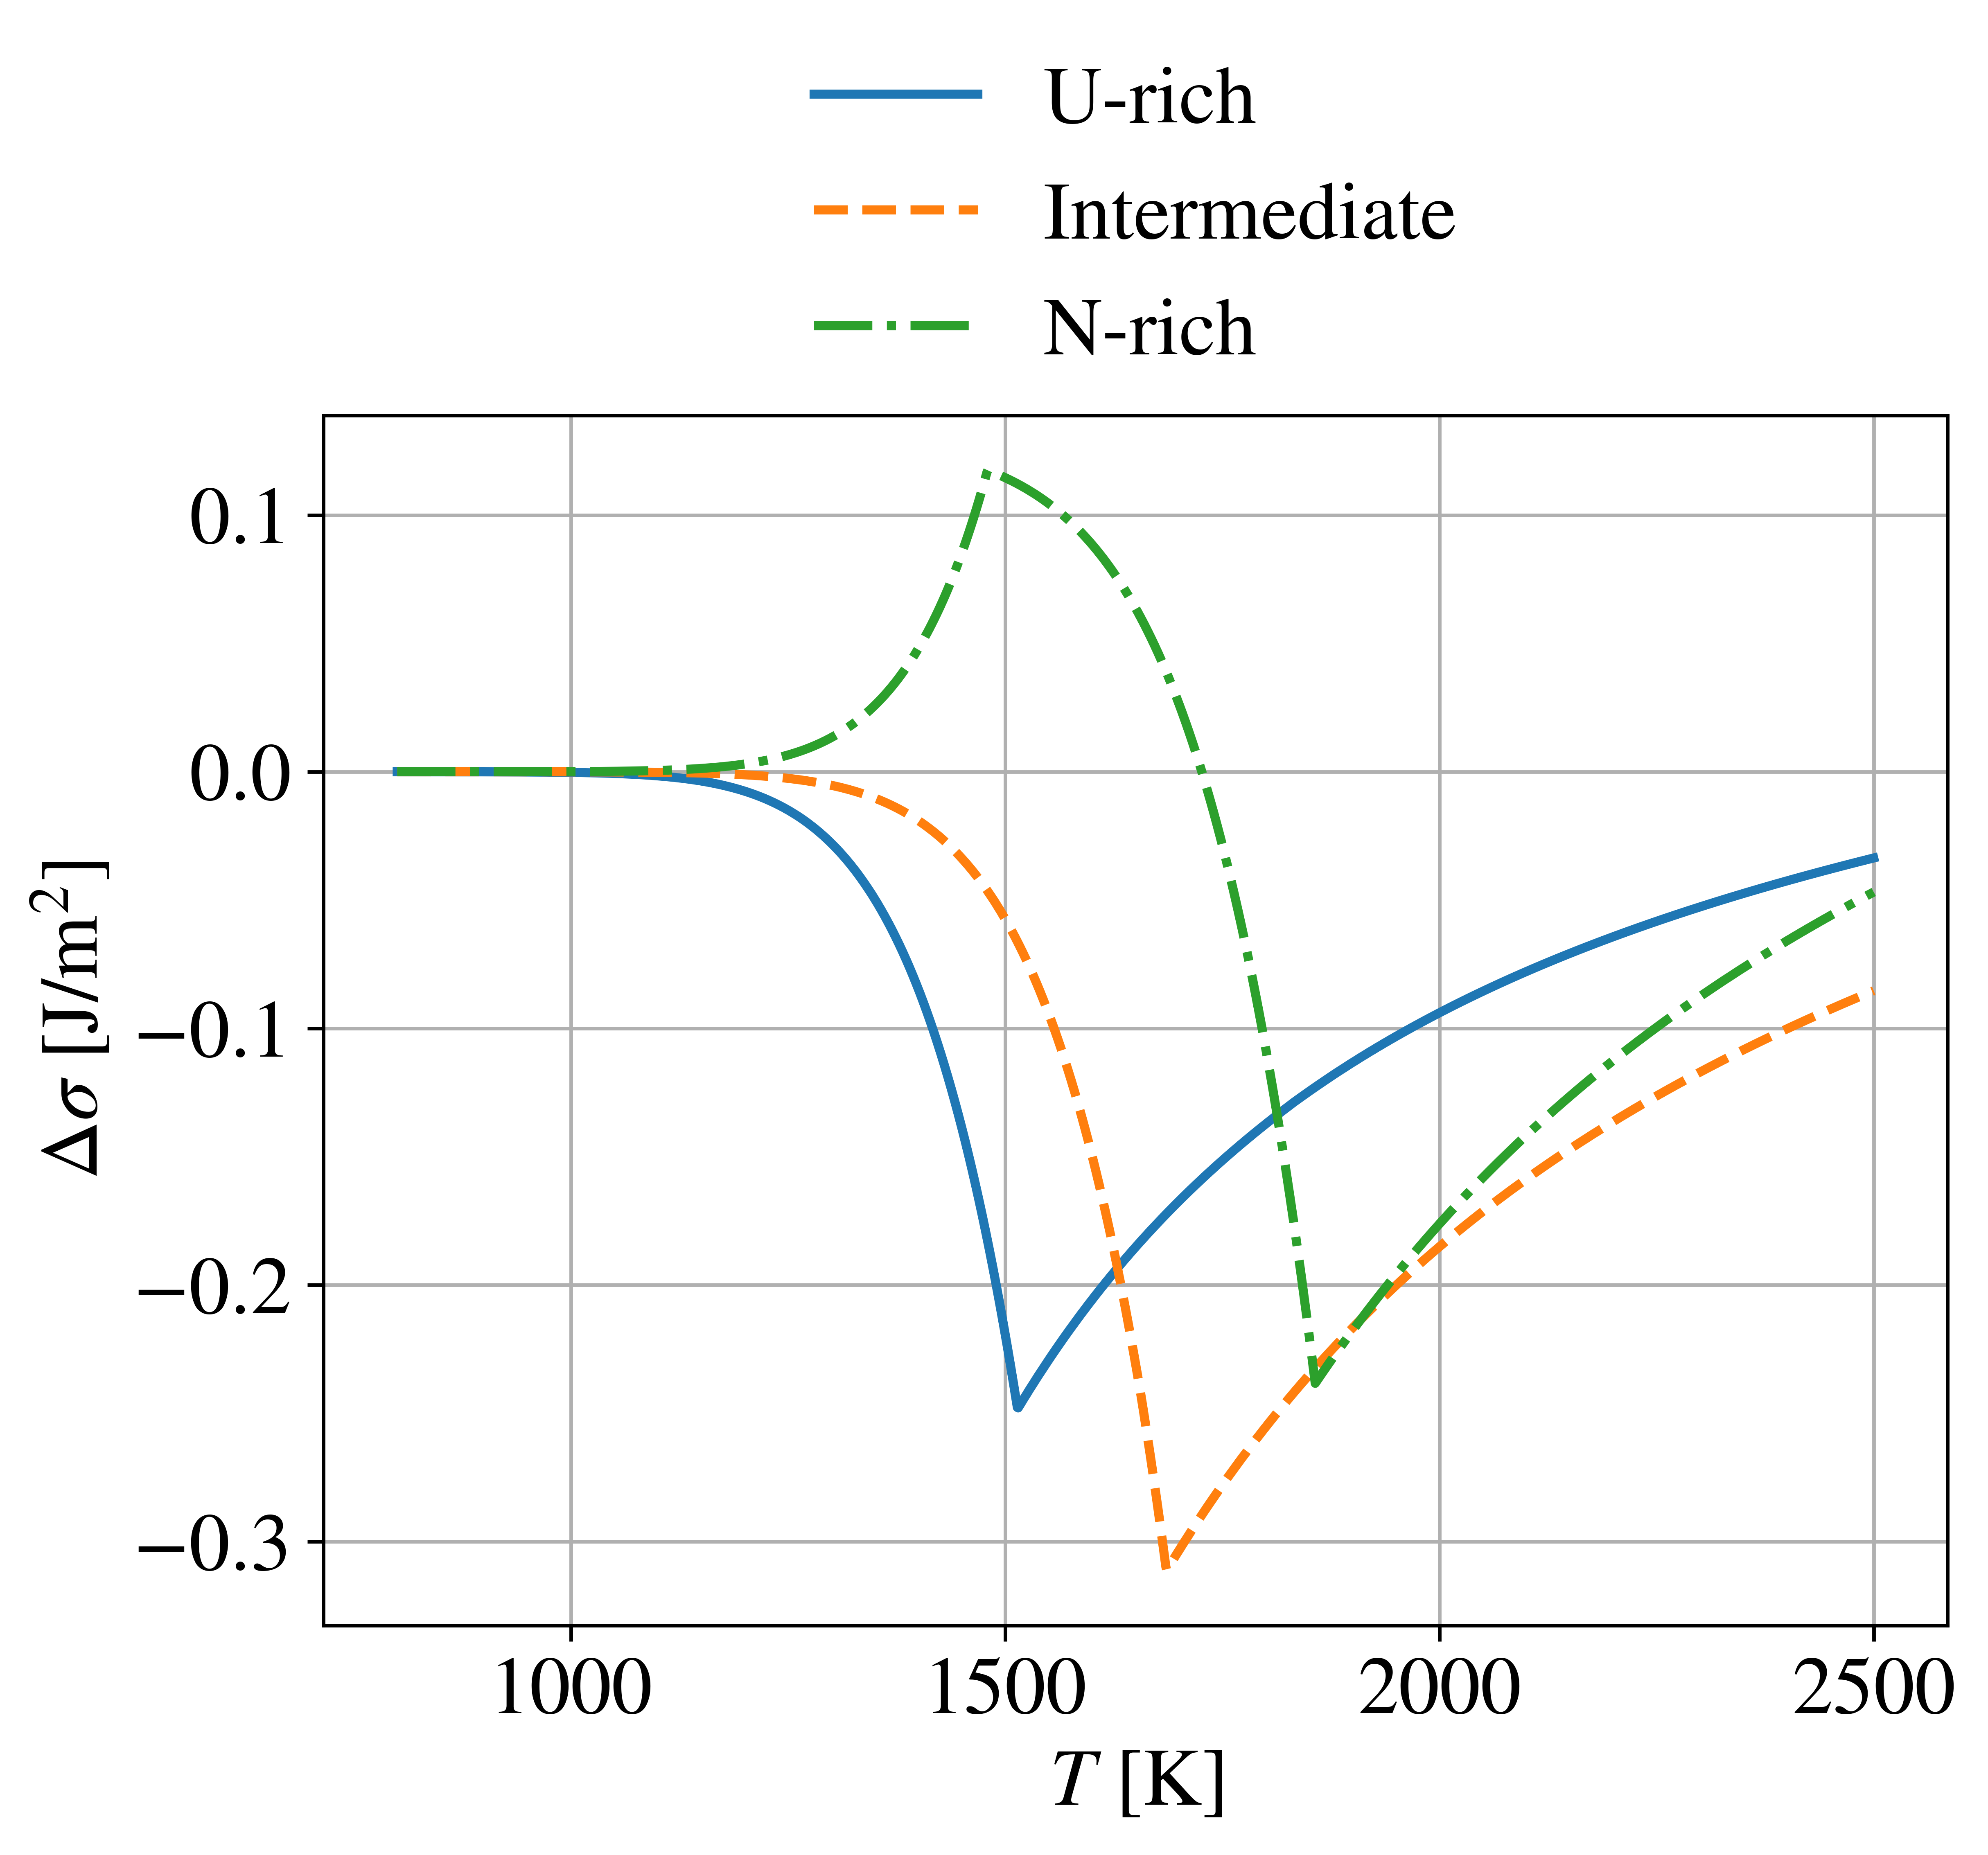
\includegraphics[width=\textwidth]{Delta_sigma_0.1_1500.0_1e-08.png}
%     \caption{$w_\text{O}$ = 1500 ppm, $p$ = 10\%, $R_v$ = 10 nm}
%     \label{Fig:1500_0.10_10}
% \end{subfigure}
\caption{Temperature evolution of surface energy change due to oxygen adsorption and vacancy formation for various porosities, oxygen concentrations, and average void radii.}
\label{Fig:Delta_sigma}
\end{figure}

It is of interest to examine the contribution of the different terms to the change in surface energy, where $\Delta \sigma ( \text{O}_\text{N}^\text{(s)} )$ (\cref{Eq:D1}) represents the contribution of $\text{O}_\text{N}^\text{(s)}$ to $\Delta \sigma$, with analogous definitions for $\Delta \sigma ( \text{O}_i^\text{(s)} )$ (\cref{Eq:D2}) and $\Delta \sigma ( v_\text{N}^\text{(s)} )$ (\cref{Eq:D3}). 

\begin{equation}
\Delta \sigma ( \text{O}_\text{N}^{\text{(s)}} ) = \frac{8}{3} \frac{1-p}{p} \frac{R_v}{a^3} c_\text{O} \alpha_1 \frac{ [ \text{O}_\text{N}^{\text{(s)}} ] }{ [ \text{O}_\text{N}^{\text{(b)}} ] }  E_\text{ad}( \text{O}_\text{N}^{\text{(s)}} ).
\label{Eq:D1}
\end{equation}

\begin{equation}
\Delta \sigma ( \text{O}_i^{\text{(s)}} ) = \frac{8}{3} \frac{1-p}{p} \frac{R_v}{a^3} c_\text{O} \alpha_2 \frac{ [ \text{O}_i^{\text{(s)}} ] }{ [ \text{O}_\text{N}^{\text{(b)}} ] }  E_\text{ad}( \text{O}_i^{\text{(s)}} ).
\label{Eq:D2}
\end{equation}

\begin{equation}
\Delta \sigma (v_\text{N}^{\text{(s)}}) = \frac{2}{a^2} [ v_\text{N}^{\text{(s)}} ] E_f ( v_\text{N}^{\text{(s)}} ).
\label{Eq:D3}
\end{equation}

\noindent These terms are plotted in \cref{Fig:D}. Comparing \cref{Fig:Delta_sigma,Fig:D1}, it can be seen that the adsorption of oxygen as $\text{O}_\text{N}^\text{(s)}$ dominates the $\Delta \sigma$ profile. This is expected since $\text{O}_\text{N}^\text{(s)}$ is the most dominant oxygen adsorption site (refer to \cref{Fig:Ois_ONs}) and it leads to a reduction of surface energy at all temperatures (also see \cref{Fig:EadONs}). From \cref{Fig:D2}, it can be observed that $\text{O}_i^\text{(s)}$ is responsible for the slight surface energy increase in the range of 1020--1520 K in the N-rich profile of \cref{Fig:Delta_sigma}. Finally, in \cref{Fig:D3}, it is obvious that the formation of N vacancies has a negligible contribution to the surface energy change of voids.

\begin{figure}[h!]
\centering
\begin{subfigure}{0.48\textwidth}
    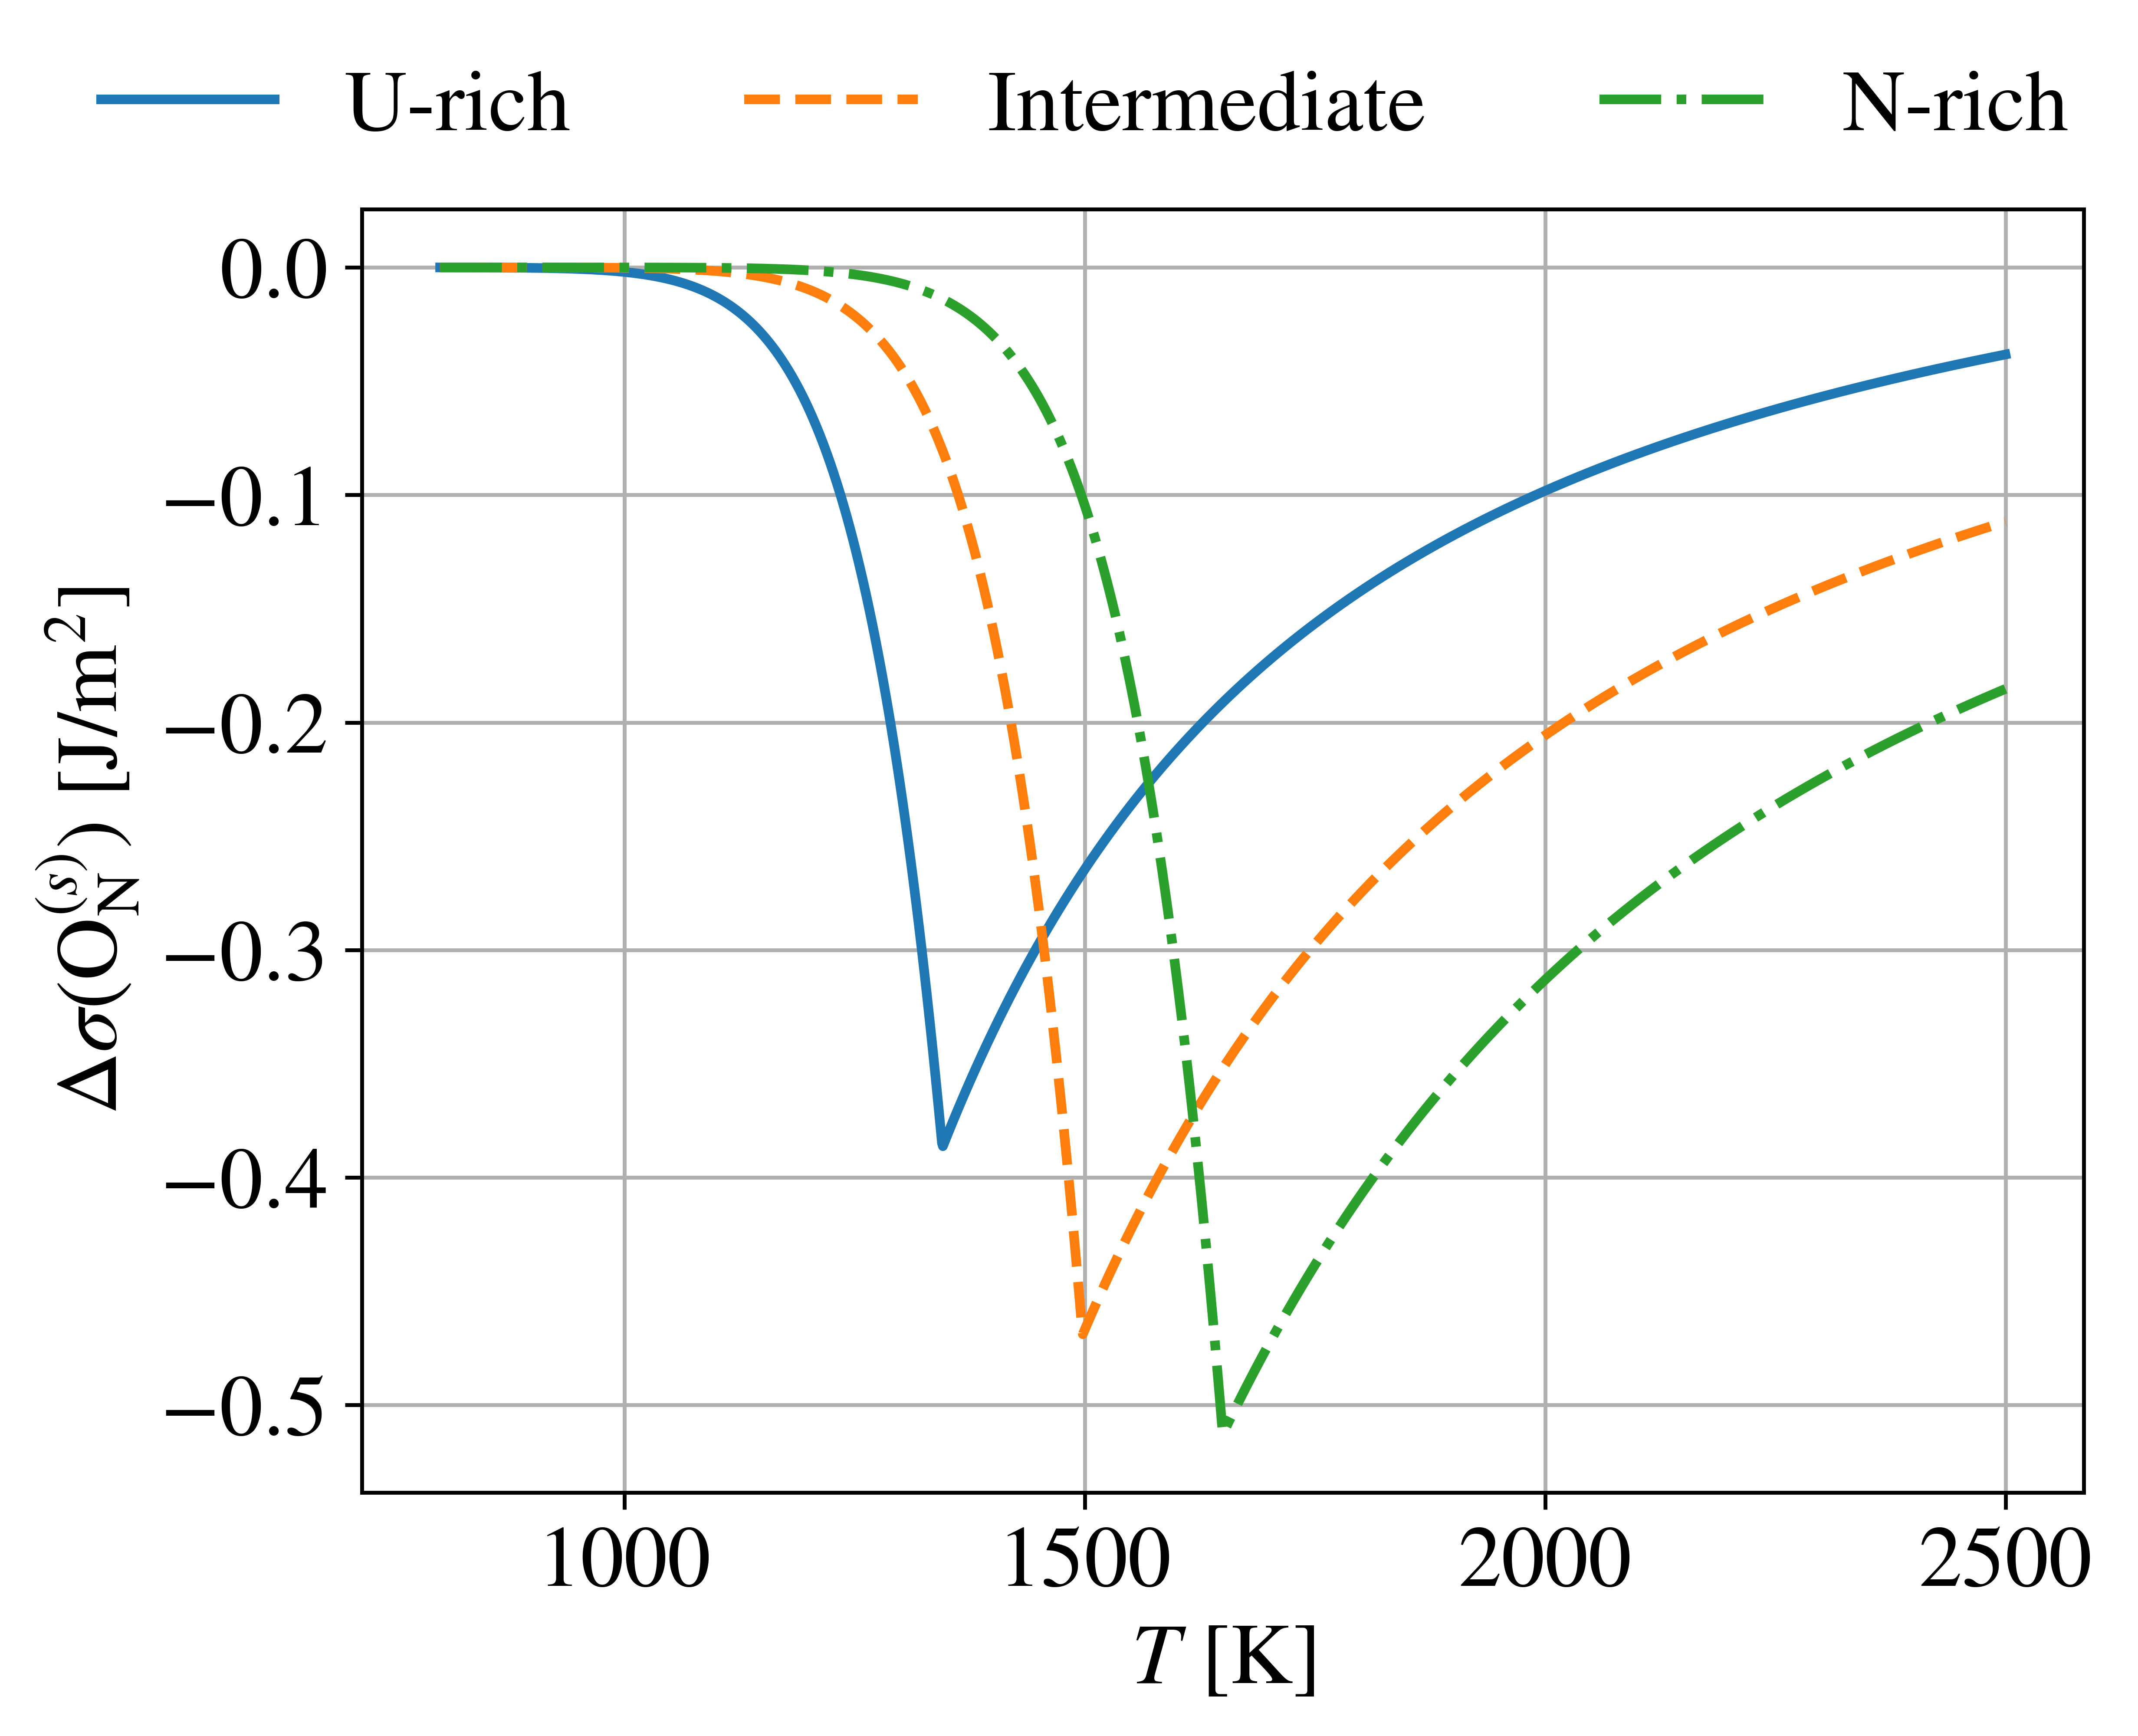
\includegraphics[width=\textwidth]{Delta1.png}
    \caption{}
    \label{Fig:D1}
\end{subfigure}
\hfill
\begin{subfigure}{0.48\textwidth}
    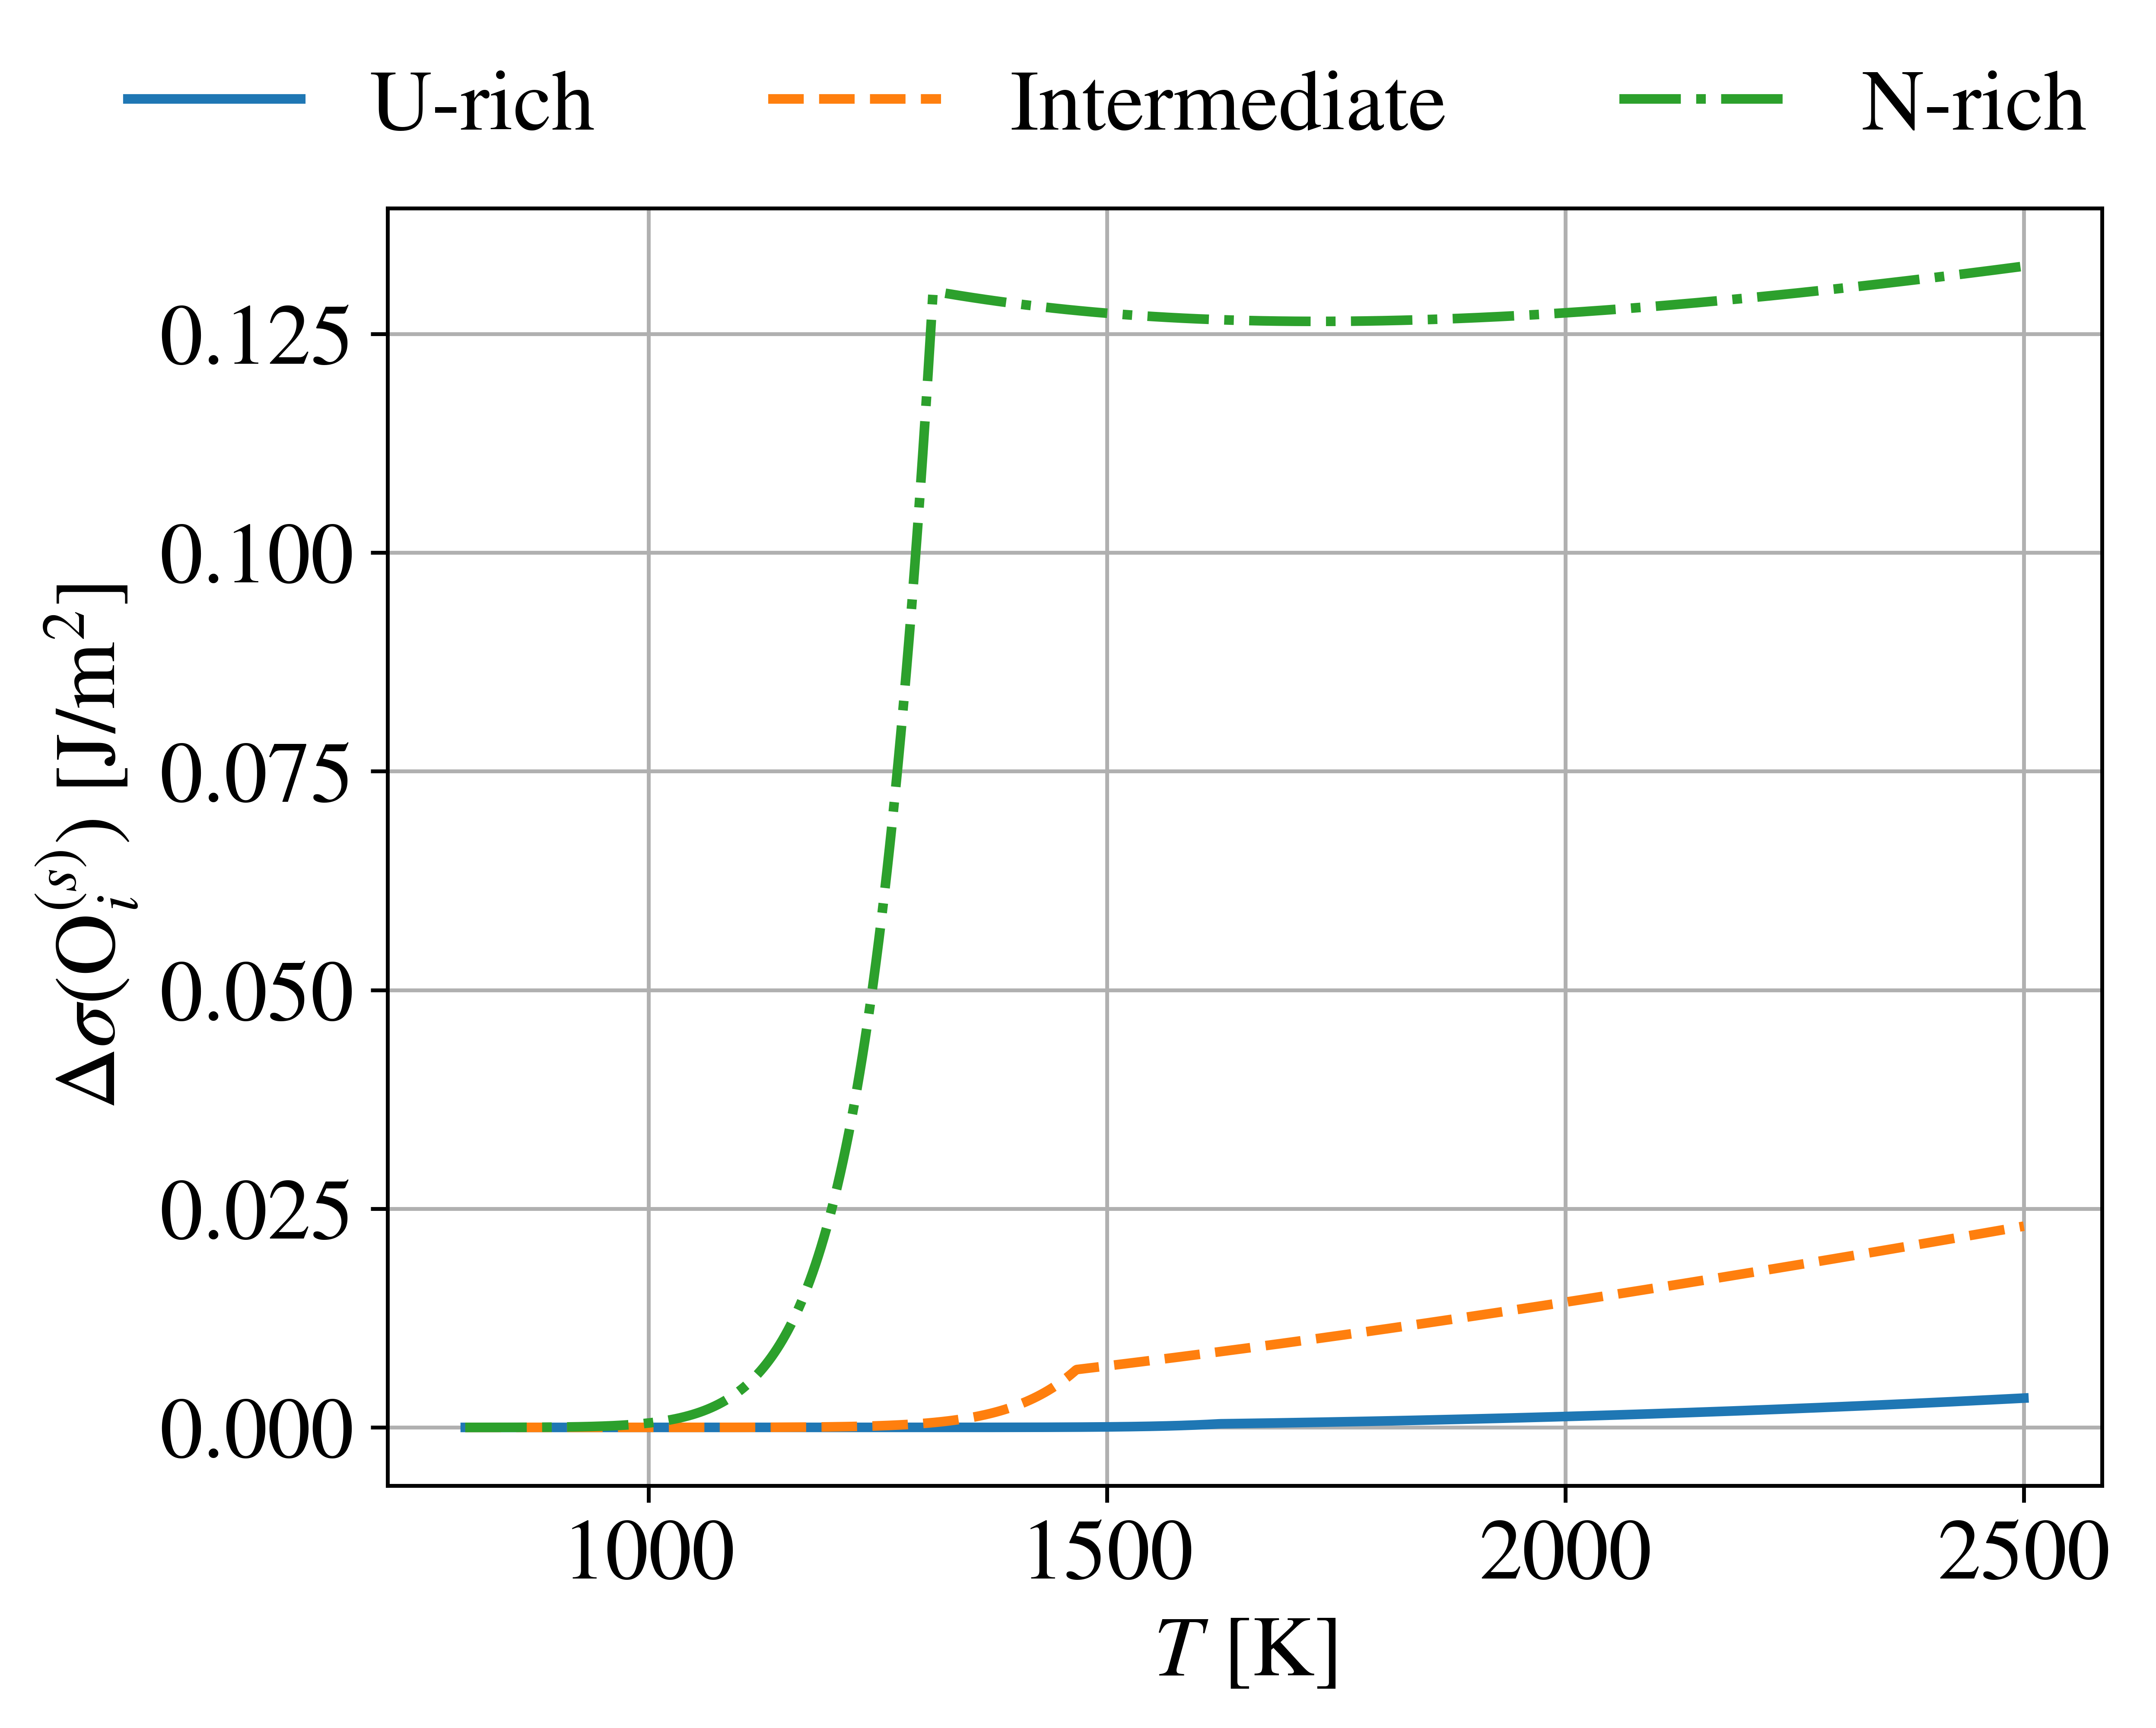
\includegraphics[width=\textwidth]{Delta2.png}
    \caption{}
    \label{Fig:D2}
\end{subfigure}
\hfill
\begin{subfigure}{0.48\textwidth}
    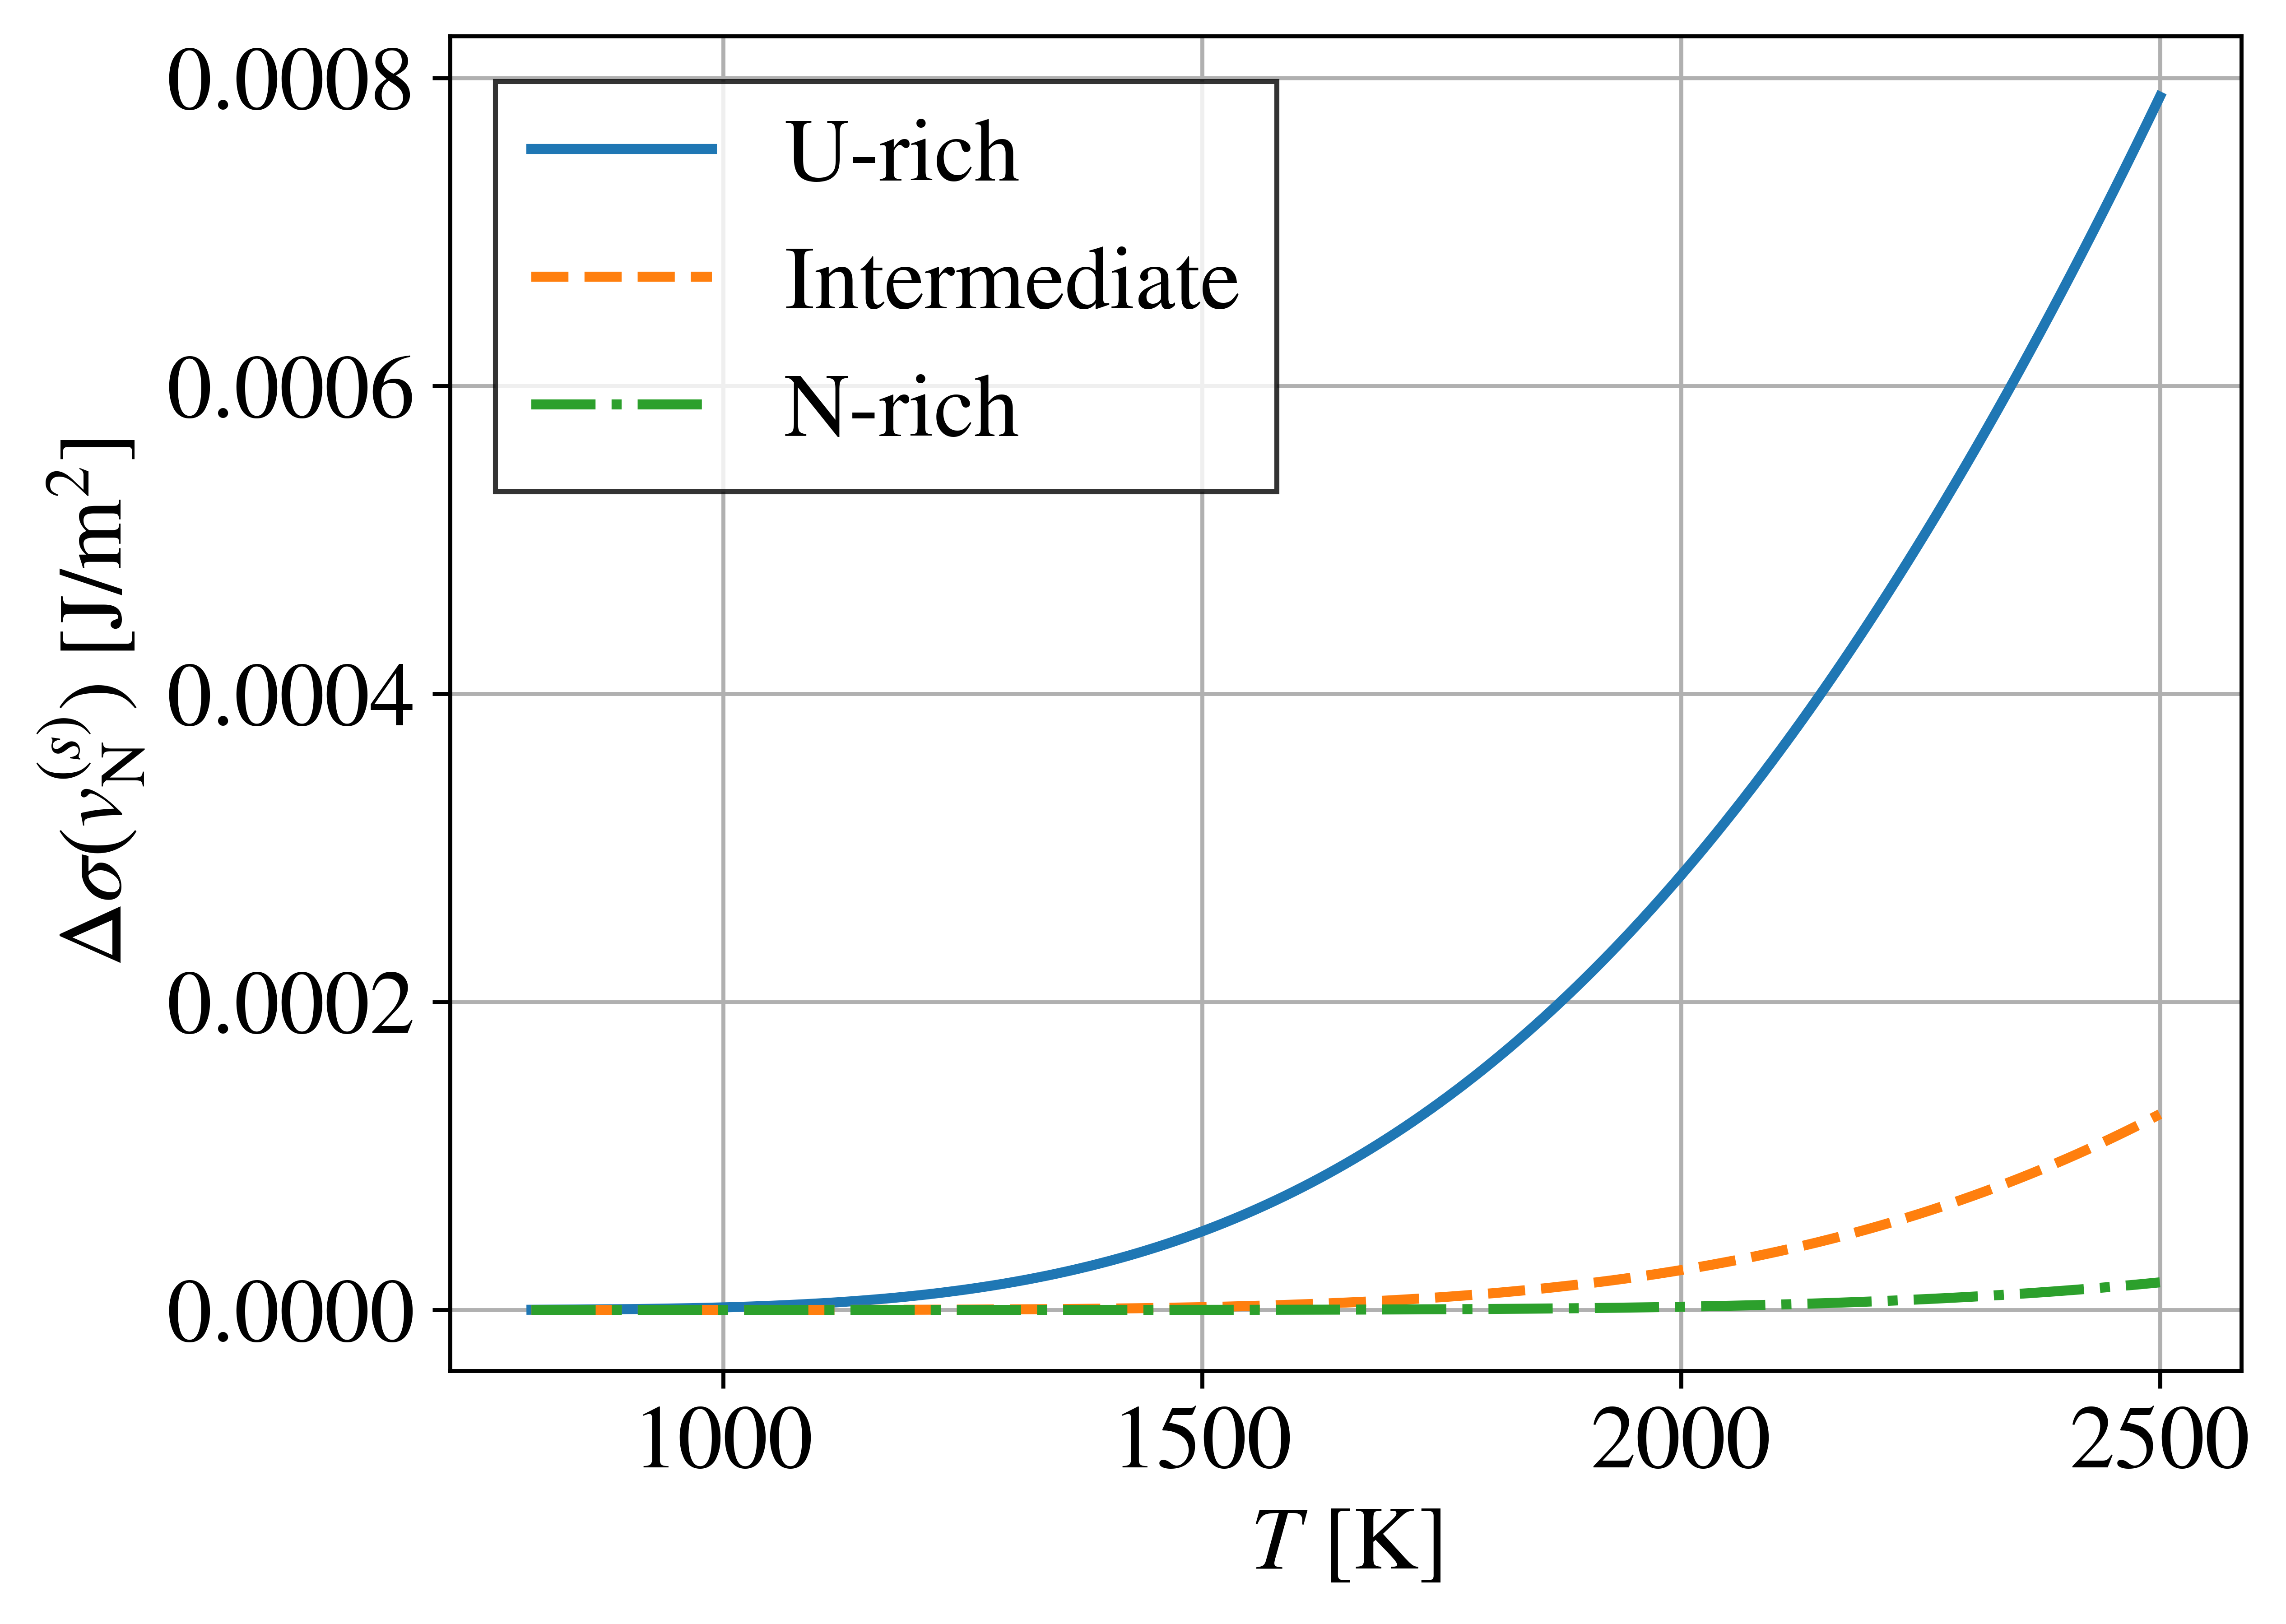
\includegraphics[width=\textwidth]{Delta3.png}
    \caption{}
    \label{Fig:D3}
\end{subfigure}
\caption{Different terms of the surface energy change due to oxygen adsorption and vacancy formation on void surfaces for $w_\text{O}$ = 1500 ppm, $p$ = 5\%, and $R_v$ = 1 nm. \textbf{(a)} $\Delta \sigma ( \text{O}_\text{N}^{\text{(s)}} )$, \textbf{(b)} $\Delta \sigma ( \text{O}_i^{\text{(s)}} )$, and \textbf{(c)} $\Delta \sigma (v_\text{N}^{\text{(s)}})$ are given in \cref{Eq:D1,Eq:D2,Eq:D3}, respectively.}
\label{Fig:D}
\end{figure}

Given that the effect of nitrogen vacancies on surface energy reduction is negligible, and the contribution of $\text{O}_i^{\text{(s)}}$ is second order, the $\Delta \sigma$ formula (\cref{Eq:DeltaSigma1}) simplifies to a product of four terms: a geometric factor $\eta = ((1 - p)/p) \cdot R_v/3$, the oxygen number density $n_\text{O} = c_\text{O} / \Omega$, a kinetic correction factor $\alpha_1$, and an effective segregation energy $E_\text{seg}^\text{eff} = ( [\text{O}_\text{N}^{(\text{s})}] / [\text{O}_\text{N}^{(\text{b})}] ) \, E_\text{ad}(\text{O}_\text{N}^{(\text{s})})$. Specifically, we write:
\begin{equation}
\Delta \sigma \approx \left( \frac{(1 - p)}{p} \, \frac{R_v}{3} \right) \cdot \frac{c_\text{O}}{\Omega} \cdot \alpha_1 \cdot \left( \frac{ [ \text{O}_\text{N}^{(\text{s})} ] }{ [ \text{O}_\text{N}^{(\text{b})} ] } \, E_\text{ad}( \text{O}_\text{N}^{(\text{s})} ) \right) = \eta \, n_\text{O} \, \alpha_1 \, E_\text{seg}^\text{eff},
\label{Eq:DeltaSigmaSimple}
\end{equation}
where $c_\text{O}$ is the atomic fraction of oxygen, $\Omega = a^3/8$ is the atomic volume of the matrix (inverse of the atomic number density), $p$ is the porosity, and $R_v$ is the average void radius. The geometric factor $\eta$ captures the matrix-to-void volume ratio, $(1-p)/p$, and the void volume-to-surface ratio, $R_v/3$. That is, $\eta$ represents the average matrix volume per unit void surface area: $(V_\text{matrix}/V_\text{void}) \times (V_\text{void}/A_\text{void}) = V_\text{matrix} / A_\text{void}$, and gives a length scale that quantifies an effective thickness of matrix material 
supplying each unit of void surface. The kinetic correction factor $\alpha_1$ accounts for the finite diffusivity of oxygen within the void nucleation timescale (refer to \cref{Eq:alpha}). Finally, $E_\text{seg}^\text{eff}$ represents the net energy gain per oxygen atom that segregates to the void surface. This formulation makes explicit that the surface energy reduction is governed by the interplay of thermodynamics, kinetics, and microstructural geometry, and scales linearly with the number of oxygen atoms that successfully reach and adsorb on the available void surface area. Note that the temperature dependence of $|\Delta \sigma|$ is contained in the anti-Arrhenius term $[\text{O}_\text{N}^{(\text{s})}] / [\text{O}_\text{N}^{(\text{b})}]$ and $\alpha_1 \sim \sqrt{D_1}$.



For the reference case of $w_\text{O}$ = 1500 ppm, $p$ = 5\%, and $R_v$ = 1 nm, $|\Delta \sigma|$ is found to be around 0.4~J/m$^2$, occurring within the temperature interval 1300--1700~K (see \cref{Fig:1500_0.05_1}). To assess the sensitivity of $|\Delta \sigma|$ to key parameters, we vary $w_\text{O}$ and $p$ while holding $R_v$ fixed at 25 nm, which is a typical size for both dislocations and intergranular bubbles \cite{Colin1983}. It has been shown that dislocation bubbles dominate bubble swelling in UN \cite{Ronchi1975,Ronchi1978,Rizk2025}. Although the assumptions of our methodology are more representative of bulk voids, we assume that the same surface energy reduction mechanism applies to intragranular (bulk and dislocation) and intergranular bubbles.

\Cref{Fig:p_w_plot} represents the maximum $|\Delta \sigma|$, which occurs at intermediate stoichiometric conditions. As explained earlier, because $R_v$ is kept fixed, the temperature at which this maximum occurs is the same (1800 K in the case of $R_v$ = 25 nm), independent of $w_\text{O}$ or $p$. The color map reveals that $|\Delta \sigma|$ is nearly independent of porosity. The vertical red line marks the oxygen concentration in UN samples from Ronchi \textit{et al.} ($w_\text{O} = 1800$ ppm) \cite{Ronchi1975,Ronchi1978}, used by Rizk \textit{et al.} \cite{Rizk2025} to validate their swelling model. Fission gas bubbles with an average radius of 25~nm are predicted to experience a reduction in surface energy of about 0.3--0.4~J/m$^2$, approximately 20\% of our calculated surface energy in the oxygen-free case.

% This observation, however, requires some explanation. According to \cref{Eq:DeltaSigmaSimple}, $|\Delta \sigma| \sim c_\text{O} R_v$, i.e., increasing $R_v$ at fixed porosity reduces the total internal surface area available for oxygen segregation, which would naively suggest a lower required bulk oxygen concentration to maintain the same surface coverage, and hence the same $|\Delta \sigma|$. However, this geometric scaling is offset by two competing effects. First, the site availability for oxygen segregation decreases with increasing $R_v$, as the surface nitrogen vacancy concentration scales inversely with void radius, i.e., $[v_\text{N}^\text{(s)}] \sim [\text{N}_\text{N}^\text{(s)}] \sim 1/R_v$ (see \cref{Eq:VN-VNs,Eq:NNs1}). Second, the kinetic correction factor $\alpha_1 \sim 1/\lambda_v \sim 1/R_v$ (see \cref{Eq:alpha}). This is reasonable since fewer, and therefore farther apart, voids make it harder for an O atom to reach a surface within the nucleation time. These effects collectively result in a net scaling of $|\Delta \sigma| \sim c_{\text{O}} / R_v$, such that maintaining a constant surface energy reduction requires increasing $c_\text{O}$ (or equivalently $w_\text{O}$) as $R_v$ is increased.

\begin{figure}[h!]
    \centering
    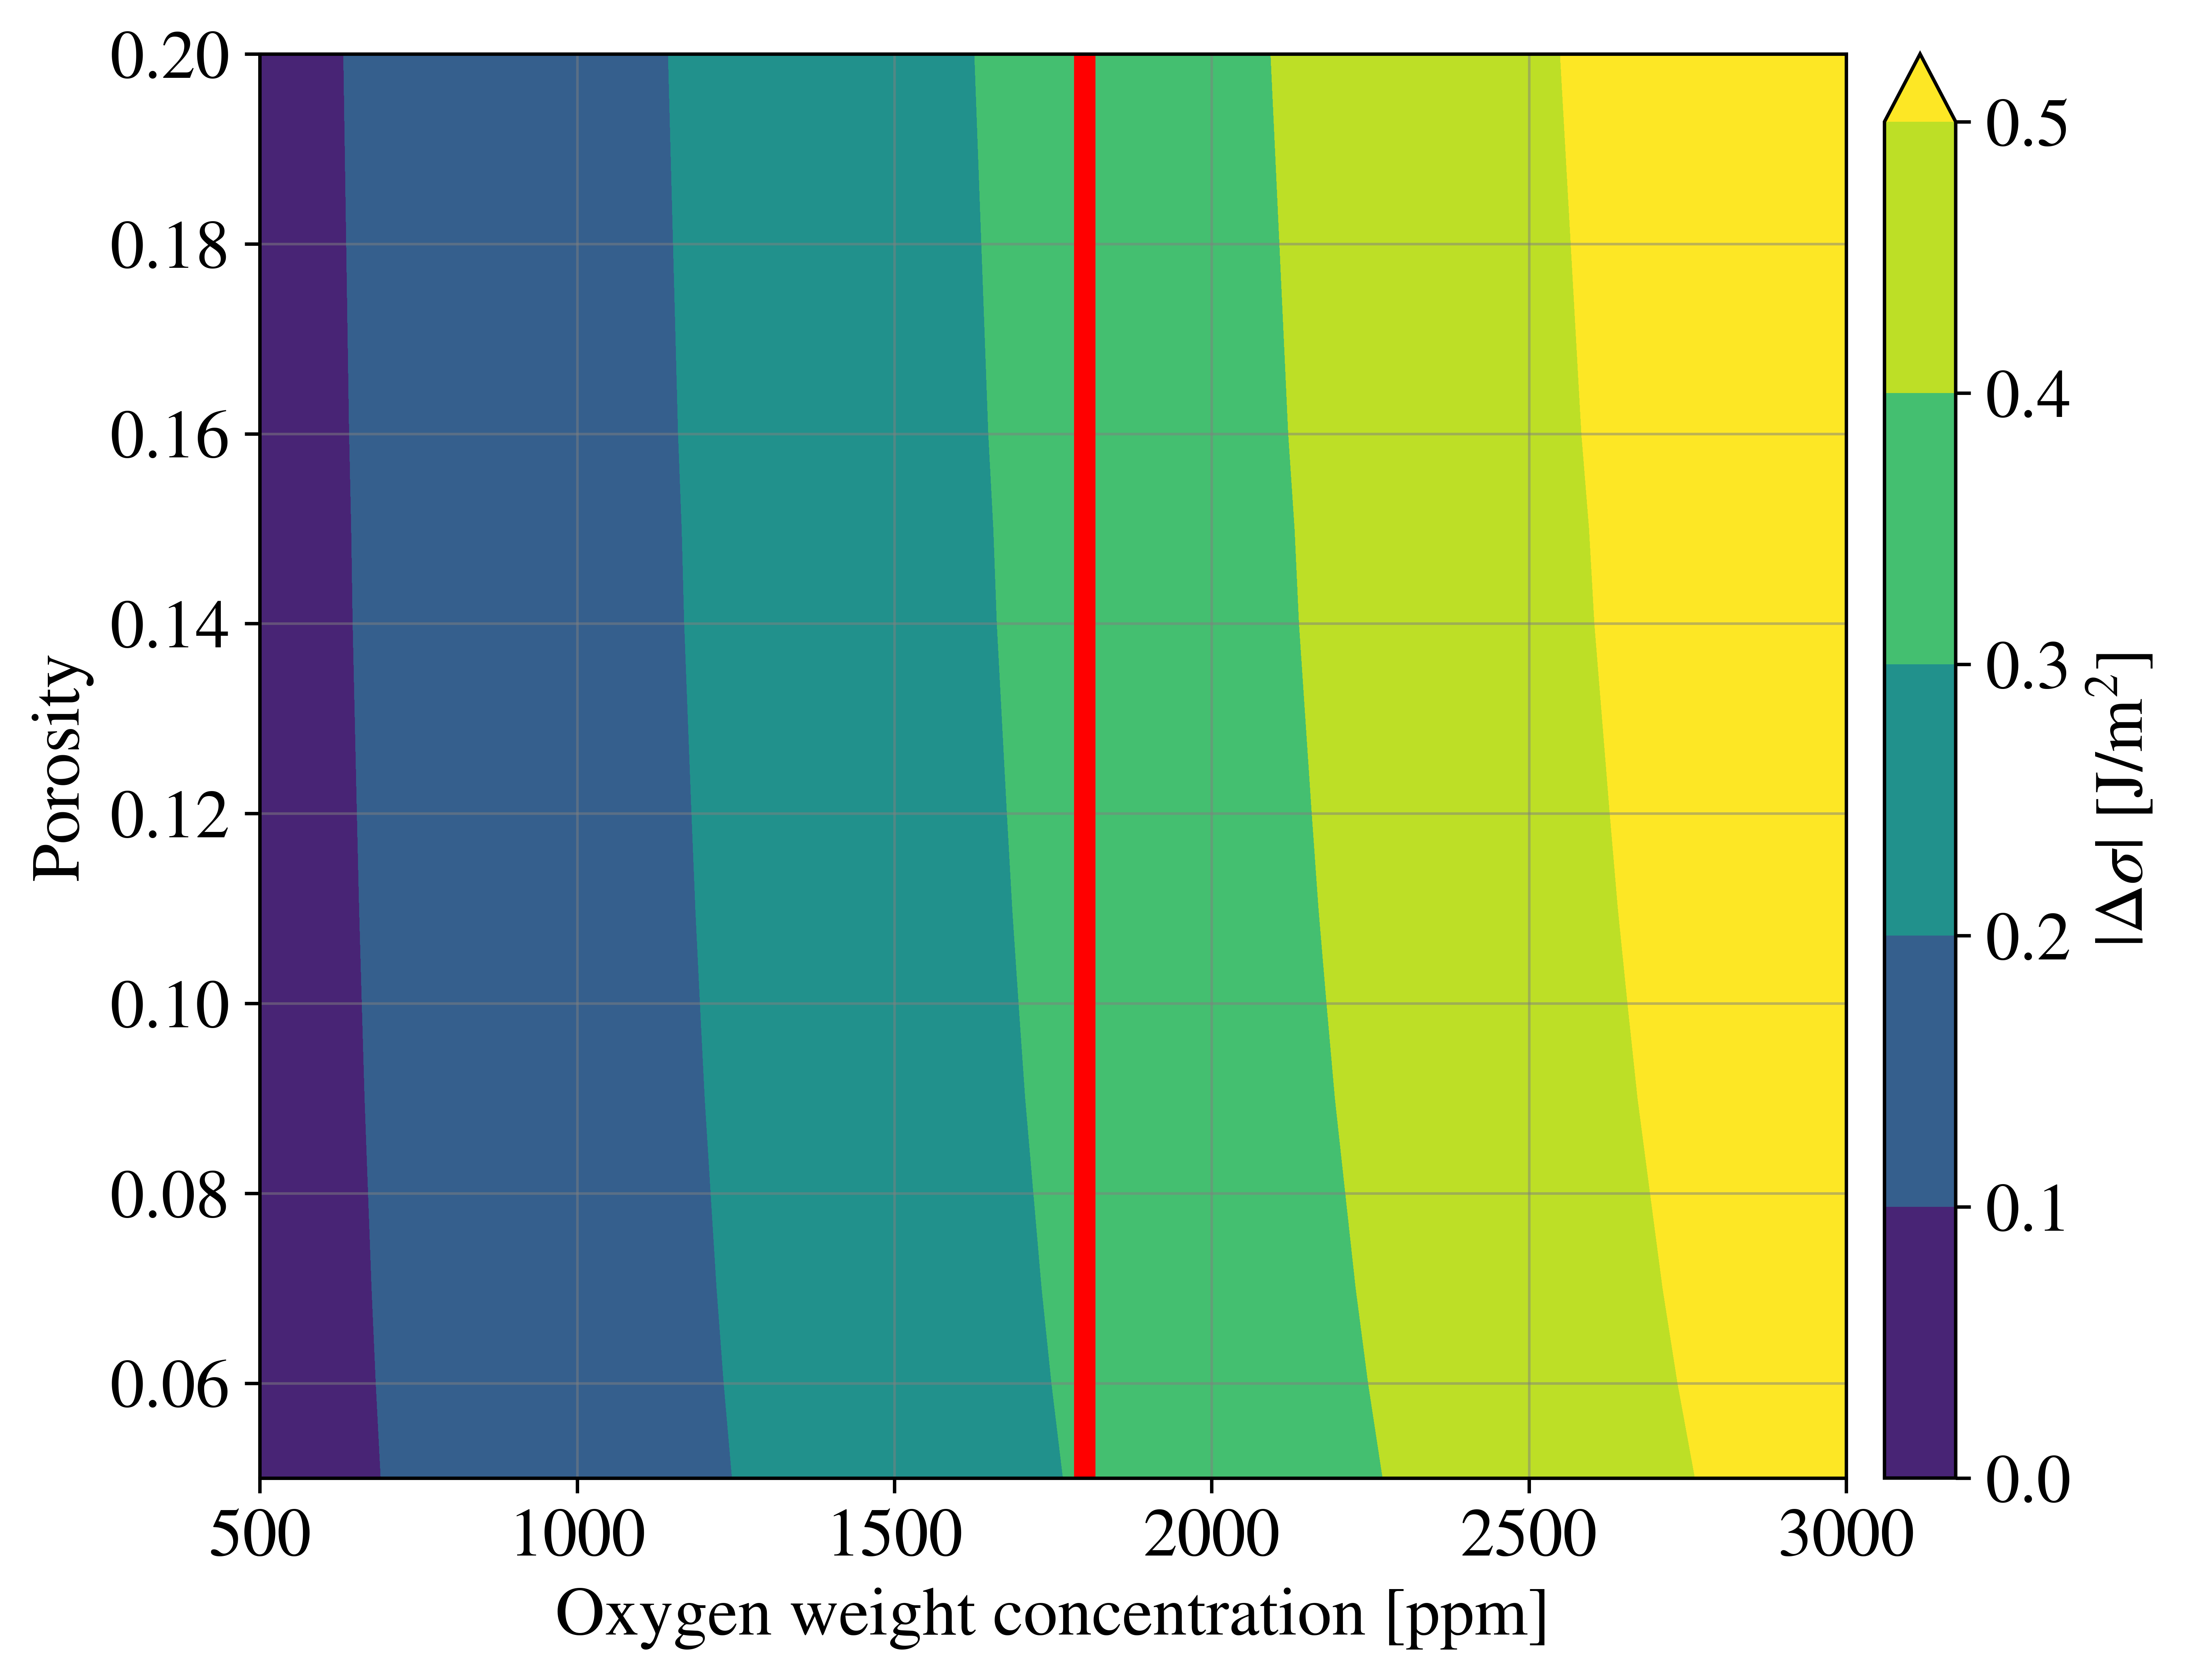
\includegraphics[width=0.5\textwidth]{p_w_abs_gradual_plot_2_5e-08.png}
    \caption{(Color online) Maximum surface energy reduction, $|\Delta \sigma|$ as a function of porosity and oxygen concentration under intermediate stoichiometry for a fixed bubble radius $R_v$ = 25 nm, typical of dislocation and grain-boundary bubbles. The red line marks $w_\text{O}$ = 1800 ppm, the oxygen concentration in UN samples from Ronchi \textit{et al.} \cite{Ronchi1975,Ronchi1978}, used by Rizk \textit{et al.} \cite{Rizk2025} to validate their swelling model. Because $R_v$ is constant, all maxima in $|\Delta \sigma|$ occur at the same temperature.}
    \label{Fig:p_w_plot}
\end{figure}

% \begin{figure}[h!]
% \centering
% \begin{subfigure}{0.48\textwidth}
%     \includegraphics[width=\textwidth]{p_w_abs_gradual_plot.png}
%     \caption{$R_v$ = 50 nm}
%     \label{Fig:p_w_plot}
% \end{subfigure}
% \hfill
% \begin{subfigure}{0.48\textwidth}
%     \includegraphics[width=\textwidth]{R_p_abs_gradual_plot.png}
%     \caption{$w_\text{O}$ = 1800 ppm}
%     \label{Fig:R_p_plot}
% \end{subfigure}
% \hfill
% \begin{subfigure}{0.48\textwidth}
%     \includegraphics[width=\textwidth]{R_w_abs_gradual_plot.png}
%     \caption{$p$ = 15\%}
%     \label{Fig:R_w_plot}
% \end{subfigure}
% \caption{(Color online) Magnitude of the surface energy reduction $|\Delta \sigma|$ (J/m$^2$) as a function of microstructural parameters under intermediate stoichiometry conditions: \textbf{(a)} oxygen concentration and porosity at $R_v$ = 1 nm, \textbf{(b)} void radius and porosity at $w_\text{O}$ = 2500 ppm, and \textbf{(c)} oxygen concentration and void radius at $p$ = 15\%. Red hatched rectangles correspond to the reported ranges of $p$, $w_O$, and $R_v$ in the swelling studies by Ronchi \textit{et al.} \cite{Ronchi1975,Ronchi1978}. The reduction is most pronounced for small cavity radii and high oxygen concentrations, with only weak dependence on porosity.}
% \label{Fig:XXX}
% \end{figure}

\begin{comment}
In UN samples with an oxygen content of 1600 ppm and carbon content of 300 ppm, Mishchenko \textit{et al.} \cite{Mishchenko2021} found 1.5 wt.\% UO$_2$. Thus, increasing the oxygen content to 3500 ppm will most likely lead to the separation of a UO$_2$ phase, unless there is some process by which this oxygen is forced to be in solution.

There are many solubility limits of oxygen in UN reported in the literature: 4400 ppm ($T$ = 1873 K) \cite{Javed1972}, 3910 ppm ($T$ = 300 K) \cite{Jain1993}, 650 ppm ($T$ not reported) \cite{Konovalov2016}, and 6640 ppm ($T$ not reported) \cite{Jaques2015}. In a compilation of experimental studies on oxygen solubility limits in UN, Lyubimov \textit{et al.}  \cite{Lyubimov2014} found that the oxygen solubility in UN is 1930 ppm at a temperature of 1823 K, increases to a peak value of 6640 ppm at 1973 K, and then decreases to about 1540 ppm at 2173 K \cite{Lyubimov2014}. The observed reduction in solubility at temperatures above 2000 K has been attributed to a reduction in carbon content resulting from enhanced CO evaporation at elevated temperatures. This reduction in carbon concentration is hypothesized to lower the oxygen solubility limit, leading to the formation of a separate UO$_2$ phase \cite{Lyubimov2014}. Jain and Ganguly \cite{Jain1993} experimentally observed that the oxygen solubility in UN increases with an increase in UC content. Lyubimov \textit{et al.} \cite{Lyubimov2014} conducted a thermodynamic modeling calculation to quantify this effect and found that a carbon concentration of 720 ppm increases the oxygen solubility by a factor of 4--5. Based on this analysis, we can see that a carbon content of 720 ppm is large enough to keep an oxygen concentration of 3500 ppm in solution and suppress UO$_2$ phase separation, thus enhancing void swelling in UN.
\end{comment}

In UN samples with an oxygen content of 1600 ppm and carbon content of 300 ppm, Mishchenko \textit{et al.} \cite{Mishchenko2021} found 1.5 wt.\% UO$_2$. Thus, having an oxygen content of, e.g., 1800 ppm will most likely lead to the separation of a UO$_2$ phase, unless there is some process by which this oxygen is forced to be in solution. There are many solubility limits of oxygen in UN reported in the literature, ranging from 650 ppm to 6640 ppm \cite{Javed1972,Jain1993,Konovalov2016,Jaques2015}. Lyubimov \textit{et al.} \cite{Lyubimov2014} conducted a thermodynamic modeling calculation and found that a carbon concentration of 720 ppm increases the oxygen solubility by a factor of 4--5. Based on this analysis, a carbon content of 720 ppm is large enough to keep an oxygen concentration of 3000 ppm in solution and suppress UO$_2$ phase separation, thus leading to $|\Delta \sigma| > 0.5$ J/m$^2$ (see \cref{Fig:p_w_plot}) and enhanced void swelling in UN.

\section{Discussion}

This study presents a novel model that integrates first-principles calculations with defect chemistry to quantify the role of oxygen impurities in stabilizing voids and fission gas bubbles in UN. To our knowledge, this is the first model to establish a quantitative link between oxygen concentration and void nucleation thermodynamics in UN. By capturing how oxygen segregates to void surfaces and reduces the surface energy, this work advances the mechanistic understanding of swelling phenomena in oxygen-contaminated nuclear fuels. Importantly, this surface energy reduction is found to be most pronounced for void embryos ($R_v$ = 1 nm) at intermediate temperatures (1300--1700~K), aligning with the temperature range associated with the onset of breakaway swelling in UN \cite{Ronchi1975,Ronchi1978,Rizk2025}. Noting that the range of operating temperatures in liquid metal-cooled fast reactors is 800--2000 K \cite{Turos1990}, these findings highlight oxygen adsorption as a critical factor in facilitating void nucleation under conditions typical of reactor environments.

The model provides predictive capabilities by mapping the dependence of surface energy reduction on key physical parameters, including temperature, porosity, void radius, and oxygen concentration. Parametric analysis reveals that surface energy reduction is strongly influenced by oxygen concentration and void radius, while being nearly independent of porosity. In particular, small bulk voids and bubbles experience a significant stabilization effect from oxygen at intermediate temperatures, highlighting the role of oxygen in the early stages of void or fission gas bubble formation. These insights may provide a physically grounded explanation for the association between oxygen content and accelerated swelling observed in experimental studies of mixed uranium carbide/nitride fuels~\cite{Rogozkin2003}. Furthermore, the generality of the approach allows for its extension to other materials systems and integration into mesoscale models and fuel performance codes, offering a path toward multiscale modeling of chemically assisted swelling in nuclear materials.

Rizk \textit{et al.} adopted a surface energy of 1.11 J/m$^2$, computed using the empirical potential developed by Kocevski \textit{et al.} \cite{Kocevski2022II}. In contrast, our DFT calculations yield a higher value of 1.59 J/m$^2$ for a planar surface. This 0.48 J/m$^2$ discrepancy, neglecting curvature corrections, likely stems from the known tendency of the Kocevski potential to underestimate defect energetics in UN~\cite{AbdulHameed2024}, a limitation that appears to manifest here as well. Substituting $\sigma$ = 1.59 J/m$^2$ into the model of Rizk \textit{et al.} would suppress both fission gas swelling and release, necessitating recalibration of other model parameters to preserve agreement with experiment. This discrepancy highlights the need for a mechanism that lowers surface energy in irradiated UN. We propose that oxygen adsorption at bubble surfaces fulfills this role, enabling the levels of swelling and gas release observed experimentally. A reduction in surface energy thus appears essential to reconcile the mechanistic model with experimental data. Notably, the oxygen concentration reported by Ronchi \textit{et al.} ($w_\text{O}$ = 1800 ppm) corresponds to a predicted surface energy reduction of 0.3--0.4 J/m$^2$, closely matching the gap between our DFT value and that used by Rizk \textit{et al.}

% An elevated surface energy would have significant consequences for the thermodynamic and kinetic evolution of fission gas bubbles in the mechanistic model. The equilibrium internal pressure of a bubble, given by the modified Young–Laplace relation $P_{\text{eq}} = 2\sigma / R_v - s_h$, scales linearly with $\sigma$. Thus, increasing the surface energy raises the equilibrium pressure required for mechanical stability at a given radius, resulting in more severe over-pressurization for the same gas content. This, in turn, enhances the driving force for vacancy absorption while simultaneously increasing the energetic penalty associated with surface formation. The net effect is a suppression of bubble nucleation and growth, particularly for dislocation-mediated intragranular bubbles that dominate swelling near the breakaway temperature. Moreover, grain boundary bubbles, which are already over-pressurized in the model, would experience even greater resistance to expansion, thereby delaying interconnection and fission gas release. These effects would collectively shift the Vitanza-type release threshold to higher temperatures and burnups, leading to unrealistically low gas release predictions and artificial retention of gas within the fuel matrix. 

Despite its contributions, the present model includes several simplifications that merit further investigation. First, the surface adsorption energy of oxygen is assumed to be independent of surface coverage, which may not hold at high impurity concentrations where impurity-impurity interactions become significant. Additionally, configurational and vibrational entropy contributions are neglected, which may affect the temperature dependence of defect formation and migration energies, particularly at elevated temperatures. Further, the kinetic parameter used to model oxygen segregation is introduced in an \textit{ad hoc} manner, limiting the model's capability to capture time-dependent or rate-limited processes. Finally, the influence of sinks such as grain boundaries and second-phase precipitates, which may trap oxygen or alter defect transport, is also not incorporated.

A further limitation is that the current model isolates oxygen as the sole impurity species. In reality, fission products and other impurities, such as carbon, krypton, and xenon, may co-segregate or interact with oxygen, altering the energetics and morphology of vacancy clusters. Notably, our calculations indicate that substitutional oxygen on nitrogen sites binds to uranium-site vacancies and noble gas atoms (i.e., Kr$_\text{U}$, Xe$_\text{U}$) with energies around $-0.4$~eV. Whether this binding promotes the stabilization of voids or instead alters gas mobility and clustering behavior is not yet fully understood. Future studies should assess how such interactions affect oxygen-assisted swelling in fission environments.

Finally, while the role of carbon in increasing oxygen solubility and suppressing UO$_2$ precipitation in UN is qualitatively known, the impact of carbon content on void stabilization was not explicitly addressed in this model. Given that carbon can modulate the chemical potential of oxygen and influence its incorporation and redistribution, a natural extension of this work is to explore the combined effects of carbon and oxygen on defect energetics and swelling behavior in UN. The framework developed here is directly applicable to this scenario.

\section{Conclusions}

This work develops a first-principles-based thermodynamic framework that quantifies how oxygen impurities interact with void surfaces in UN, leading to a reduction in the surface energy, $|\Delta \sigma|$. The model incorporates DFT-derived energetics, oxygen diffusivity, defect chemistry, and microstructural parameters to assess the extent of surface stabilization.

Key findings can be summarized as follows. Substitutional oxygen on nitrogen surface sites ($\text{O}_\text{N}^\text{(s)}$) is the dominant contributor to surface energy reduction. Oxygen in surface hollow sites ($\text{O}_i^\text{(s)}$) has a minor, and occasionally adverse, effect on $|\Delta \sigma|$. The dependence of $|\Delta \sigma|$ on key parameters is summarized below:
\begin{itemize}
    \item \textit{Oxygen concentration ($w_\text{O}$):} The surface energy reduction scales linearly with oxygen content.
    \item \textit{Void radius ($R_v$):} $|\Delta \sigma|$ is most pronounced for small voids. Larger voids require higher temperatures to reach meaningful oxygen coverage and experience a slightly smaller $|\Delta \sigma|$.
    \item \textit{Porosity ($p$):} The surface energy reduction is found to be largely insensitive to porosity.
    \end{itemize}

\vspace{0.5cm}

For small voids and bubbles ($R_v$ = 1--10 nm), $|\Delta \sigma|$ exhibits three regimes in its dependence on temperature:
    \begin{itemize}
    \item \textit{Low temperatures:} $|\Delta \sigma| \approx 0$ due to limited oxygen diffusivity.
    \item \textit{Intermediate temperatures:} $|\Delta \sigma|$ reaches its maximum as the competing effects of oxygen solubility and diffusion kinetics are optimally balanced. This regime coincides with the onset of breakaway swelling in UN.
    \item \textit{High temperatures:} $|\Delta \sigma|$ decreases due to enhanced bulk solubility, which disfavors surface segregation.
    \end{itemize}

The reduction in surface energy can be approximately expressed as:
\[
|\Delta \sigma| \approx \eta \, n_\text{O} \, \alpha_1 \, |E_\text{seg}^\text{eff}|,
\]
where $\eta$ is a geometric factor that depends on $p$ and $R_v$, $n_\text{O}$ is the oxygen number density, $\alpha_1$ is a kinetic correction factor, and $E_\text{seg}^\text{eff}$ is the effective segregation energy. The reduction in $\sigma$ lowers the thermodynamic barrier for void and bubble formation. For the reference case of $w_\text{O}$ = 1800 ppm in UN \cite{Ronchi1975}, our model predicts a surface energy reduction of about 0.3--0.4 J/m$^2$ for dislocation and grain-boundary bubbles. This aligns closely with the discrepancy between our DFT-calculated surface energy (1.59 J/m$^2$) and the value adopted by Rizk \textit{et al.} \cite{Rizk2025} in their swelling model (1.11 J/m$^2$). The oxygen-induced reduction in $\sigma$ thus can offer a mechanistic explanation for the experimentally observed levels of swelling and fission gas release in UN. % Weak binding between $\text{O}_\text{N}^\text{(b)}$ and uranium vacancies ($v_\text{U}$) or noble gas atoms ($\text{Kr}_\text{U}$ and $\text{Xe}_\text{U}$) may contribute to the stabilization of void embryos.

Overall, this work provides a physically rigorous model for incorporating oxygen effects into mechanistic swelling models of UN. The framework is extendable to other chemical impurities such as carbon and can be integrated into mesoscale and fuel performance models to predict chemically-assisted bubble swelling in nuclear fuels.

\section{Acknowledgments}

This work was supported by the DOE-NE and Westinghouse Electric Company under contract DE-NE0008824. This research used resources provided by the Los Alamos National Laboratory Institutional Computing Program, which is supported by the U.S. Department of Energy National Nuclear Security Administration under Contract No. 89233218CNA000001. Los Alamos National Laboratory, an affirmative action/equal opportunity employer, is operated by Triad National Security, LLC, for the National Nuclear Security Administration of the U.S. Department of Energy under Contract No. 89233218CNA000001. This research also made use of the resources of the High-Performance Computing Center at Idaho National Laboratory, which is supported by the Office of Nuclear Energy of the U.S. Department of Energy and the Nuclear Science User Facilities under Contract No. DE-AC07-05ID14517. Mohamed AbdulHameed thanks William Neilson, Conor Galvin, and Kai Duemmler for the great help provided while conducting this research.

\appendix

\section{Derivation of the formulas for $[ \text{N}_\text{N}^\text{(s)} ]$ and $[ v_i^\text{(s)} ]$}
\label{App1}

The area associated with an N atom on the surface is $a^2/2$, where $a$ is the lattice constant. The total surface area of the internal voids is $N_v \times 4 \pi R_v^2$, where $N_v$ is the total number of voids, calculated as:
\begin{equation}
N_v = \frac{ p V_0 }{ \frac{4}{3} \pi R_v^3 },
\end{equation}
where $V_0$ is the total system volume. Then, the number of $\text{N}_\text{N}^\text{(s)}$ sites is:
\begin{equation}
\text{Number of } \text{N}_\text{N}^\text{(s)} = \frac{ N_v \times 4 \pi R_v^2 } { a^2 / 2 }. 
\label{Eq:1}
\end{equation}
To get the site fraction of $\text{N}_\text{N}^\text{(s)}$, we need to divide its total number by the number of formula units. The number of formula units is:
\begin{equation}
\text{Number of formula units} = \frac{V_0 (1 - p)}{ a^3 / 4 }, 
\label{Eq:2}
\end{equation}
where $V_0 (1 - p)$ is the occupied volume, and $a^3 / 4$ is the volume of a single formula unit. Dividing \cref{Eq:1} by \cref{Eq:2}, we arrive at:
\begin{equation}
[ \text{N}_\text{N}^\text{(s)} ] = \frac{p V_0}{ \frac{4}{3} \pi R_v^3 } \frac{4 \pi R_v^2}{a^2/2}  \frac{ a^3/4 }{ V_0 (1 - p) } = \frac{3}{2} \frac{p}{1-p} \frac{a}{R_v}.
\label{Eq:NNs}
\end{equation}

The same steps can be followed to get an expression for $[v_i^\text{(s)}]$, provided that we pay attention to the following differences: First, the area occupied by a vacant site on the surface is $a^2/4$. Then, the number of $v_i^\text{(s)}$ sites is:
\begin{equation}
\text{Number of } v_i^\text{(s)} = \frac{ N_v \times 4 \pi R_v^2 } { a^2 / 4 }.
\end{equation}
To get the site fraction of $v_i^\text{(s)}$, we need to divide its total number by the number of formula units in the occupied volume (i.e., \cref{Eq:2}), and then divide by 2 because there are 2 tetrahedral interstitial sites per formula unit, either in the bulk material or on the surface. In the case of $[ \text{N}_\text{N}^\text{(s)} ]$, there was one N atom (or site) per formula unit. Then, the site fraction of $v_i^\text{(s)}$ is: 
\begin{equation}
[ v_i^\text{(s)} ] = \frac{1}{2} \frac{p V_0}{ \frac{4}{3} \pi R_v^3 } \frac{4 \pi R_v^2}{ a^2/4}  \frac{ a^3/4 }{ V_0 (1 - p) } = \frac{3}{2} \frac{p}{1-p} \frac{a}{R_v},
\label{Eq:Vis}
\end{equation}
which is the same expression for $[ \text{N}_\text{N}^\text{(s)} ]$. Note that both \cref{Eq:NNs,Eq:Vis} are independent of $V_0$. As outlined in \cref{Sec:DefE}, the adsorption energy of O atoms in above-U sites is the same as that of O in a hollow site (\cref{Tab:Ead}). To account for this in our model, the available adsorption sites are doubled by multiplying $[ v_i^\text{(s)} ]$ by 2. In this way, the analysis is simplified by only considering $\text{O}_i^{\text{(s)}}$. The final expression reads:
\begin{equation}
[v_i^{\text{(s)}}] = \frac{3p}{1-p} \frac{a}{R_v}.
\end{equation}

\section{Derivation of the formula for surface energy change as a function of adsorbate atom concentration}
\label{App2}

Suppose we have an impurity atom that got adsorbed on a pristine surface. The surface energy after absorption is: 
\begin{equation}
\sigma = \sigma_0 + \Delta \sigma,
\end{equation}
where $\sigma_0$ is the energy of the pristine surface before adsorption, and $\Delta \sigma$ is the surface energy change due to impurity adsorption. The change in the surface energy can be expressed as:
\begin{equation}
\Delta \sigma = \sigma_\text{surf+ad} - \sigma_\text{surf},
\end{equation}
where:
\begin{equation}
\sigma_\text{surf} = \frac{1}{A} \left[ E_\text{surf} - N_\text{U} \mu_\text{U} - N_\text{N} \mu_\text{N} \right],
\end{equation}
and:
\begin{equation}
\sigma_\text{surf+ad} = \frac{1}{A} \left[ E_\text{surf+ad} - N_\text{U} \mu_\text{U} - N_\text{N} \mu_\text{N} - N_\text{ad} \mu_\text{ad} \right].
\end{equation}
Then,
\begin{equation}
\Delta \sigma = \frac{1}{A} \left[ E_\text{surf+ad} - E_\text{surf} - N_\text{ad} \mu_\text{ad} \right].
\end{equation}

From the definition of the adsorption energy, i.e., \cref{Eq:Ead}, the change in the surface energy is:
\begin{equation}
\Delta \sigma = \frac{1}{A} \left[ N_\text{ad} ( E_\text{ad} + \mu_\text{ad} ) - N_\text{ad} \mu_\text{ad} \right] = \frac{1}{A} N_\text{ad} E_\text{ad}. 
\end{equation}

If we have a specific concentration of an impurity that can get adsorbed on different sites on the surface, with each site type having its own adsorption energy, then:
\begin{equation}
\Delta \sigma = \frac{1}{A} \left[ \sum_i N_\text{ad}^i E_\text{ad}^i \right].
\end{equation}

The same line of thought can be used to derive an expression for the surface energy change upon introducing vacancies to a previously pristine surface. For the general case where we introduce both adsorbate atoms and vacancies to a surface, the total surface energy change is:
\begin{equation}
\Delta \sigma = \frac{1}{A} \left[ \sum_i N_\text{ad}^i E_\text{ad}^i + \sum_j N_d^j E_f^j \right].
\label{Eq:DeltaSigma}
\end{equation}

This can be related to the relative concentrations calculated earlier by noticing that:
\begin{equation}
N_\text{ad}^i = N_\text{O} \frac{N_\text{ad}^i}{N_\text{O}} \approx N_\text{O} \frac { [ \text{O}_\text{X}^{\text{(s)}} ] } { [ \text{O}_\text{N}^{\text{(b)}} ] },   
\label{Eq:Nad}
\end{equation}
where $N_\text{O}$ is the total number of oxygen atoms in the sample and X $\in$ \{N, $i$\}. Finally, we can relate $N_d$, i.e., the total number of surface defects, to the concentrations calculated earlier by a similar argument. Assuming the surface defect is $v_\text{N}^{\text{(s)}}$, we have:
\begin{equation}
N_d = [ v_\text{N}^{\text{(s)}} ] \times \text{Number of N$_\text{N}^\text{(s)}$} = [ v_\text{N}^{\text{(s)}} ] \frac{A_v}{a^2 / 2}, 
\label{Eq:Nd}
\end{equation}
where we have made use of \cref{Eq:1} with $A_v$ being the total area of the void surface.

The total number of oxygen atoms in the system is not a useful parameter. Instead, we need the formulas to be expressed in terms of some measure of oxygen concentration. The number of voids is expressed in terms of both the void surface area and the void volume as:
\begin{equation}
N_v = \frac{A_v}{4 \pi R_v^2} = \frac{ p V_0 }{ \frac{4}{3} \pi R_v^3 }.
\label{Eq:Nv}
\end{equation}
From \cref{Eq:Nv}, the total void surface area is:
\begin{equation}
A_v = \frac{3 p V_0}{R_v} = \frac{3}{R_v} \frac{p}{1-p} V.
\label{Eq:Av}
\end{equation}
Then,
\begin{equation}
\frac {N_\text{O}} {A_v} = \frac {R_v} {3} \frac{1-p} {p} \frac {N_\text{O}} {V} = \frac {R_v} {3} \frac{1-p} {p} \frac {N_\text{O}} { 2 N_\text{UN} \cdot a^3/8 } \approx \frac{8}{3} \frac{1-p}{p} \frac{R_v}{a^3} c_\text{O}, 
\label{Eq:NOAv}
\end{equation}
where $N_\text{UN}$ is the number of formula units in the occupied volume, $a^3/8$ is the average volume per atom of UN, and $c_\text{O}$ is the atomic fraction of O atoms which is approximately $c_\text{O} \approx N_\text{O}/( 2N_\text{UN})$. The oxygen impurity concentration in UN is usually expressed as parts per million (ppm) or weight fractions. The relation between atomic fraction, $c_\text{O}$, and weight fraction, $w_\text{O}$, is:
\begin{equation}
c_\text{O} = \frac { M_\text{UN} w_\text{O} } { M_\text{UN} w_\text{O} + 2 M_\text{O} ( 1 - w_\text{O} ) },
\label{Eq:cO}
\end{equation}
where $M_\text{UN}$ and $M_\text{O}$ are the molar weights of UN and O, respectively. From \cref{Eq:cO}, $w_\text{O}$ can be expressed in terms of $c_\text{O}$ as:
\begin{equation}
w_\text{O} = \frac{ 2 M_\text{O} c_\text{O} }{ 2 M_\text{O} c_\text{O} + M_\text{UN} ( 1 - c_\text{O} ) }.
\end{equation}
Substituting \cref{Eq:Nad,Eq:NOAv,Eq:Nd} into \cref{Eq:DeltaSigma}, the change in surface energy becomes:
\begin{equation}
\Delta \sigma = \frac{8}{3} \frac{1-p}{p} \frac{R_v}{a^3} c_\text{O} \left[ \frac{ [ \text{O}_\text{N}^{\text{(s)}} ] }{ [ \text{O}_\text{N}^{\text{(b)}} ] }  E_\text{ad}( \text{O}_\text{N}^{\text{(s)}} ) + \frac{ [ \text{O}_i^{\text{(s)}} ] }{ [ \text{O}_\text{N}^{\text{(b)}} ] }  E_\text{ad}( \text{O}_i^{\text{(s)}} ) \right] + \frac{2}{a^2} [ v_\text{N}^{\text{(s)}} ] E_f ( v_\text{N}^{\text{(s)}} ).
\end{equation}

To take kinetics into account, the concentrations of the different oxygen surface defects must be corrected for the low oxygen diffusivity at low temperatures. Note that the increased oxygen solubility is inherently incorporated in the thermodynamic model. According to Zinkle and Lee \cite{Zinkle1990}, as a first approximation, the concentrations of oxygen surface defects can be multiplied by a parameter $\alpha$ that we term the kinetic correction, and that depends on the diffusivity of different oxygen defect types. Thus, the final expression for the change in surface energy becomes:
\begin{equation}
\Delta \sigma = \frac{8}{3} \frac{1-p}{p} \frac{R_v}{a^3} c_\text{O} \left[ \alpha_1 \frac{ [ \text{O}_\text{N}^{\text{(s)}} ] }{ [ \text{O}_\text{N}^{\text{(b)}} ] }  E_\text{ad}( \text{O}_\text{N}^{\text{(s)}} ) + \alpha_2 \frac{ [ \text{O}_i^{\text{(s)}} ] }{ [ \text{O}_\text{N}^{\text{(b)}} ] }  E_\text{ad}( \text{O}_i^{\text{(s)}} ) \right] + \frac{2}{a^2} [ v_\text{N}^{\text{(s)}} ] E_f ( v_\text{N}^{\text{(s)}} ),
\end{equation}
where $\alpha_1$ and $\alpha_2$ are the kinetic corrections for the defects $\text{O}_\text{N}^\text{(s)}$ and $\text{O}_i^{\text{(s)}}$, respectively. Conceptually, $\alpha_i$ stems from the fraction of diffusing oxygen atoms that encounter a void embryo during the void nucleation time, and, thus, can be defined as \cite{Zinkle1990}:
\begin{equation}
\alpha_i =
\begin{cases}
    \sqrt{D_i t}/\lambda_v & \text{if } \sqrt{D_i t}/\lambda_v < 1, \\
    1 & \text{if } \sqrt{D_i t}/\lambda_v \geq 1,
\end{cases}    
\end{equation}
where $D_i$ is the diffusivity of the relevant defect, $t$ is the void nucleation time, and $\lambda_v$ is the mean free path between voids, defined as $\lambda_v = n_v^{-1/3}$ \cite{Olander2021}, where $n_v = p / ( \frac{4}{3} \pi R_v^3 ) $ is the void number density.

\FloatBarrier

\section{Supplementary information}
\label{App3}

% \printnomenclature

\begin{figure}[h!]
\centering
\begin{subfigure}{0.45\textwidth}
    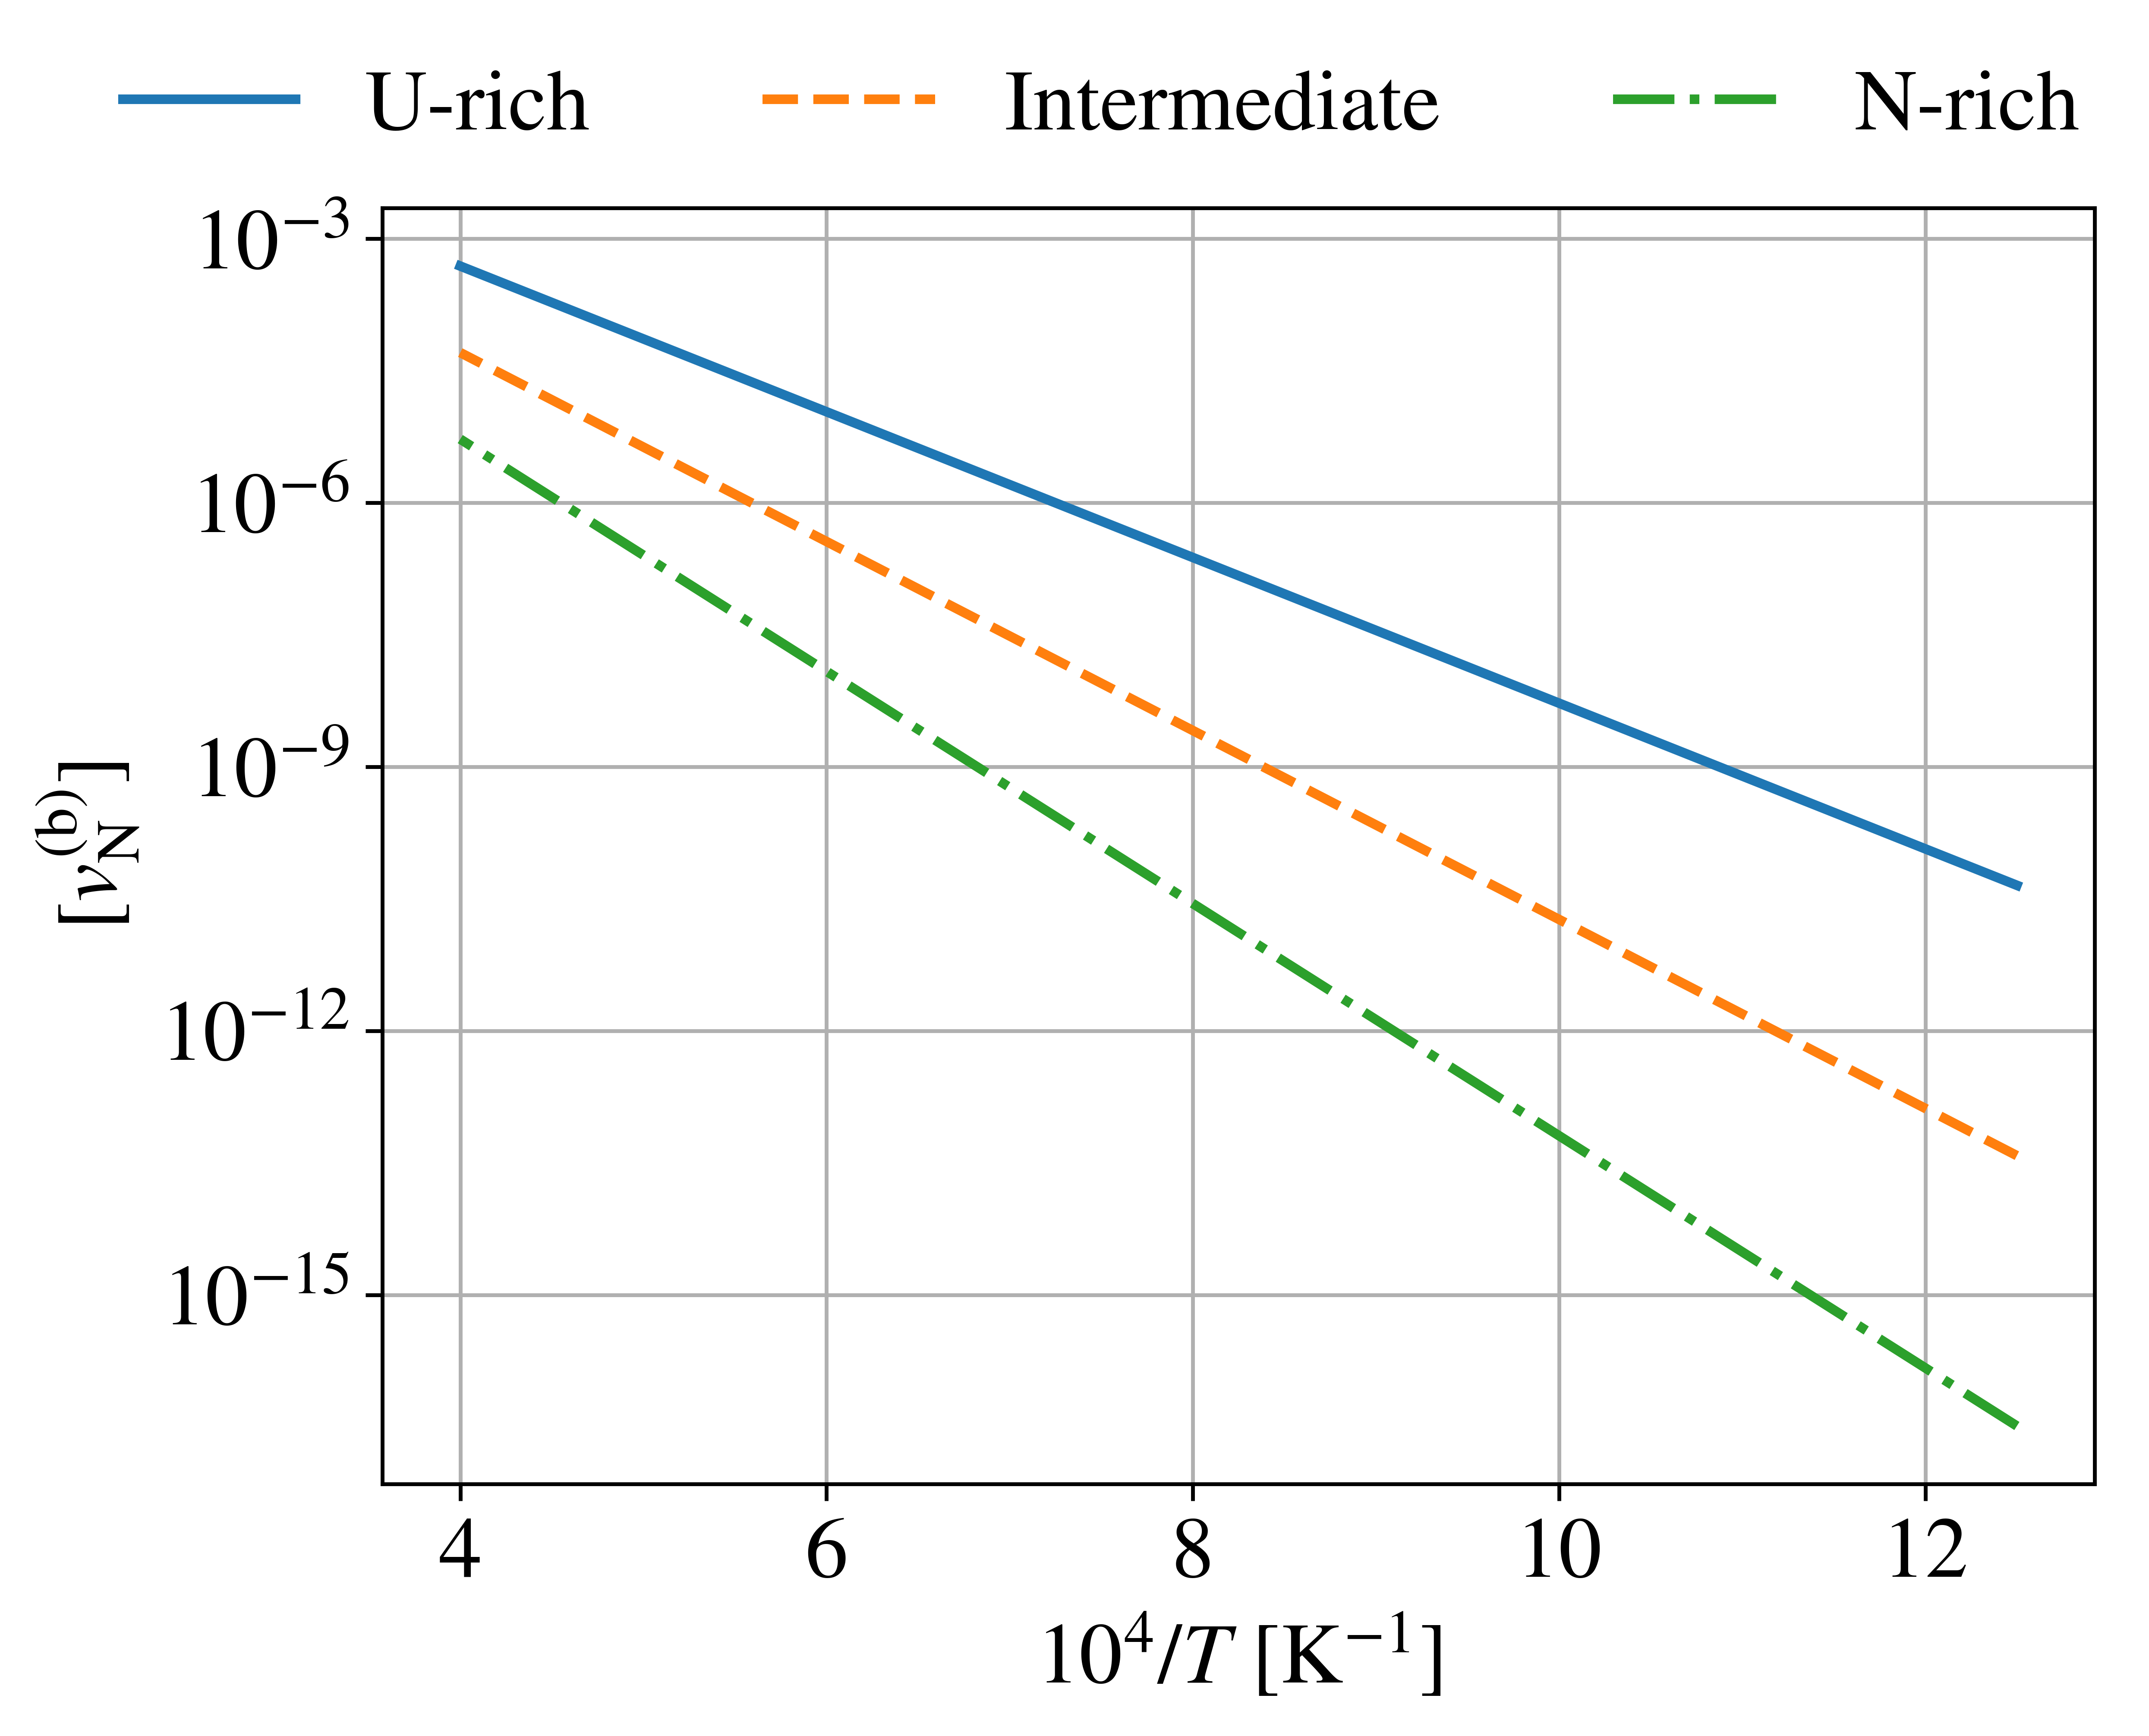
\includegraphics[width=\textwidth]{VN.png}
    \caption{}
    \label{Fig:VN}
\end{subfigure}
\hfill
\begin{subfigure}{0.45\textwidth}
    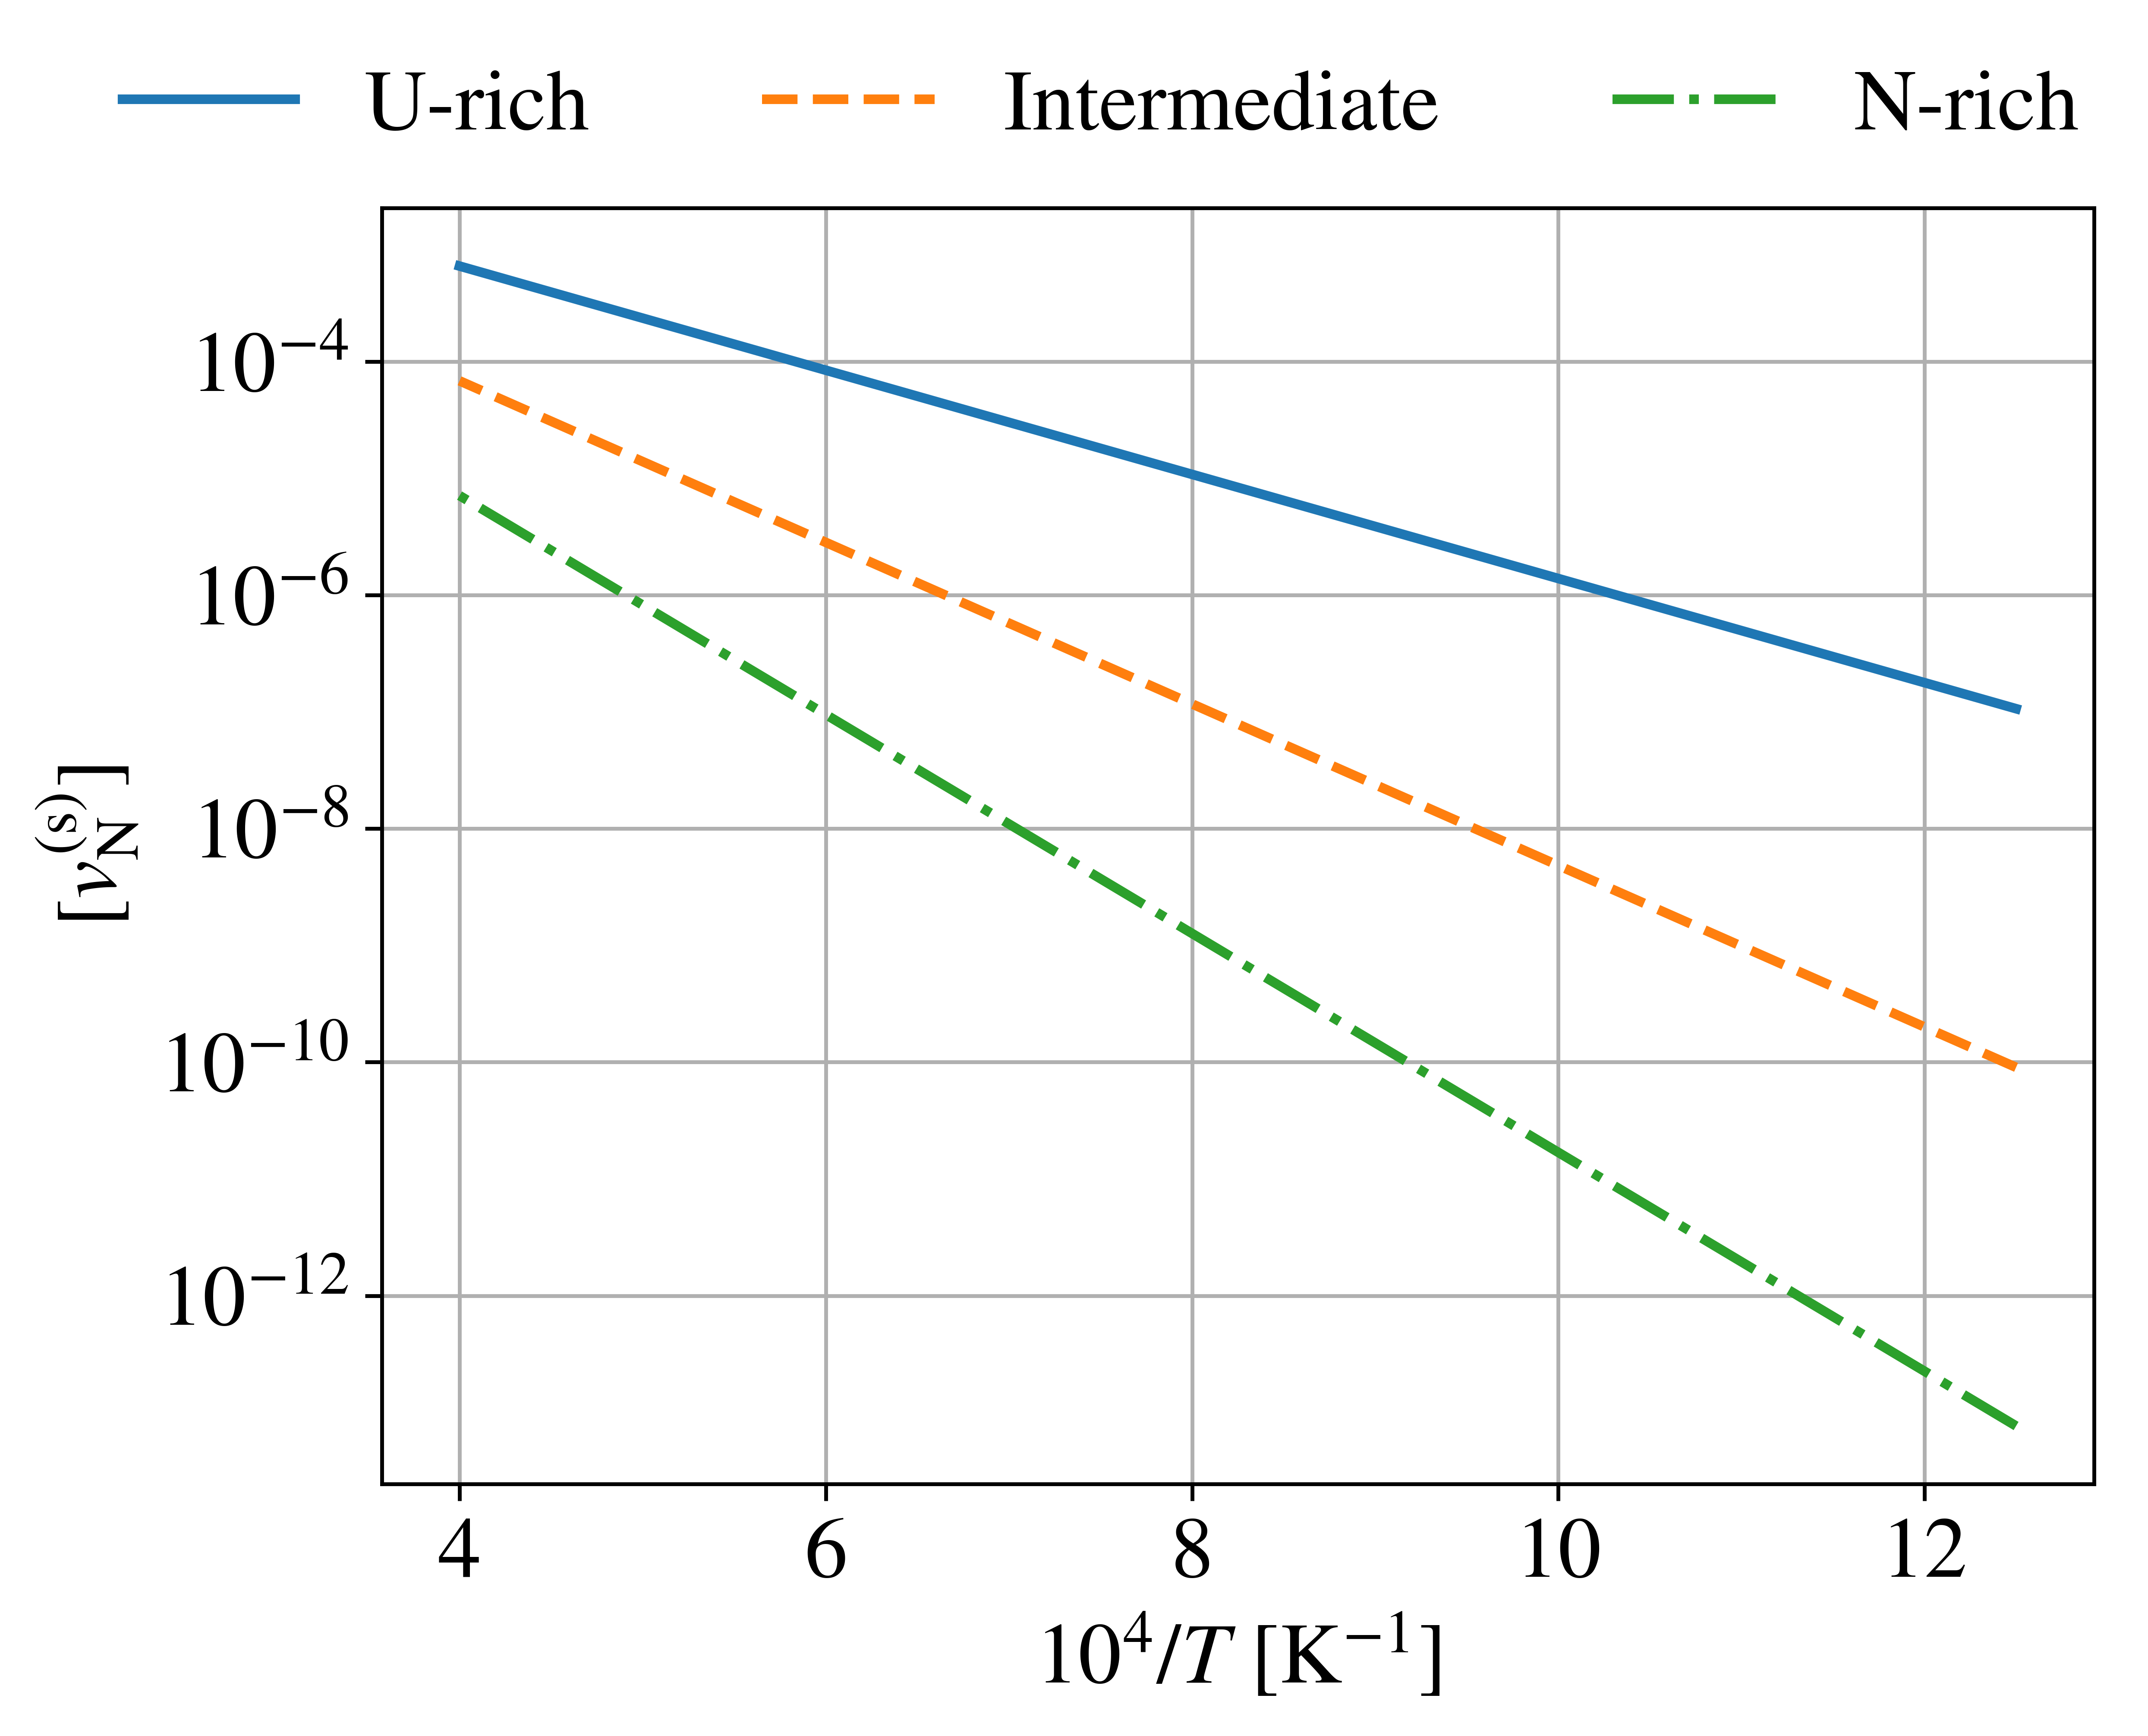
\includegraphics[width=\textwidth]{VNs.png}
    \caption{}
    \label{Fig:VNs}
\end{subfigure}
\caption{\textbf{(a)} Concentration of N vacancies in bulk UN calculated from the formation energies in \cref{Tab:EfVN}. \textbf{(b)} Concentration of N vacancies on the UN (001) surface calculated from the formation energies in \cref{Tab:EfVN}.}
\label{1}
\end{figure}

\begin{figure}[h!]
    \centering
    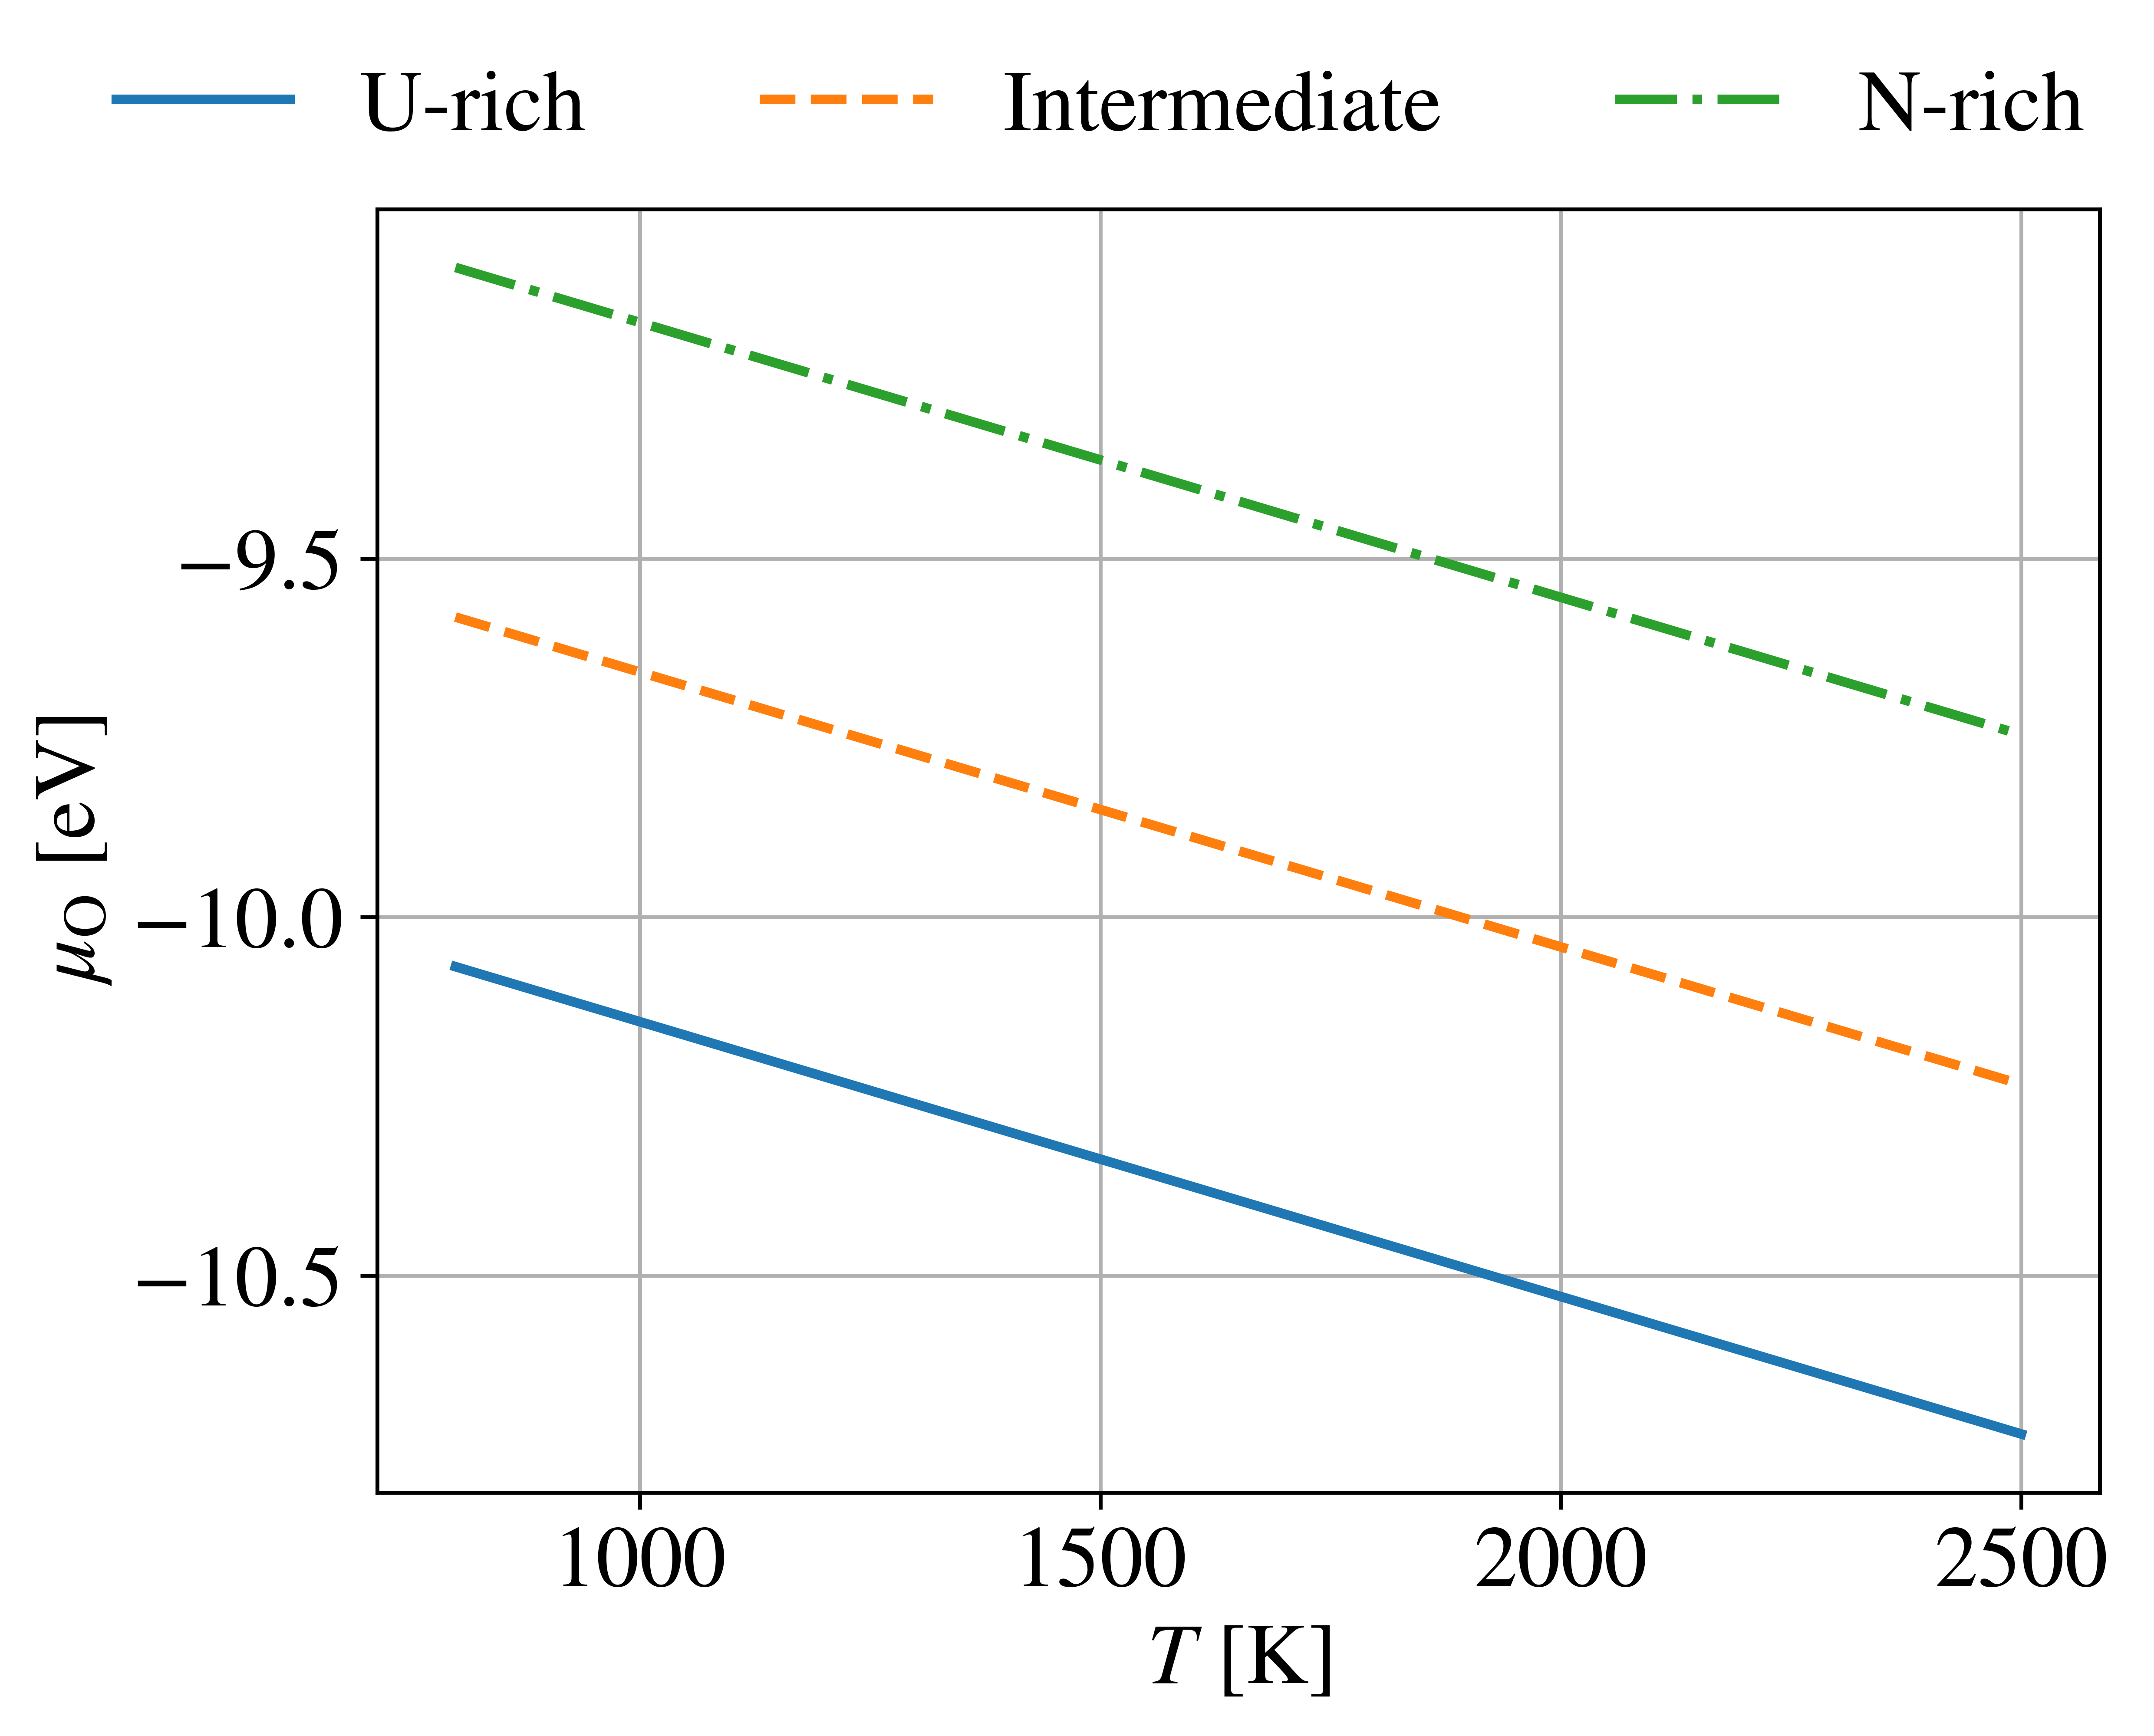
\includegraphics[width=0.45\textwidth]{uO.png}
    \caption{Oxygen chemical potential as calculated based on \cref{Eq:OxygenTruePot}.}
    \label{Fig:uO}
\end{figure}

\FloatBarrier

\bibliographystyle{elsarticle-num}
\bibliography{ref}

\end{document}